
%____________________DOCUMENT PREAMBLE_________________________________
\documentclass[12pt]{report}
\usepackage{appendix}
\usepackage{graphicx}
\usepackage{sidecap}
\usepackage{wrapfig}
\usepackage{float}
\usepackage{supertabular}
\usepackage{array}
\usepackage{threeparttable}
\usepackage{booktabs}
\usepackage[margin=3cm]{geometry}
\usepackage{setspace}
\usepackage{url}
\usepackage{amssymb}
\usepackage{amsmath}
\usepackage[version=3]{mhchem}  %Chemical compounds \ce{(NH4)2SO4}.
%\usepackage{fixltx2e}
\usepackage{indentfirst}
\usepackage{subcaption}
\usepackage{caption}
\usepackage{pdflscape}
\usepackage{lipsum}
\usepackage{blindtext}
%\usepackage[nottoc]{tocbibind} %So bibliography won't appear as a chapter in the document
\usepackage{pgfplots}
\usepackage{fancyhdr}
\usepackage{pgfplotstable}
\usepackage{colortbl}
\usepackage{xcolor}
\usepackage{multirow}
\usepackage{tocloft}
\usepackage{notoccite} % PREVENTS CITES IN CAPTIONS FROM MISNUMBERING YOUR REFERENCES https://tex.stackexchange.com/questions/302594/citation-inside-a-caption-dont-follow-order-of-appearance
\pgfplotsset{compat=1.7}
\usepackage{tikz}
\usepackage{subcaption}
\renewcommand{\bibname}{References} % or other title eg. Bibliography
\bibliographystyle{ieeetr} %styles: abbrv, acm, alpha, apalike, ieeetr, plain, siam, unsrt.
\usepackage[numbers,sort&compress]{natbib}
\renewcommand{\cftchapleader}{\cftdotfill{\cftdotsep}} %dots for chapters
\hbadness=99999

%_______________________________________________
%TO CREATE LIST OF APPENDICES

% \newcommand{\listexamplename}{List of Appendices}
% \newlistof{example}{exp}{\listexamplename}
% \newcommand{\example}[1]{%
% \refstepcounter{example}
% \par\noindent\textbf{Appendix \theexample. #1}
% \addcontentsline{exp}{example}
% {\protect\numberline{\thechapter.\theexample}#1}\par}

% \makeatletter
% \@addtoreset{example}{chapter}
% \makeatother
%from https://texblog.org/2008/07/13/define-your-own-list-of/
%_____________________________________________________________

\begin{document}
\frenchspacing %override to remove double space after periods.

%__________   TITLE PAGE   _________________________________________



%__________   TITLE PAGE   ________________________________


\thispagestyle{empty}
\begin{center}
	\begin{singlespace}
		\textbf{TITLE OF YOUR PROPOSAL, THESIS, OR DISSERTATION - TITLE OF YOUR PROPOSAL, THESIS, OR DISSERTATION}
	\end{singlespace}
	\vspace{4 mm}
	by
	\\
	\vspace{4 mm}
	Tetiana Mazurets % WRITE YOUR NAME HERE
	\vspace{4 mm}
	\begin{singlespace}
		A thesis submitted in partial fulfillment of the requirements for the degree of %CHANGE: proposal, thesis, or dissertation
	\end{singlespace}
	\vspace{4 mm}
	MASTER OF SCIENCE % WRITE YOUR DEGREE HERE
	\\
	in
	\\
	PHYSICS % WRITE YOUR DISCIPLINE HERE
	\\
	\vspace{4 mm}
	\begin{singlespace}

		UNIVERSITY OF PUERTO RICO
		\\
		MAYAG\"UEZ CAMPUS
	\end{singlespace}

	2025 % WRITE YEAR
\end{center}
\bigskip
\bigskip
\bigskip
\bigskip
\bigskip
\bigskip
\bigskip

%_______________________FIRMAS__________________________________________________
\noindent Approved by:
\\
\\

\noindent
\line(1,0){200} \hspace{40 mm} \line(1,0){100}\\
\noindent
\vspace{-1.75\baselineskip}
\begin{tabbing}
	Longest Professor Name Here Longest Professor Name Here, Ph...D. \=  \kill
	Sudhir Malik \>  Date\\President, Graduate Committee  %CHANGE PROFESSOR NAME HERE
\end{tabbing}



\noindent
\line(1,0){200} \hspace{40 mm} \line(1,0){100}\\
\noindent
\vspace{-1.75\baselineskip}
\begin{tabbing}
	Longest Professor Name Here Longest Professor Name Here, Ph...D. \=  \kill
	Corrinne Mills, Ph.D. \>  Date\\Member, Graduate Committee  %CHANGE PROFESSOR NAME HERE
\end{tabbing}

\noindent
\line(1,0){200} \hspace{40 mm} \line(1,0){100}\\
\noindent
\vspace{-1.75\baselineskip}
\begin{tabbing}
	Longest Professor Name Here Longest Professor Name Here, Ph...D. \=  \kill
	Samuel Santana, Ph.D. \>  Date\\Member, Graduate Committee  %CHANGE PROFESSOR NAME HERE
\end{tabbing}

\noindent
\line(1,0){200} \hspace{40 mm} \line(1,0){100}\\
\noindent
\vspace{-1.75\baselineskip}
\begin{tabbing}
	Longest Professor Name Here Longest Professor Name Here, Ph...D.   \=  \kill
	Pablo J. Marrero Soto, Ph.D. \>  Date\\Member, Graduate Committee %CHANGE PROFESSOR NAME HERE
\end{tabbing}



\noindent
\line(1,0){200} \hspace{40 mm} \line(1,0){100}\\
\noindent
\vspace{-1.75\baselineskip}
\begin{tabbing}
	Longest Professor Name Here Longest Professor Name Here, Ph...D.  \=  \kill
	FirstName I. LastName, Ph.D. \>  Date\\Representative of Graduate Studies  %CHANGE PROFESSOR NAME HERE
\end{tabbing}


\noindent
\line(1,0){200} \hspace{40 mm} \line(1,0){100}\\
\noindent
\vspace{-1.75\baselineskip}
\begin{tabbing}
	Longest Professor Name Here Longest Professor Name Here, Ph...D.  \=  \kill
	Samuel Santana, Ph.D. \>  Date\\Department Chairperson  %CHANGE PROFESSOR NAME HERE
\end{tabbing}
  %decide if you have a 3, 4 or 5-member committee.
\newpage

%____PRELIMINARY PAGES: COPYRIGHT, ABSTRACT, ACKNOWLEDGMENTS, DEDICATION________

\pagenumbering{roman}
\setcounter{page}{2}
\doublespacing




%__________   ABSTRACT ENGLISH ________________________________
\vspace*{0.5in}
\begin{center}
	\section*{ABSTRACT}
\end{center}
%\addcontentsline{toc}{section}{ABSTRACT} %para que aparezca en la tabla de contenido

\noindent

Stable and precise tracking performance is a demand of the CMS experiment for preparation for the larger data rates and luminosity of the HL-LHC. Two analyses are addressing the issues in data quality monitoring and detector characterization of importance for this upgrade, are presented in this thesis.

The first analysis is the effect of charge depositions on planar pixel sensor spatial resolution with Testbeam data. By binning charge deposits according to the Landau-like distribution, the contribution of delta-ray production to cluster size and resolution was examined. High-charge hits, typically corresponding to secondary interactions, were found to worsen spatial resolution of the telescope in the sense of enlarging cluster size. The charge sharing and crosstalk effects were also studied with asymmetry distributions, with special attention to the significance of charge binning for the effect description.

Automation of Data Quality Monitoring (DQM) using unsupervised anomaly detection through Non-negative Matrix Factorization (NMF) is the second study. The technique uses a set of detection parameters to mark lumisections (LSs) not typical of the training sample. It was then tested with some test data sets that were synthetically shifted, containing a few anomalies. The trained model on CMS data validated charge distributions. Results indicate the technique's resilience to support shifters and reducing human inspection dependence in HL-LHC operation.

Together, these investigations additively contribute towards improved knowledge of pixel detector performance and large-scale tool development for automatic monitoring in CMS.




%____________________________________________________________





\newpage




%__________   ABSTRACT ESPANOL  ______________________________

\vspace*{0.5in}
\begin{center}
\section*{RESUMEN}
\end{center}

El rendimiento estable y preciso del sistema de trazado es una necesidad para el experimento CMS, en preparación para las mayores tasas de datos y luminosidad que traerá el HL-LHC. Esta tesis presenta dos análisis que abordan problemas importantes relacionados con el monitoreo de calidad de datos y la caracterización del detector, relevantes para esta actualización.

El primer análisis estudia el efecto de los depósitos de carga sobre la resolución espacial de sensores de píxeles planos, utilizando datos de test beam. Agrupando los valores de carga en bins definidos según la distribución tipo Landau, se investigó cómo la producción de rayos delta afecta al tamaño del clúster y a la resolución. Se observó que los eventos con alta carga, usualmente asociados a interacciones secundarias, empeoran la resolución del telescopio debido al aumento en el tamaño de los clústeres. También se estudiaron los efectos de compartición de carga y crosstalk usando distribuciones de asimetría, destacando la utilidad del uso de bins de carga para describir estos efectos.

El segundo estudio trata sobre la automatización del Monitoreo de Calidad de Datos (DQM) mediante detección de anomalías no supervisada usando Factorización en Matrices No Negativas (NMF). El modelo se entrenó con distribuciones de carga validadas de datos CMS, y luego se probó usando datos de prueba sintéticos con anomalías. Se usaron varias métricas para marcar los lumisecciones (LS) que se alejan del conjunto de entrenamiento. Los resultados muestran que el método puede ser útil para asistir a los shifters y reducir la carga de inspección manual durante la operación del HL-LHC.

Ambos estudios aportan al entendimiento del funcionamiento de los sensores de píxeles y al desarrollo de herramientas que permitan un monitoreo más automatizado dentro de CMS.


% \addcontentsline{toc}{section}{RESUMEN} 
%para que aparezca en la tabla de contenido

% \noindent
% El Resumen debe ser una traduccion del Abstract. No deben diferir en contenido. % PASTE YOUR RESUMEN HERE (DELETE \blindtext)
%____________________________________________________________
 %edit abstract.tex

%_______________COPYRIGHT PAGE___________

\vspace*{7in}
\begin{center}
	Copyright \copyright
	\\
	Tetiana Mazurets %%%
	\\
	2025
\end{center}
\pagebreak
%_____________________________________________




%__________   DEDICATION  ______________________________
\vspace*{2in}
\begin{center}
	\emph{To all Ukrainian soldiers, volunteers, and those who tirelessly contribute to Ukraine’s resilience and victory.}
\end{center}
%____________________________________________________________

\newpage


%__________   ACKNOWLEDGMENTS  ______________________________
\vspace*{0.5in}
\begin{center}
	\section*{ACKNOWLEDGMENTS}
\end{center}
%\addcontentsline{toc}{section}{ACKNOWLEDGMENTS}


\noindent

I would like to sincerely thank my supervisor, Prof. Sudhir Malik, for his continued support, thoughtful guidance, and encouragement throughout my studies. I’m especially grateful for the opportunities provided to stay engaged with the CMS community and contribute meaningfully to its research efforts. His insight into the broader context of the field has been especially valuable.

This work would not have been possible without the guidance of Prof. Corrinne Mills (UIC) and Dr. Gabrielle Benelli (FNAL), whose support during the Guest and Visitor (G\&V) program at Fermilab was especially crucial. Their combined expertise and feedback helped shape many aspects of this work, both during the program and beyond. I am also thankful to the FNAL Testbeam group and the LPC staff at Fermilab for their collaboration and continued support throughout this effort.

I am grateful to the faculty and staff of the Physics Department at the University of Puerto Rico at Mayagüez for their support throughout my time at the university. In particular, I would like to thank Prof. Pablo Marrero and Prof. Samuel Santana for serving on my committee, as well as Prof. Rafael Ramos for his guidance.

Finally, I wish to thank my family and closest people for their unwavering support, patience, and understanding. I also want to express my heartfelt gratitude to the Ukrainian soldiers and all those working toward Ukraine’s victory. Their courage and resilience safeguard my home and allow me to continue my work with the hope of one day witnessing a free and enduring Ukraine prevail.
 %dedication and acknowledgment, edit acknowledgment.tex
\newpage

%_____________set TOC and subsection depth___________________________________

\setcounter{tocdepth}{3}
\setcounter{secnumdepth}{3}
%____________________________________________________________________________

\tableofcontents
\cleardoublepage
\addcontentsline{toc}{section}{\listfigurename}\listoffigures

% \cleardoublepage
% \addcontentsline{toc}{section}{\listtablename}\listoftables

% 

\chapter*{List of Acronyms}

\noindent
\vspace{-1.75\baselineskip}
\begin{tabbing}
	LONGEST \=  \kill %change LONGEST to be the longest acronym you have

	LHC \> Large Hadron Collider\\
	BSM \> Beyond the Standard Model\\
	CMS \> Compact Muon Solenoid\\
	ATLAS \> A Toroidal LHC ApparatuS\\
	CERN \> European Organization for Nuclear Research\\
	DESY \> Deutsches Elektronen-Synchrotron\\
	HL-LHC \> High-Luminosity Large Hadron Collider\\
	IT \> Inner Tracker\\
	TID \> Total Ionizing Dose\\
	PV \> Primary Vertex\\
	SV \> Secondary Vertex\\
	MIP \> Minimum Ionizing Particle\\
	ME \> Monitoring Element\\
	IP \> Interaction point\\
	ECAL \> Electromagnetic Calorimeter\\
	HCAL \> Hadronic Calorimeter\\
	MET \> Missing Transverse Energy\\
	PU \> Pile Up\\
	FNAL \> Fermi National Accelerator Laboratory\\
	ML \> Machine Learning\\
	GUI \> Graphical User Interface\\
	TFPX \> Tracker Front End Pixel\\
	TEPX \> Tracker Extension Pixel\\
	TBPX \> Tracker Barrel Pixel\\
	FNAL \> Fermi National Accelerator Laboratory\\
	MTest \> Meson Test Beam Facility\\
	MCenter \> Meson Center Beam Facility\\
	ITA \> Irradiation Test Area\\
	FTBF \> Fermilab Test Beam Facility\\
	DUT \> Device Under Test\\
	CAPTAN \> Compact And Programmable daTa Acquisition Node\\
	DAQ \> Data Acquisition\\
	CROCs \> CMS Read Out Chips\\
	HPK \> Hamamatsu Photonics K.K.\\
	NMF \> Non-Negative Matrix Factorization\\
	ML \> Machine Learning\\
        RR \> Reference Run\\
	LS \> Lumisection\\
	ROC \> Read Out Chip\\
        MSE \> Mean Squared Error\\


\end{tabbing}
 %edit acronyms.tex
\addcontentsline{toc}{section}{List of Acronyms}


\chapter*{List of Acronyms}

\noindent
\vspace{-1.75\baselineskip}
\begin{tabbing}
	LONGEST \=  \kill %change LONGEST to be the longest acronym you have

	LHC \> Large Hadron Collider\\
	BSM \> Beyond the Standard Model\\
	CMS \> Compact Muon Solenoid\\
	ATLAS \> A Toroidal LHC ApparatuS\\
	CERN \> European Organization for Nuclear Research\\
	DESY \> Deutsches Elektronen-Synchrotron\\
	HL-LHC \> High-Luminosity Large Hadron Collider\\
	IT \> Inner Tracker\\
	TID \> Total Ionizing Dose\\
	PV \> Primary Vertex\\
	SV \> Secondary Vertex\\
	MIP \> Minimum Ionizing Particle\\
	ME \> Monitoring Element\\
	IP \> Interaction point\\
	ECAL \> Electromagnetic Calorimeter\\
	HCAL \> Hadronic Calorimeter\\
	MET \> Missing Transverse Energy\\
	PU \> Pile Up\\
	FNAL \> Fermi National Accelerator Laboratory\\
	ML \> Machine Learning\\
	GUI \> Graphical User Interface\\
	TFPX \> Tracker Front End Pixel\\
	TEPX \> Tracker Extension Pixel\\
	TBPX \> Tracker Barrel Pixel\\
	FNAL \> Fermi National Accelerator Laboratory\\
	MTest \> Meson Test Beam Facility\\
	MCenter \> Meson Center Beam Facility\\
	ITA \> Irradiation Test Area\\
	FTBF \> Fermilab Test Beam Facility\\
	DUT \> Device Under Test\\
	CAPTAN \> Compact And Programmable daTa Acquisition Node\\
	DAQ \> Data Acquisition\\
	CROCs \> CMS Read Out Chips\\
	HPK \> Hamamatsu Photonics K.K.\\
	NMF \> Non-Negative Matrix Factorization\\
	ML \> Machine Learning\\
        RR \> Reference Run\\
	LS \> Lumisection\\
	ROC \> Read Out Chip\\
        MSE \> Mean Squared Error\\


\end{tabbing}

% 

\chapter*{List of Symbols}

 \noindent
\vspace{-1.75\baselineskip}
  \begin{tabbing}
LONGEST \=  \kill %change LONGEST to be the longest symbol you have


kg \>  kilogram\\ %ADD MORE SYMBOLS HERE
$\tau$ \>tau\\
$\mu$L \> microliters\\




\end{tabbing}

% \addcontentsline{toc}{section}{List of Symbols}
% \addcontentsline{toc}{section}{\listexamplename}\listofexample


\newpage
%%%% PAGE NUMBERING ___________

%%%% page number location at bottom right______________________________________________________
% move page number to right on first page of Chapter
\fancypagestyle{plain}{%
	\fancyhf{} % clear all header and footer fields
	\fancyfoot[R]{\thepage} % except the right
	\renewcommand{\headrulewidth}{0pt}
	\renewcommand{\footrulewidth}{0pt}}

% move page number to right on rest of pages
\pagestyle{fancy}
\fancyhf{}                         %to change headers and footers
\renewcommand{\headrulewidth}{0pt} % to default to no line in header
\rfoot{\thepage}                   %to move page number to bottom right

\pagenumbering{arabic}
%%_________________________________________________________________________________




\chapter{Introduction}
The Large Hadron Collider (LHC) is a particle accelerator at CERN, the European Organization for Nuclear Research, near Geneva, Switzerland. It was developed and designed primarily to explore the physics beyond the Standard Model (BSM), including searches for dark matter, CP violation, new particles, and supersymmetry. \cite{Nath_2010} One of its main discoveries was the Higgs boson, which was confirmed in 2012 by the Compact Muon Solenoid (CMS) and A Toroidal LHC Apparatus (ATLAS) experiments, almost simultaneously and independently \cite{Aad_2012, Chatrchyan_2012}, both of which are general-purpose detectors within the LHC. The discovery provided a fundamental understanding of how particles acquire mass through the electroweak symmetry breaking mechanism, laying the foundation for a new era in particle physics. \cite{Pich_2016}

However, there are still a lot of open questions, most of which require increasing the probability of rare processes. One study focused on this task and observed that the cross-section, or the likelihood of rare processes, increases with higher center-of-mass energies (see Figure \ref{fig:crosssection}). \cite{cartiglia2013measurementprotonprotontotalelastic} Therefore, the CMS detector requires upgrades to address this challenge. Instead of solely relying on higher energies, the focus of the High-Luminosity LHC (HL-LHC) will be on increasing luminosity, or the number of collisions per unit time, by a factor of 5 compared to current conditions. \cite{atlas2019reportphysicshllhcperspectives} This opens up new possibilities for future discoveries in the search for BSM physics.

\begin{figure}[h]
    \centering
    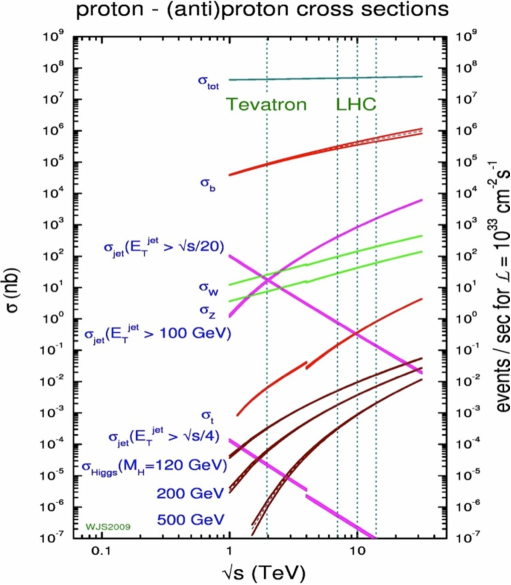
\includegraphics[width=0.55\textwidth]{images/cross-sections.png}
    \caption{Cross-sections for different processes at various collision energies as a function of center-of-mass energy \( \sqrt{s} \) \cite{cartiglia2013measurementprotonprotontotalelastic}.}
    \label{fig:crosssection}
\end{figure}

Central to particle tracking in the CMS Phase-2 upgrade detector is the Inner Tracker (IT) which will face enormous operational challenges as an extreme radiational exposure with a neutron equivalent fluence of up to $2.3 \times 10^{16}\text{n}_{eq}/\text{cm}^{2}$, a total ionizing dose (TID) reaching approximately $12\text{MGy}$ ($1.2 \text{Grad}$), and pixel hit rates as high as $3\text{GHz/cm}^{2}$ with up to 200 collisions per bunch crossing \cite{Apollinari:2284929, Malik:2816244}. To operate effectively under these harsh conditions, the upgraded detector must have improved spatial resolution, achieved through the reduced pixel size and sensor thickness, and electronics capable of high rates and enhanced radiation tolerance. The CMS Phase-2 upgrade is currently under development and testing at various international facilities, including Fermi National Accelerator Laboratory (FNAL), CERN, and German Electron Synchotron (DESY), to validate these technological advancements and ensure their robustness for HL-LHC operation.

At the FNAL Testbeam studies, silicon pixel sensors used as the Device Under Test (DUT) have been characterized in terms of cluster size and spatial resolution in the non-irradiated case. The pixel telescope resolution is utilized as the reference frame in determining the DUT resolution is approximately $10~\mu\text{m}$ and is attained through the integration of several layers of pixel planes.

When a charged particle traverses a silicon pixel sensor, it deposits energy and generates electron-hole pairs, following a Landau-like distribution in charge. In particular, particles that produce significantly higher than average charge are often associated with secondary interactions, such as delta-rays, which can complicate the reconstruction of the original particle trajectory. For this reason, it is relevant to study the pixel resolution, cluster size, and crosstalk as a function of the charge bins within the Landau distribution.

These studies not only provide a deeper understanding of sensor performance but also support a slight improvement of the telescope's resolution and allow for a more accurate determination of the DUT resolution. Chapters~3, 5 presents and discusses these investigations in detail.

Moreover, The HL-LHC upgrade will enhance the complexity and event rates, leading to a 7.5-fold rise in the readout rate \cite{Fernandez_Perez_Tomei_2020}. Currently, at the CMS experiment, event selection for further analysis is manually determined based on detector performance, particularly tracking. However, with the upgrade, the number of monitoring elements (MEs) will grow substantially, making manual decision-making both labor-intensive and prone to bias. Therefore, some automated tools capable of detecting unexpected or anomalous behavior will be highly beneficial. For this purpose, a Non-Negative Matrix Factorization (NMF) machine learning (ML) model is being explored as a possible approach. NMF enables dimensionality reduction of the input data to capture underlying patterns across Monitoring Elements (MEs), while reducing the reliance on manual inspection. So far, the model has been shown to successfully identify anomalies in synthetically generated data for one of the MEs. Chapters~4, 5 present and discuss this approach in detail.


\chapter{The CMS detector owerwiew}

%rewrite
The CMS detector is a multipurpose detector at the LHC. The detector layout is outlined in Figure \ref{fig:CMS_detector}. The detector consists of various sub-parts designed to measure different properties of the collision-produced particles. The closest to the interaction point (IP) is the tracker system, which operates within a 3.8 T magnetic field. Comprising pixel and strip detectors enables precise measurement of transverse momentum and positions of charged particles. In addition, reconstruction algorithms employed in the determination of the trajectories also yield fundamental information regarding single collisions, for instance, the impact parameter, which plays a critical role in displaced vertex identification and association to tracks for further sophisticated methods such as PU mitigation and flavor tagging.

\begin{figure}[h]
    \centering
    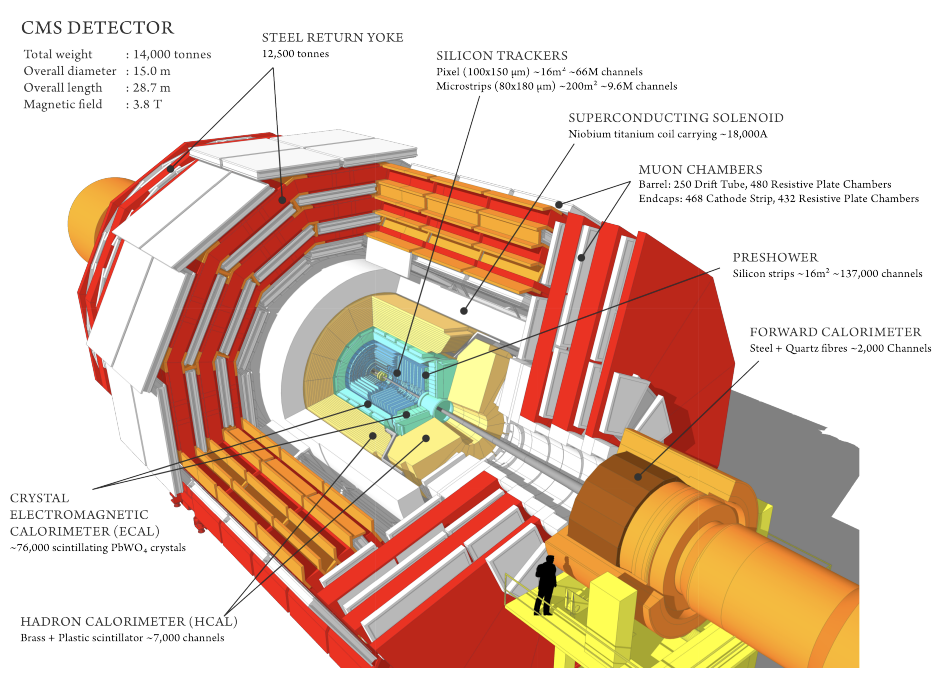
\includegraphics[width=0.9\textwidth]{images/CMS_detector.png}
    \caption{The CMS detector at the LHC \cite{Ghosh_2019}.}
    \label{fig:CMS_detector}
\end{figure}

The tracker system is followed by the electromagnetic (ECAL) and hadronic (HCAL) calorimeters. ECAL stops electromagnetically interacting particles, producing an electromagnetic shower as a result. That allows to measure the energy of these particles with high precision. HCAL has a similar principle of work but for hadrons, which are interacting strongly with absorber material. Some particles can pass calorimeters undetected, like neutrinos, for example, or just lose some energy, like muons. The presence of these particles can be detected by calculating reconstructed particles' momenta, also called missing transverse energy (MET). The calorimeters are crucial for jet reconstruction.

The outer part of the detector is the muon system, or muon chambers. Muons are distinguished by their minimal energy loss in the calorimeters and by matching tracks between the inner tracker and the muon system. Their momentum and position are measured there. Particles like neutrinos pass through the last layer of the detector without any interaction and can be detected only through MET \cite{The_CMS_Collaboration_2008, Hayrapetyan_2024}.

\section{Phase-2 Tracker Upgrade for the HL-LHC}

Phase-2 upgrade of the CMS detector is desighn to await the challenges facing the HL-LHC. Increase in luminosity by a factor of 5 and up to 200 bunch crossing collisions will expose the CMS tracking system to severe challenges, primarily due to high radiation levels and high density particle environment. The upgrade will include a new IT with a re-designed pixel detector with reduced pixel size, improved spatial resolution, and tracking capabilities. The current Phase-1 detector has pixel sizes of $100 \times 150~\mu\text{m}^2$, while the Phase-2 upgrade will include pixel sizes as small as $25 \times 100~\mu\text{m}^2$ in the barrel and $50 \times 50~\mu\text{m}^2$ in some forward regions (see Figure~\ref{fig:IT}), which supports a significant improvement in granularity \cite{thetrackergroupofthecmscollaboration2023evaluationplanarsiliconpixel, Orfanelli:2780125}.

\begin{figure}[H]
    \centering
    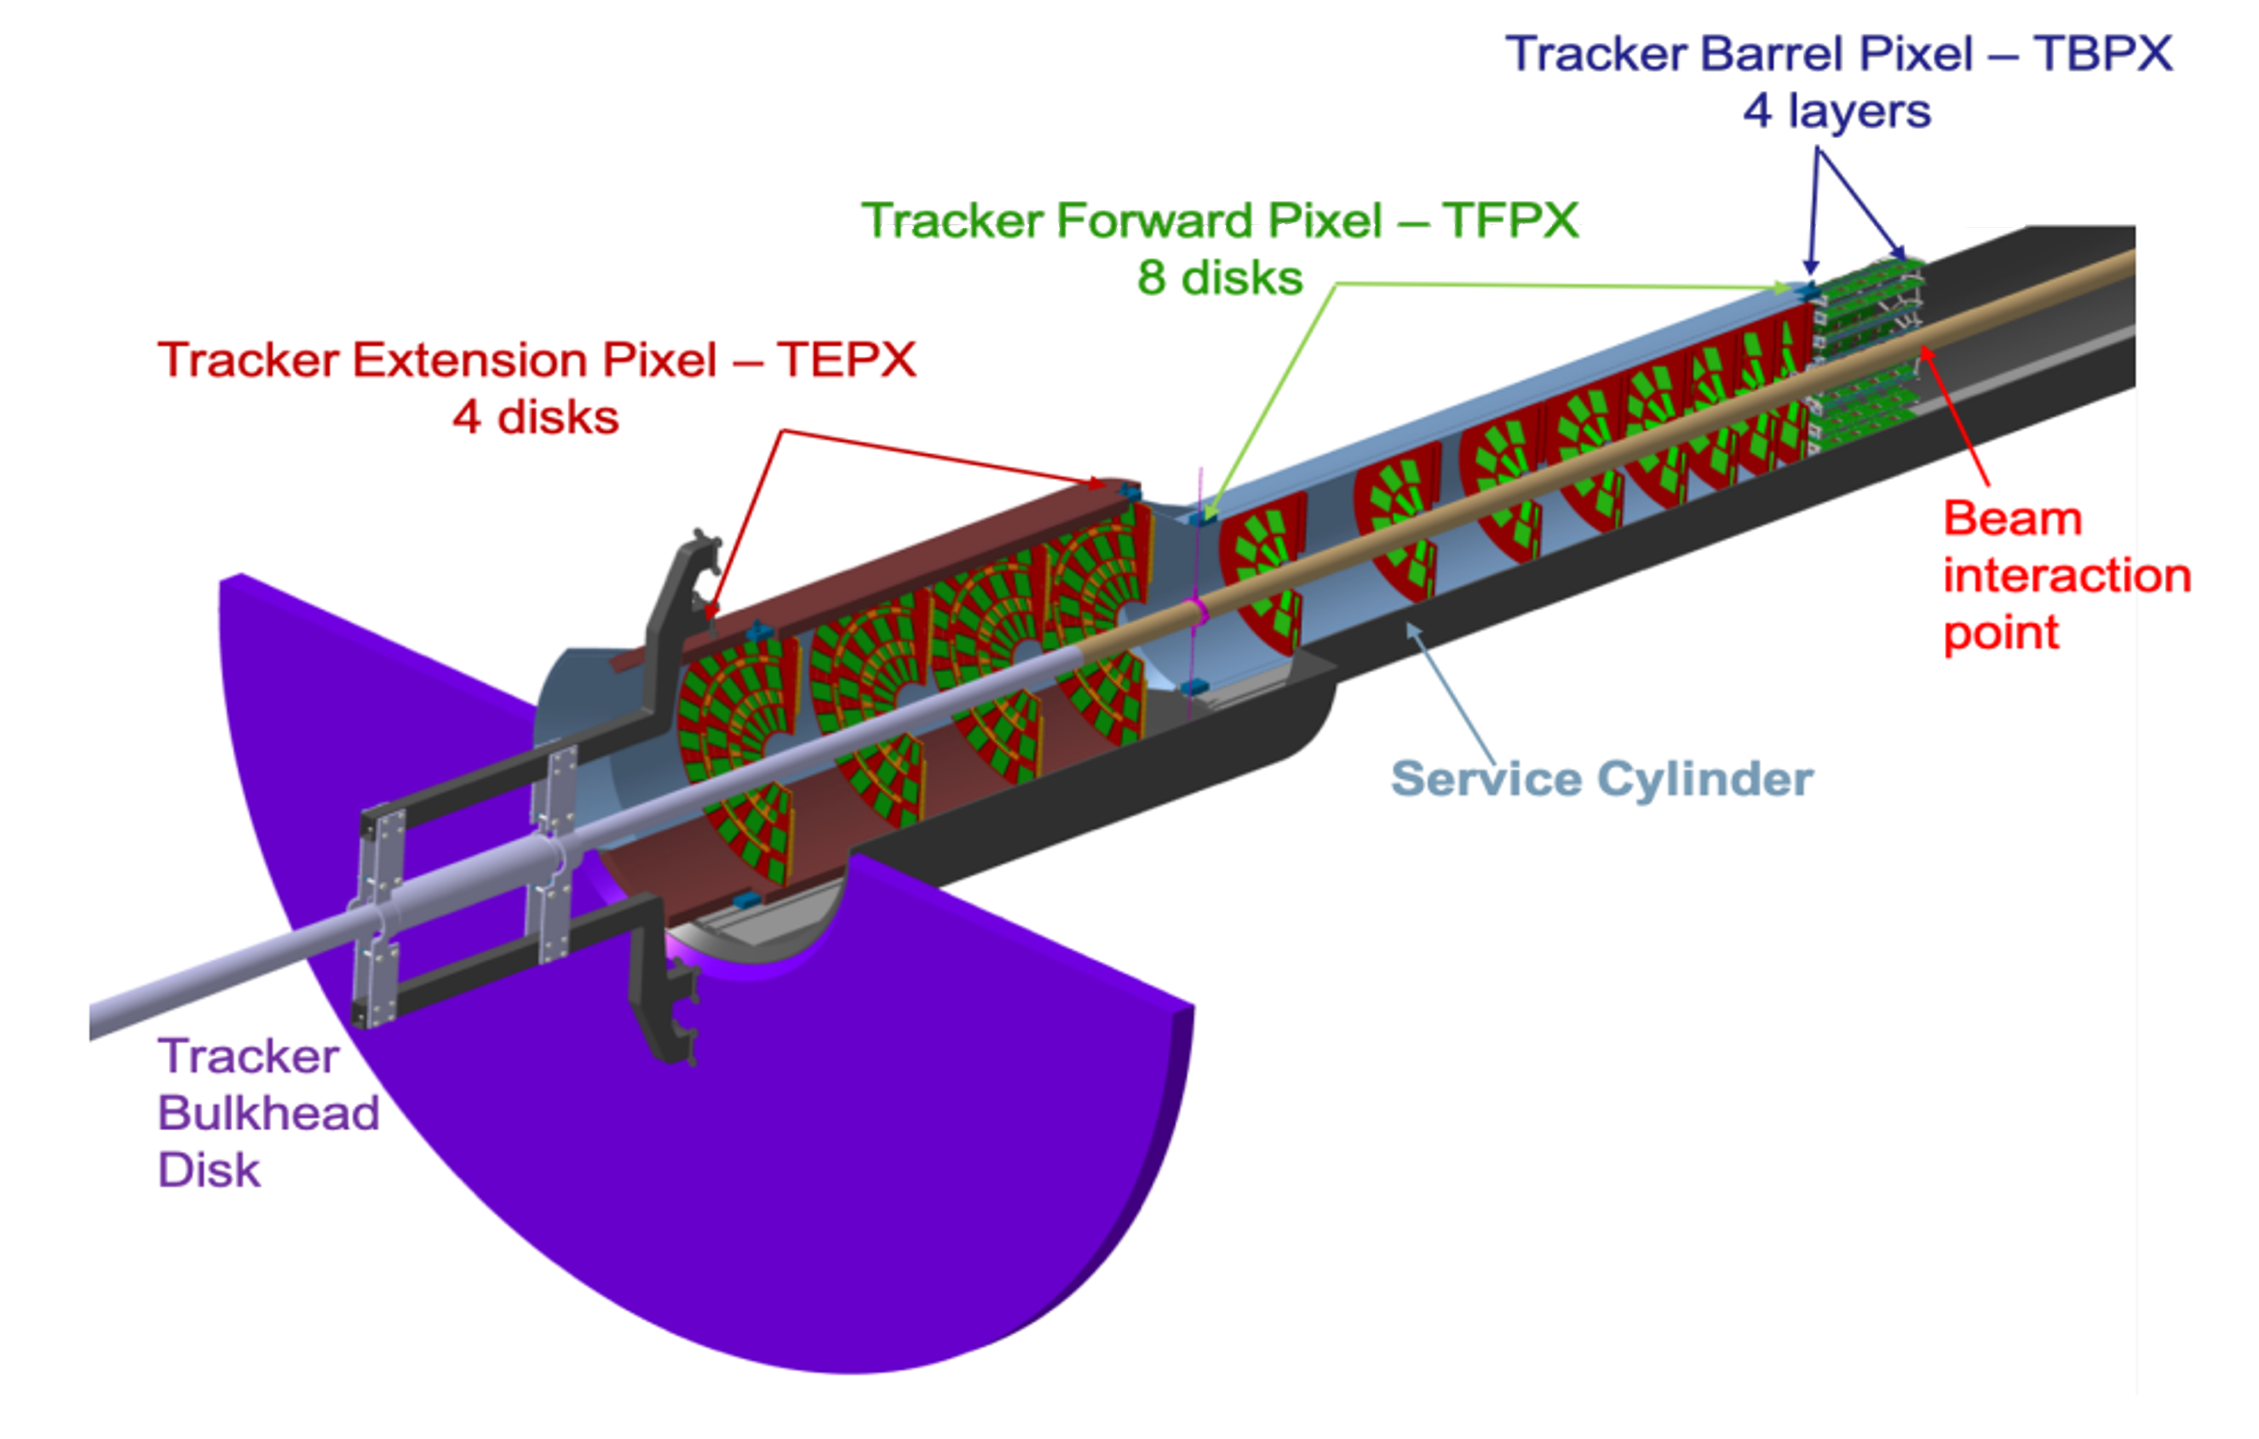
\includegraphics[width=0.8\textwidth]{images/IT.png}
    \caption{Exploded view of the CMS Phase-2 IT layout quarter, showing the Tracker Barrel Pixel (TBPX), the Tracker Forward Pixel (TFPX), and the Tracker Extension Pixel (TEPX).}
    \label{fig:IT}
\end{figure}

The Inner Tracker will consist of approximately two billion pixels, each with an area of $2500~\mu\text{m}^2$, arranged in modules with either two or four front-end readout chips, depending on their position. Two-chip modules are used in the inner barrel and the inner forward rings, while four-chip modules are employed in the outer barrel and outer forward regions, as shown in Figure~\ref{fig:tracking_layout}. This configuration enables tracking coverage up to $|\eta| \approx 4$, significantly improving the reconstruction of forward tracks and enhancing sensitivity to highly boosted or displaced signatures.

\begin{figure}[H]
    \centering
    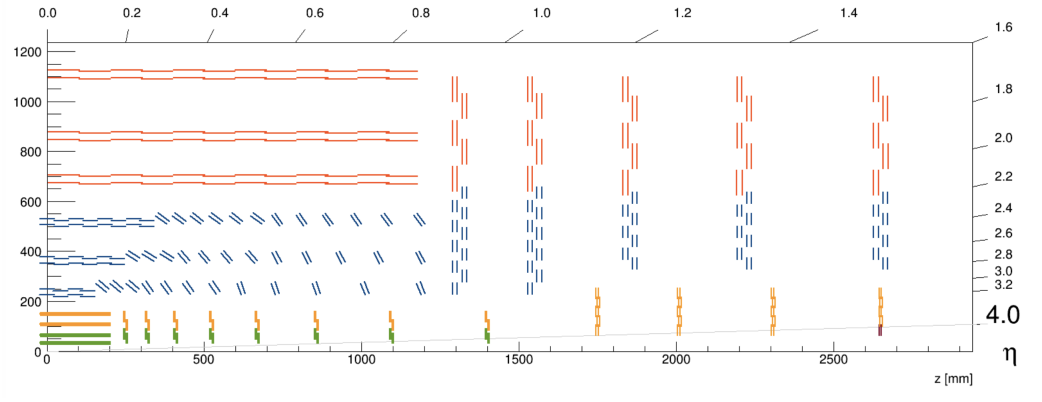
\includegraphics[width=1\textwidth]{images/tracker_layout.png}
    \caption{Sketch of one quarter of the CMS Phase-2 Tracker layout in the longitudinal ($z$--$r$) plane. Outer Tracker modules are shown in red (strip-only) and blue (pixel-strip), while Inner Tracker pixel modules are shown in green (double readout chip) and orange (quad readout chip). The $z$-axis runs along the beam direction, and the $r$-axis indicates the radial distance from the beamline. The right vertical axis shows the corresponding pseudorapidity ($\eta$) coverage, which extends up to $|\eta| \approx 4$ \cite{Outertracker}.}
    \label{fig:tracking_layout}
\end{figure}

The improved Inner Tracker is aimed at long-term functionality under severe radiation environments, with sensor modules having the ability to sustain fluences up to $2 \times 10^{16}~\text{n}_\text{eq}/\text{cm}^2$ \cite{Malik:2816244}. Moreover, it is anticipated to play a significant role in the Level-1 trigger system by providing quick tracking information essential to fast event selection. Whereas this emphasis is on the Inner Tracker, the Outer Tracker will give further coverage by utilizing strip-based 2S and PS modules, organized into six barrel layers and twelve endcap disks \cite{Outertracker}.

\section{Data Quality Monitoring of the Tracker System}

The function of the CMS detector is to reconstruct particles and events produced by proton-proton collisions. Naturally, none of the subdetectors performs ideally, and each measures physical properties with finite precision. As the Tracker system is the closest to the IP, its precise functioning is crucial to the reconstruction of primary and secondary vertices (PVs and SVs) and to obtaining better spatial resolution. It is thus imperative to ensure the optimal functioning of this system for reliable physics analyses and this needs to be supported by a strong framework for Data Quality Monitoring (DQM).


The tracker DQM infrastructure monitors the status and output of silicone pixels and strip detectors while taking frequent data. This includes checking for dead or noisy channels, assessing cluster properties, tracking efficiency, hit oxuency, alignment stability and other performance indicators. Data quality evaluation is done in real time during data-carry (online DQM), and in more detail in offline workflows after complete reconstruction (offline DQM). These assessments help identify hardware failures, calibration issues and unexpected discrepancies that can compromise data integrity.

Monitoring is performed through a large set of histogram and monitoring elements (MEs), conducted by detector components and trigger conditions. These are reviewed by trained shifters and experts using devices such as DQM graphical user interface (GUI) and DQM data certification interfaces (see Figure~\ref{fig:dqm_gui}). For tracker, this process is especially important due to its complexity and sensitivity to operating conditions such as temperature, magnetic field and radiation-inspired damage \cite{DQM_1, DQM_2}.

In recent years, efforts have been made to automate parts of the DQM process using machine learning (ML) techniques, especially in the preparation of the high-luminosity LHC (HL-LHC) era, where the data volume will increase significantly. The purpose of these efforts is to detect discrepancy, reduce human workload and ensure timely identification of possible issues in the tracker system.

\begin{figure}[H]
    \centering
    \begin{subfigure}[t]{1\textwidth}
        \centering
        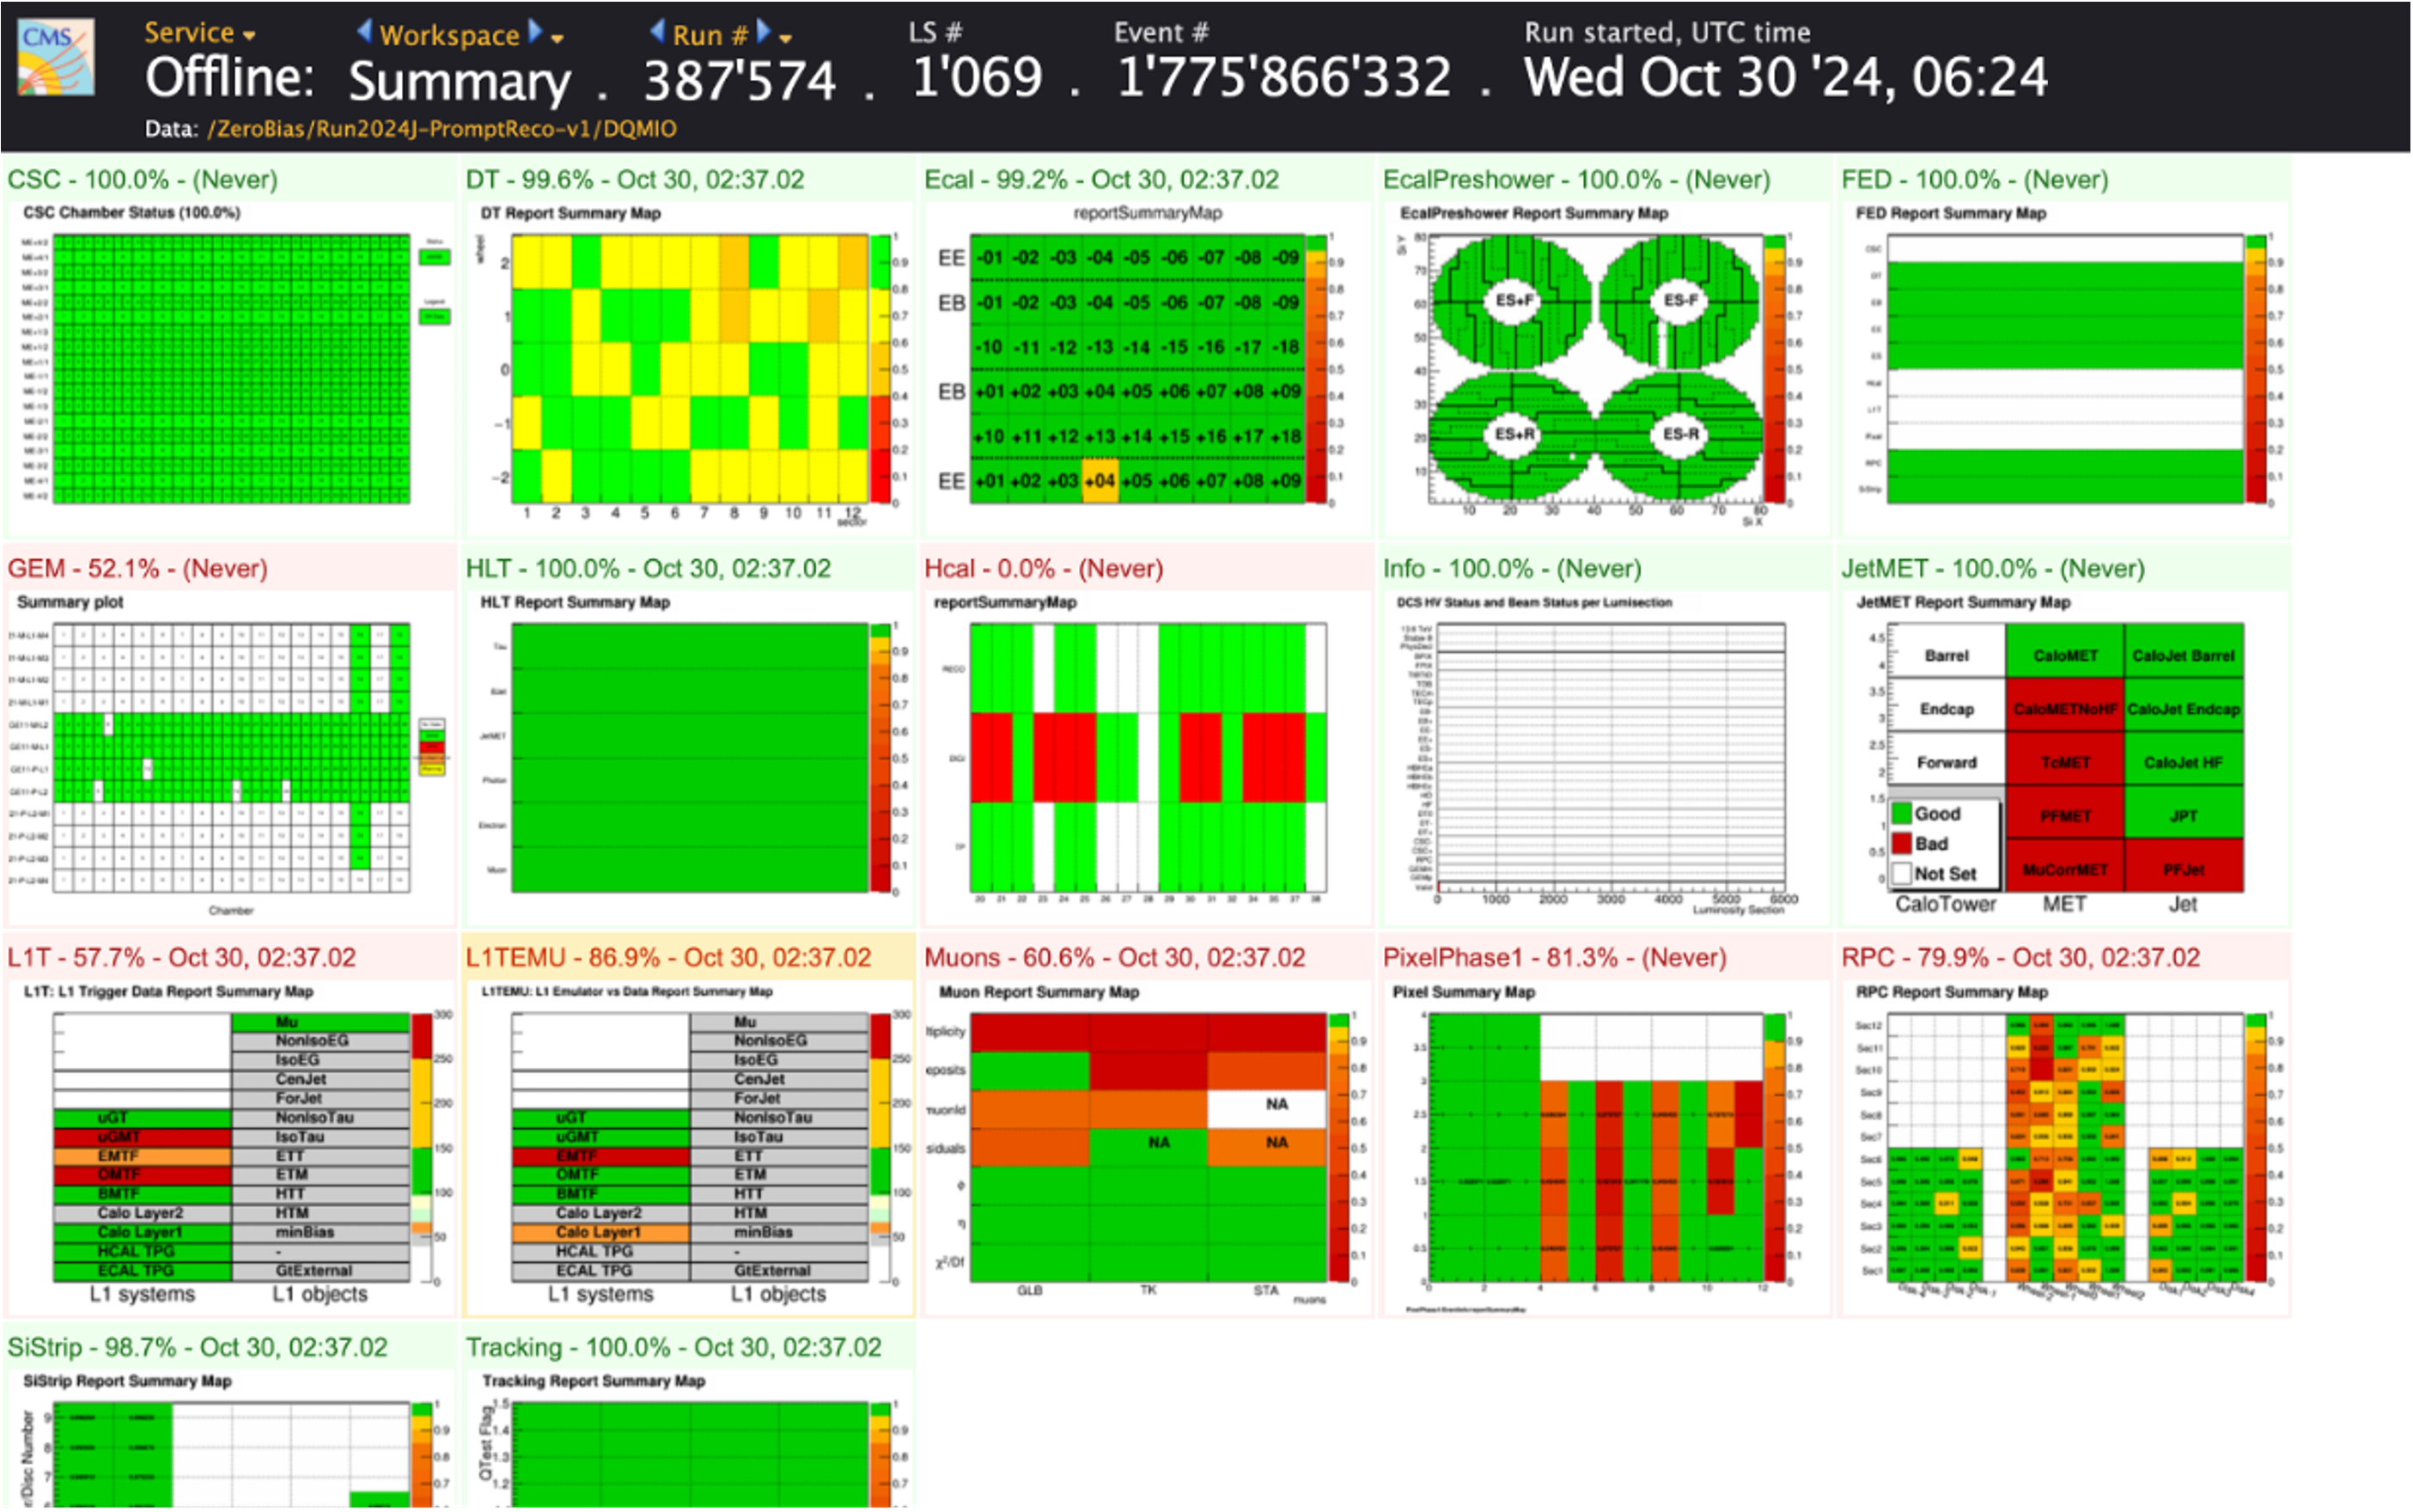
\includegraphics[width=\textwidth]{images/dqm_gui.png}
        \label{fig:dqm_gui_1}
        \caption*{(a)} % Manual label only
    \end{subfigure}

    \vspace{1em}

    \begin{subfigure}[t]{1\textwidth}
        \centering
        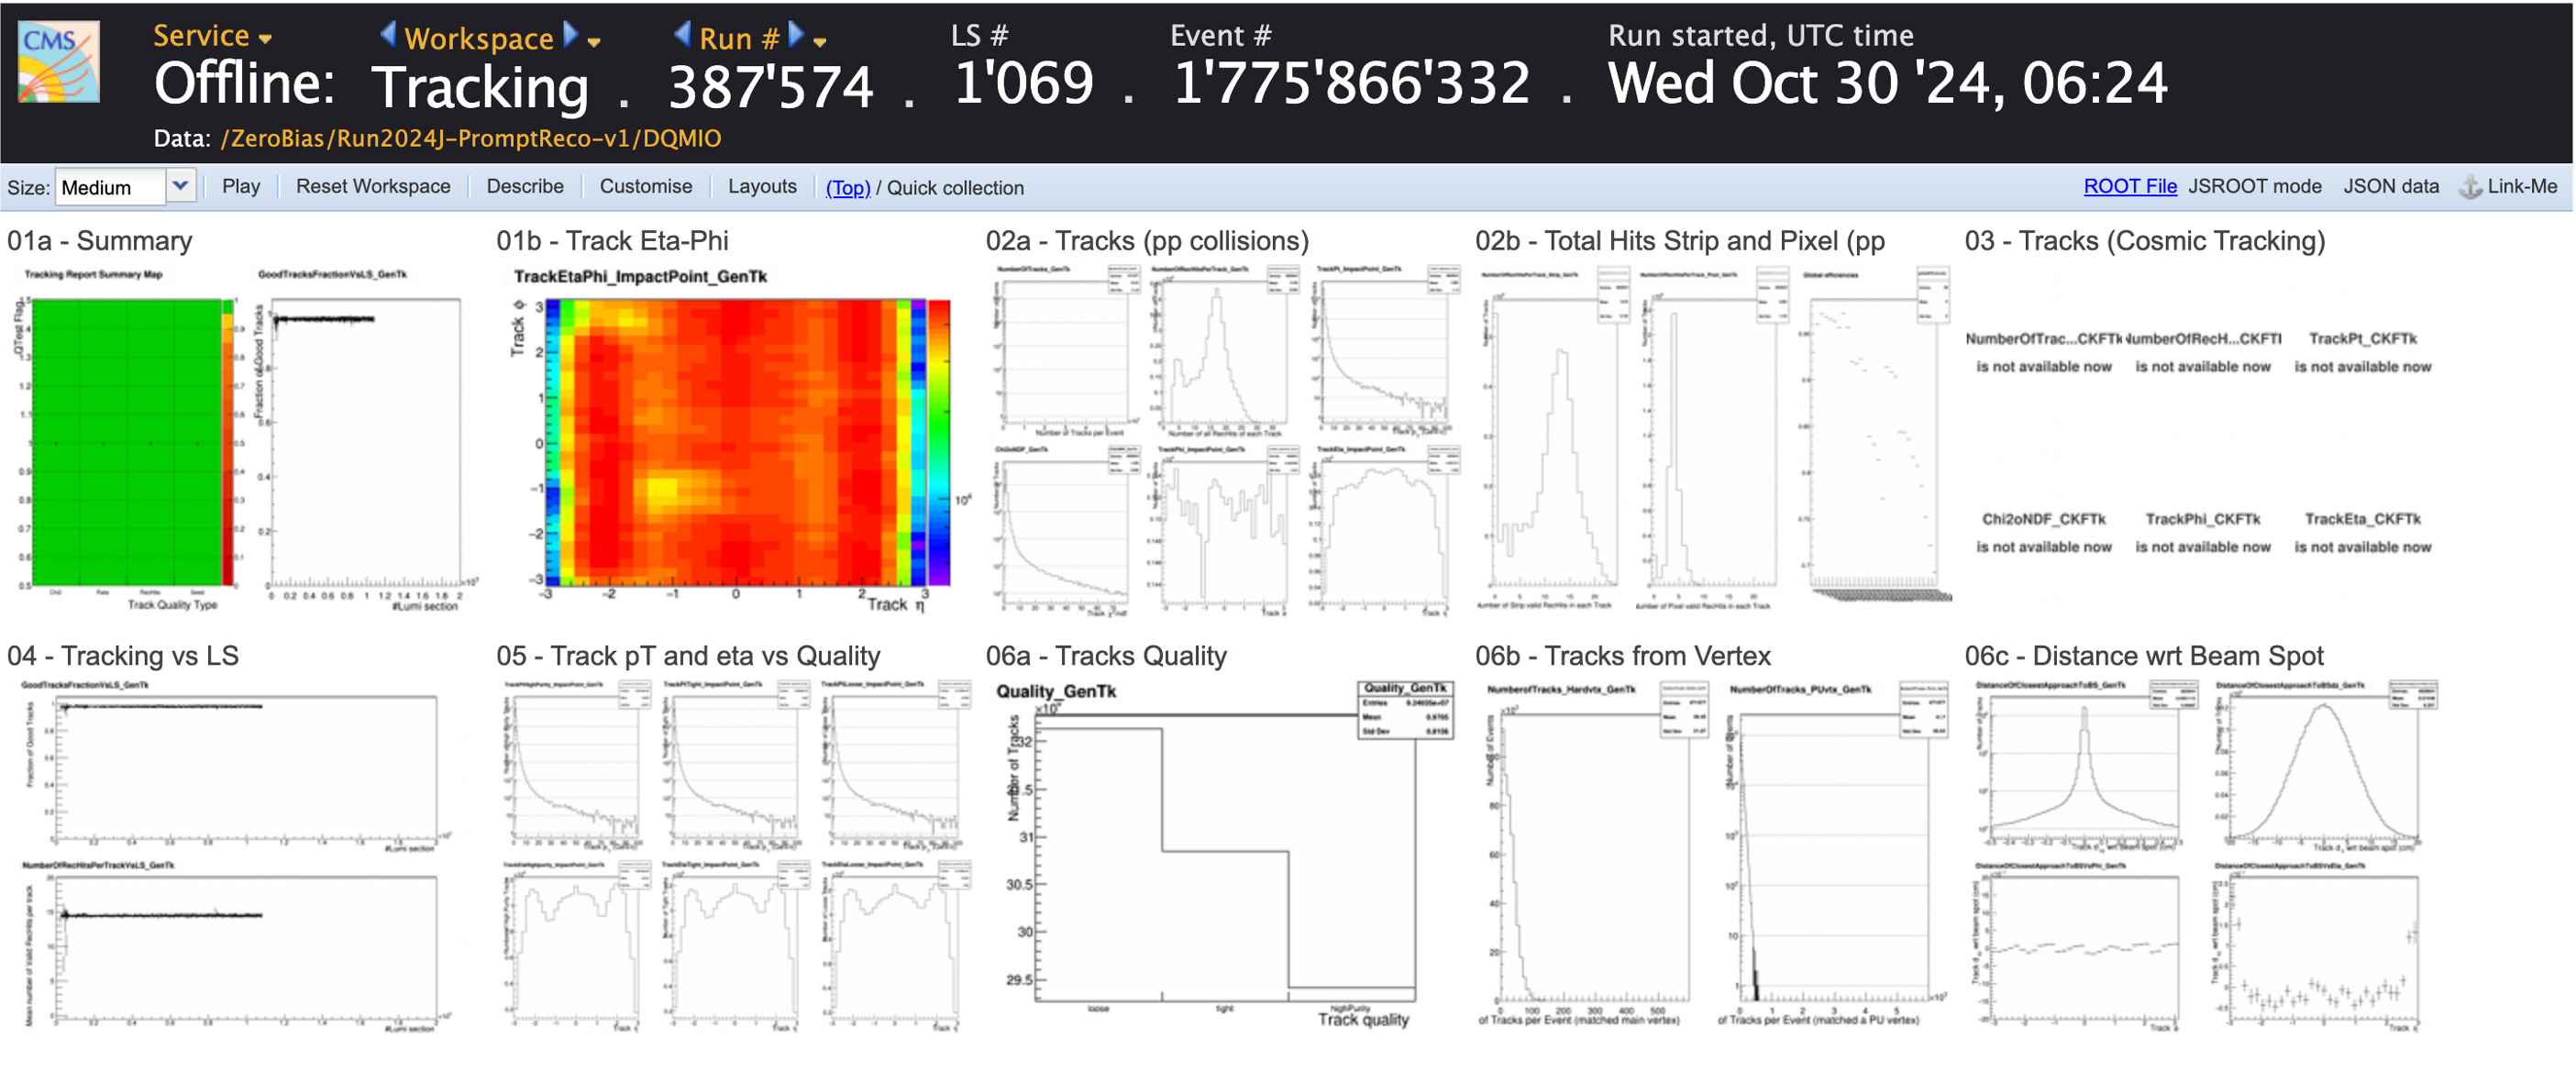
\includegraphics[width=\textwidth]{images/gui_tracker.png}
        \label{fig:dqm_gui_2}
        \caption*{(b)} % Manual label only
    \end{subfigure}

    \caption{A snapshot of the Offline DQM GUI displaying the global summary view (a), and a detailed view of MEs for the tracking system (b).}
    \label{fig:dqm_gui}
\end{figure}

\chapter{Testbeam experiment at FNAL}

Testbeam experiment provides a controlled environment in which detectors are exposed to particle beams that mimics real experimental conditions. The experiment is required for evaluating the performance of prototype detector modules prior to their installation in large-scale experiments such as CMS. The following sections present the beam facility, experimental configuration and key physics considerations relevant to the study.

\section{The Fermilab Test Beam Facility}

The Fermilab Test Beam Facility (FTBF), located in Batavia, Illinois, is a high-energy accelerator facility dedicated to testing and developing particle detectors for experiments such as CMS. It delivers a primary beam of $120\,\text{GeV}$ protons at variable intensities (1--300\,kHz), extracted in controlled spills approximately every 60 seconds.

The beam is formed by a sequence of accelerators: $750\,\text{keV}$ H$^-$ ions are first accelerated initially in the Linear Accelerator (Linac) to $400\,\text{MeV}$, then injected into the Booster where electrons are stripped and protons are accelerated to $8\,\text{GeV}$. These protons are transferred to the Main Injector and boosted to $120\,\text{GeV}$. The extracted beam is then routed through the Fermilab Switchyard, which splits and directs it to experimental areas, including the Meson Test Beam Facility (MTest) and the Meson Center Beam Facility (MCenter). Secondary and tertiary beamlines can also be created by placing absorbers and targets into the primary beamline. These consist of muons, pions, or electrons, with energies as low as $1\,\text{GeV}$ for the secondary beamline and down to $200\,\text{MeV}$ for the tertiary beamline. A schematic of the beamline is shown in Figure~\ref{fig:fermi_complex}.

\begin{figure}[H]
    \centering
    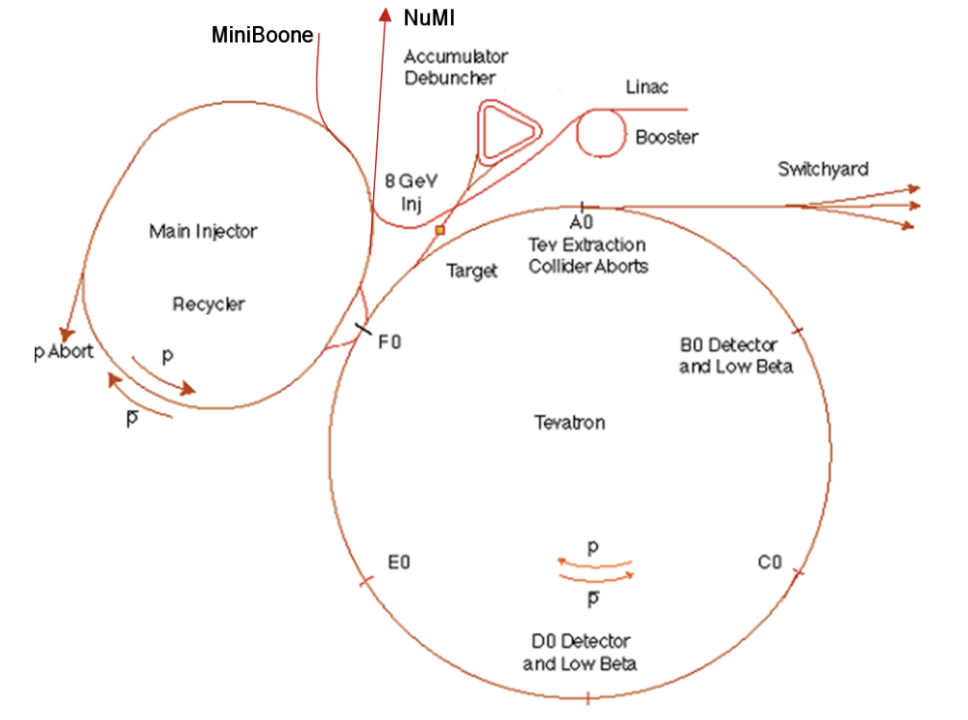
\includegraphics[width=0.8\textwidth]{images/Fermilab_accelerator.png}
    \caption{Schematic layout of the Fermilab accelerator complex \cite{Stephen_Holmes_2011}.}
    \label{fig:fermi_complex}
\end{figure}

A silicon pixel tracking telescope is permanently installed in MTest to provide high-resolution tracking of beam particles Fermilab also hosts the Irradiation Test Area (ITA), which is used for controlled radiation studies of detector components under HL-LHC-like conditions.

\section{Telescope Infrastructure and Alignment}

The tracking telescope at FNAL is designed to sustain high-precision measurements of the Device Under Test (DUT). The telescope includes six silicon strip planes positioned upstream, where two pairs of planes are arranged orthogonally to each other to improve resolution by measuring the X and Y positions of hits. Downstream of the DUT, four pixel planes are placed together with the same six strip planes, as shown in Figure~\ref{fig:telescope}. The pixel sensors employ $100 \times 150 \times 320~\mu\text{m}^3$ cells and cover an active area of approximately $1.6 \times 1.6~\text{cm}^2$, achieving a resolution of about $8~\mu\text{m}$ due to the tilted sensor geometry. The strip detectors provide even better resolution, approximately $5~\mu\text{m}$, with a pitch of $60~\mu\text{m}$ and an active area on the order of $3.8 \times 3.8~\text{cm}^2$ \cite{KWAN2016162}.

\begin{figure}[H]
    \centering
    \includegraphics[width=1\textwidth]{images/telescope.png}
    \caption{FNAL telescope structure.}
    \label{fig:telescope}
\end{figure}

The primary beam within the MTest area traverses three scintillators placed upstream and one scintillator downstream of the pixel telescope. The coincidence of these scintillators creates a signal that starts the data acquisition for the entire detector arrangement. A unique identifier is assigned to each trigger so that data from the pixel planes, strip detectors, and DUT possible be arranged into a single unit referred to as an "event". Track reconstruction up to frequencies of about 40 kHz is supported by the system while maintaining trigger information integrity. In addition to trigger numbers, timestamps are saved to allow offline synchronization of the telescope and DUT data streams.

Data acquisition is controlled by the Compact And Programmable daTa Acquisition Node (CAPTAN), a system developed at Fermilab \cite{Adam_2019}. The telescope consists of three independent stations, each containing a CAPTAN module. The central module, which is also connected to the DUT, mantained as the master module and synchronizes data taking in the whole system. All modules are linked to the control room computer, where data is recorded and monitored over the operational time.

Telescope alignment is performed offline using the Monicelli program. It begins with the reconstruction of tracks using a chi-squared fit of the hit positions, with cluster positions given by charge-weighted averages if there are multiple pixels. Monicelli then iteratively adapts the telescope geometry to minimize the residuals in the transverse directions for each pixel plane. The optimal geometry, characterized by the minimum residuals, is selected. This arrangement, together with the fixed position of the DUT, allows the beam position at the DUT to be determined correctly.

\section{Planar sensor structure and physics properties}

The Testbeam experiment's planar silicon sensors are produced by Hamamatsu Photonics K.K. (HPK) and are tested as a component of the DUT within the telescope setup. The sensors are intended to be bump-bonded with CMS Readout Chips (CROCs). Two pixel sensor dimensions, to be standardized for the HL-LHC, are presented in Figure~\ref{fig:pixel_sensors}.

\begin{figure}[H]
    \centering
    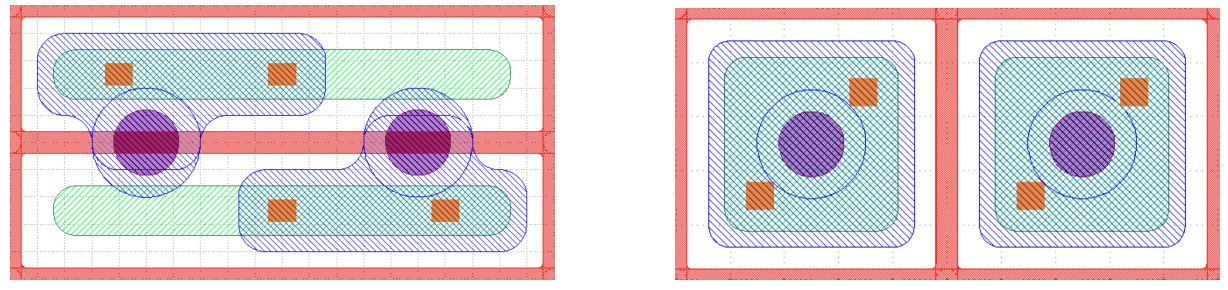
\includegraphics[width=1\textwidth]{images/pixels.png}
    \caption{Layout of two pixel cells of the HPK sensor submission: $25 \times 100~\mu\text{m}^2$ (left) and $50 \times 50~\mu\text{m}^2$ (right). The $n^+$ implants are shown in green, metal layers in blue, $p$-stop regions in red, contacts in orange, and bump bond pads in purple \cite{CERN-LHCC-2017-009}.}
    \label{fig:pixel_sensors}
\end{figure}

Silicon semiconductors are fundamental for particle detectors due to the small band gap which allow ionization radiation such as a MIP to remove electrons from valence zone generating electron-hole pairs and typically deposits around 80 $e$--$h$ pairs per micrometer of sensor thickness.

\begin{figure}[H]
    \centering
    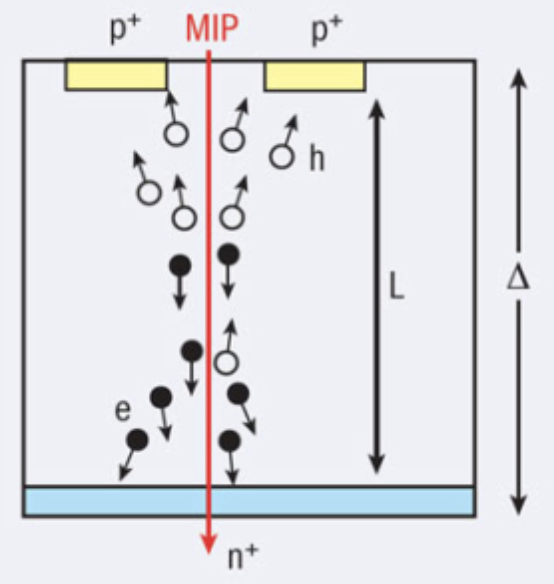
\includegraphics[width=0.4\textwidth]{images/planar_sensor.png}
    \caption{Schematic cross-section of a planar sensor design, illustrating how the active thickness ($\Delta$) and the charge collection distance ($L$) are independently defined.}
    \label{fig:planar_sensor}
\end{figure}

When a reverse bias voltage ($V_{\text{bias}}$) is applied across the $p^+$--$n^+$ junction, it depletes the free charge carriers from the bulk of the sensor, generating an electric field $\vec{E}$ which extends into the active thickness $\Delta$. When the depletion region extends throughout the entire sensor, the sensor becomes fully depleted. The drift of the holes and electrons under the influence of the electric field induces a current, which is picked up by the readout chips. The total charge $Q$ from a traversing particle can be estimated by:
\begin{equation}
    Q = q \cdot \frac{dE}{dx} \cdot \Delta,
\end{equation}
where $q$ is the elementary charge, $dE/dx$ s the particle's energy loss per unit path length. Its variation with the momentum of the particle is given by the Bethe-Bloch equation, which is plotted in Figure~\ref{fig:Bloch}. The curve indicates how the stopping power of charged particles changes with their energy and drops to a minimum value known as minimum ionization. Most particles formed by high-energy collisions pass through silicon sensors in this regime, releasing a very uniform amount of energy, and thus the response of the detector is known and reproducible.

For optimum performance, the sensor is biased slightly above full depletion in order to reduce the leakage current and prevent breakdown. Leakage current rises with voltage as:
\begin{equation}
    I_{\text{leak}} \propto \sqrt{V_{\text{bias}}},
\end{equation}
up to full depletion, then rising steeply, at which breakdown begins.

Figure~\ref{fig:planar_sensor} is a schematic of a planar sensor geometry with an MIP generating $e$--$h$ pairs, which are subsequently separated by the electric field and collected at the opposite electrodes, inducing a detectable signal.

\begin{figure}[H]
    \centering
    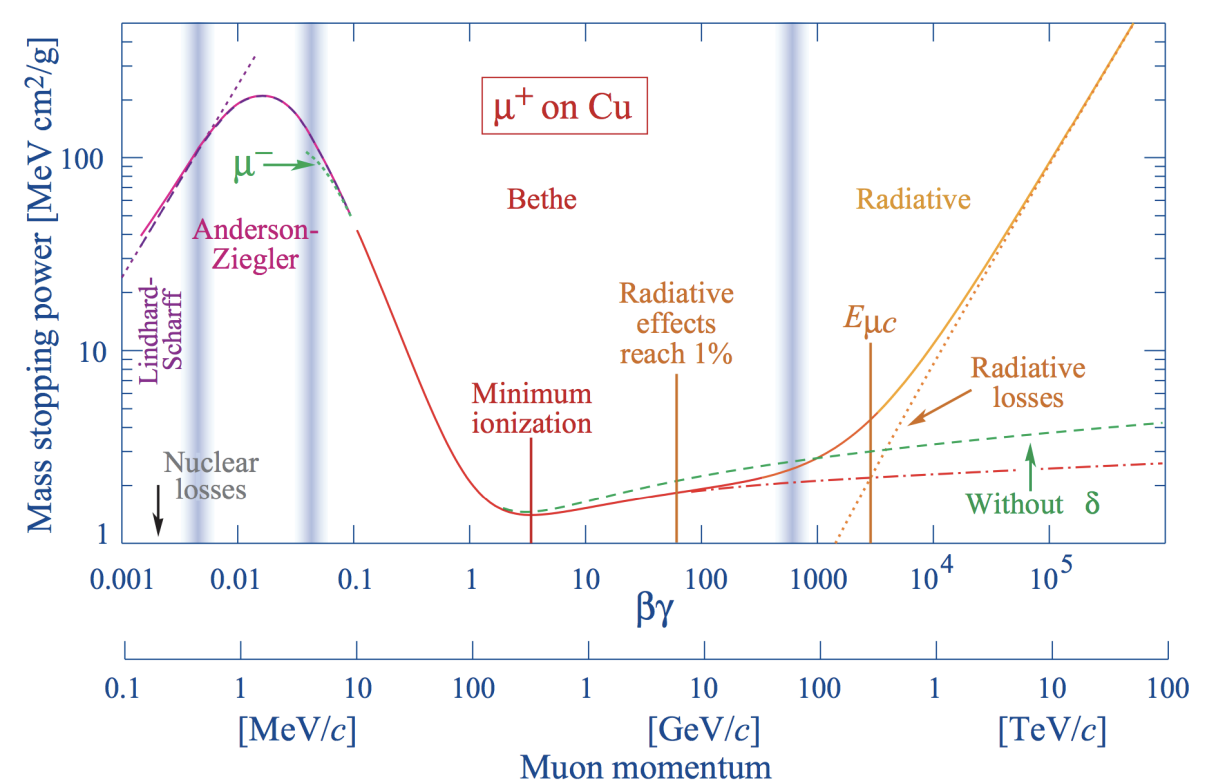
\includegraphics[width=0.9\textwidth]{images/Bloch.png}
    \caption{Mass stopping power ($-\frac{dE}{dx}$) for muons in copper as a function of $\beta\gamma = \frac{p}{mc}$ (bottom axis) and momentum (top axes), showing the Bethe-Bloch behavior. The curve is a plateau at minimum ionization, rising at high energy from radiative losses. This behavior produces the minimum ionizing particles (MIPs) energy loss in silicon-based tracking detectors \cite{Bichsel200827PO}.}
    \label{fig:Bloch}
\end{figure}

\section{Sensor Response Effects}
\subsection{Radiation Damage}

The radiational damage of silicon sensors is critical for the efficiency of the detector for the HL-LHC. The damage may take the form of crystal lattice defects (bulk damage) or surface damage due to interactions with insulating layers. These effects result in higher leakage currents, deformation of the electric field distribution, and charge trapping—all resulting in inefficient charge collection. Furthermore, radiation damage will raise the electronic noise, which can be partly eliminated by selecting a suitable readout threshold \cite{Eber_2014}.

\subsection{Charge Charing}

When a charged particle (such as a MIP) traverses a silicon sensor, it produces electron-hole pairs along its trajectory. The charge carriers are subsequently separated and drift under the influence of an electric field toward the collecting electrodes. If the particle passes near the boundary between two neighboring pixels, the resulting charge cloud may spread due to diffusion—particularly in the transverse direction—or be displaced by Lorentz drift in the presence of a magnetic field. As a result, both electrodes may collect a portion of the charge, leading to what is known as charge sharing.

\subsection{Crosstalk}

Crosstalk is the result of unintentianal signal coupling between adjacent pixels which leads to a degradation of the spatial resolution and misreconstruction of hits.

In Figure~\ref{fig:xtalk_layout}, a top perspective of a pixel layout demonstrates coupling between metal lines of neighboring pixels which is a common source of capacitive crosstalk.

\begin{figure}[H]
    \centering
    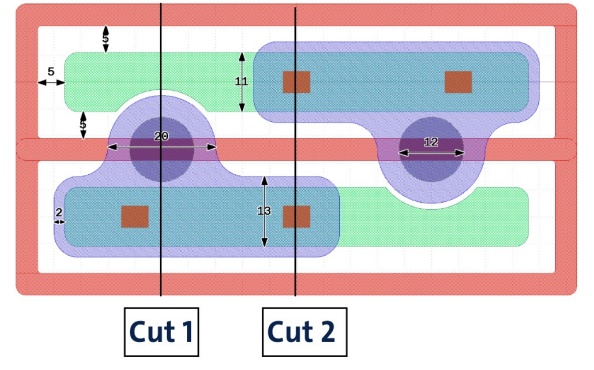
\includegraphics[width=0.5\textwidth]{images/RH0017.png}
    \caption{Top view of the pixel cell layout showing n$^+$ implants (green), metal lines (blue), p-stop structures (red), and passivation layers. The proximity of metal traces across neighboring pixels can give rise to capacitive crosstalk.}
    \label{fig:xtalk_layout}
\end{figure}

Figure~\ref{fig:xtalk_cut} illustrates vertical cuts (Cut 1 and Cut 2) of the pixel cell structure. The lack of any type of shielding or isolation structures in steps as such may result in a signal going through one pixel coupling to the neighboring pixel.

\begin{figure}[H]
    \centering
    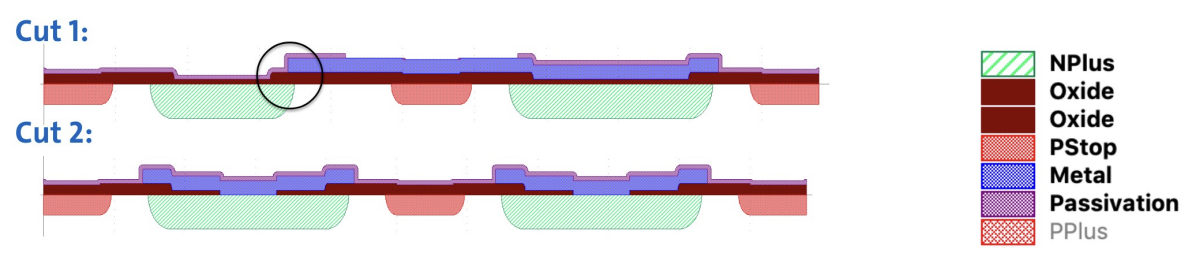
\includegraphics[width=0.8\textwidth]{images/RH0017cut.png}
    \caption{Cross-sectional views (Cut 1 and Cut 2) of the pixel sensor illustrating different vertical layouts. In Cut 1 the metal layer can increase capacitive coupling between adjacent pixels, leading to crosstalk.}
    \label{fig:xtalk_cut}
\end{figure}

Good shielding and layout practices are needed to minimize crosstalk.

\subsection{Delta rays}

Delta rays are secondary electrons of high energy knocked out of atoms during irradiation by a fast charged particle. They shift far from the parent track and generate further ionization, creating electron-hole pairs on trajectories other than the central one. The charge deposition can thus extend to the adjacent pixels, causing more charge sharing and in general forming larger or asymmetrical clusters. The photons can additionally distort charge patterns and complicate track reconstruction, particularly in high-precision pixel detectors.

\chapter{Tracker DQM}

Maintaining the integrity of the tracking performance of the collected data is foundational. The current monitoring process is handled manually by people. With the HL-LHC upgrade, the number of MEs and event rates will increase significantly, which will make the manual process even harder. The NMF approach can be used to automate some of these processes for anomaly detection.

\section{NMF-Based Model for Anomaly Detection}

NMF is a dimensionality reduction technique that factorizes input matrix \( X \in \mathbb{R}_{\geq 0}^{m \times n} \) into two lower-dimensional non-negative matrices: a coefficient matrix \( W \in \mathbb{R}_{\geq 0}^{m \times r} \) and a basis matrix \( H \in \mathbb{R}_{\geq 0}^{r \times n} \), such that:

\begin{equation}
    X_{m,n} \approx \sum_{r=1}^{k} W_{m,r} H_{r,n}
\end{equation}

Here, \( r \) is the number of components or latent features. The input matrix \( X \) represents histograms for a particular ME per LS, for example, charge distribution or cluster size. The rows of the matrix \( H \) represent the basis histograms, while \( W \) contains the weights corresponding to each feature used for reconstructing the data. During the training process, the Frobenius norm is used as an error for minimizing the difference between the input and reconstructed data:

\begin{equation}
    \min_{W, H \geq 0} \| X - WH \|_F^2
\end{equation}

After the basis matrix \( H \) and coefficient matrix \( W \) have been trained, test data \( X_{\text{test}} \) can be found in the same basis:

\begin{equation}
    W_{\text{test}} = \arg \min_{W \geq 0} \| X_{\text{test}} - WH \|_F^2
\end{equation}

The first component extracts dominant trends of the input data, and the remaining components extract variations, shifts in the distributions, noise, or handle the reconstruction of the tail of the Landau-like distribution. If the secondary components (all except the first one) have large contributing weights, or if the reconstruction error is significant, then the LS is anomalous.

Such anomalies may stem from a variety of sources, including:
\begin{itemize}
    \item Failing pixels or ROC-related issues,
    \item Trigger rate fluctuations,
    \item Synchronization problems within the Tracker readout system,
    \item Loss of hits or incomplete event data,
    \item and other detector or DAQ-related irregularities.
\end{itemize}


\chapter{Results}

\subsection{Charge Bin studies}

All of the studies were performed on the RH0017 module, which is a $1 \times 2$ CROC module with an HPK bias-dot $100 \times 25~\mu\text{m}^2$ sensor, where the shorter pitch corresponds to the $Y$ direction and the longer to the $X$ direction. The sensor layout has already been shown in Figure~\ref{fig:xtalk_layout}. The sensor is planar and non-irradiated. During data taking, the module was operated using chiller cooling only, following damage to the cold box due to a Peltier temperature excursion. The high-voltage bias was set to $-100$\,V. All the presented data correspond to a threshold of 1000 electrons.

The main purpose of the charge Bin studies is to better understand the effect of delta rays on the DUT and telescope resolution. If the effect is noticeable and significant, it could justify excluding such tracks from the general alignment procedure. This could potentially improve the telescope alignment by removing tracks associated with secondary particle production, which degrade the precision of the data.

The charge distribution is typically Landau-like, with delta-ray tracks contributing to the high-charge tail of the distribution. More specifically:
\begin{itemize}
    \item \textbf{Bin 3 (Low charge)}: $0 < Q \leq 0.85\,Q_a$
    \item \textbf{Bin 2 (Below average)}: $0.85\,Q_a < Q \leq Q_a$
    \item \textbf{Bin 1 (Above average)}: $Q_a < Q \leq 1.5\,Q_a$
    \item \textbf{Bin 0 (High charge / delta-ray candidates)}: $Q > 1.5\,Q_a$
\end{itemize}
\noindent
where \( \mathbf{Q_a} \) denotes the mean (average) detected charge across all clusters or see the Figure~\ref{fig:charge_bins}.

\begin{figure}[H]
    \centering
    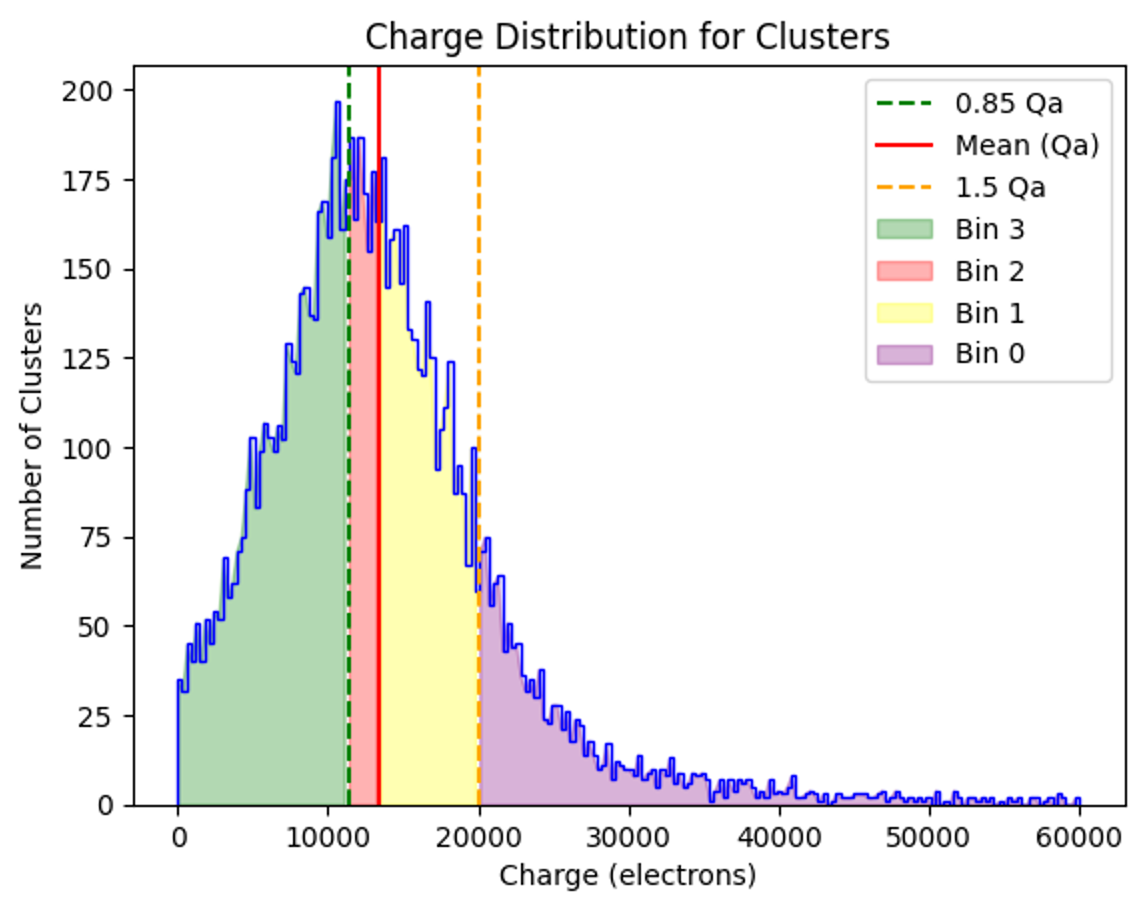
\includegraphics[width=0.7\textwidth]{images/Bins.png}
    \caption{Representation of the studied charge Bins with respect to \( Q_a \), the mean detected charge.}
    \label{fig:charge_bins}
\end{figure}

Resolution for the clusters of cluster size 2 is always superior to that for the clusters of other cluster sizes due to charge sharing. In this way, the track was traversing the DUT closer to the pixel edge, and the predicted position difference is smaller than when detected anywhere within even 1 pixel. It is also expected that for lower charge Bins (delta-ray candidates), the clusters formed are larger than for other charges, which will lead to having more clusters with large cluster sizes, like in Bin 0. Thus, comparing the residual distributions for cluster size 1 and cluster size 3 was considered to be helpful. The results obtained are presented in Figure~\ref{fig:resolution_size_1&3}. The residual is then approximated on all the planes of the telescope, with measurements taken using the DUT. Intuitively, the residual for cluster size 1 should be better, and this was confirmed by the results, even though the difference is not as significant.

\begin{figure}[H]
    \centering
    \begin{subfigure}[t]{0.485\textwidth}
        \centering
        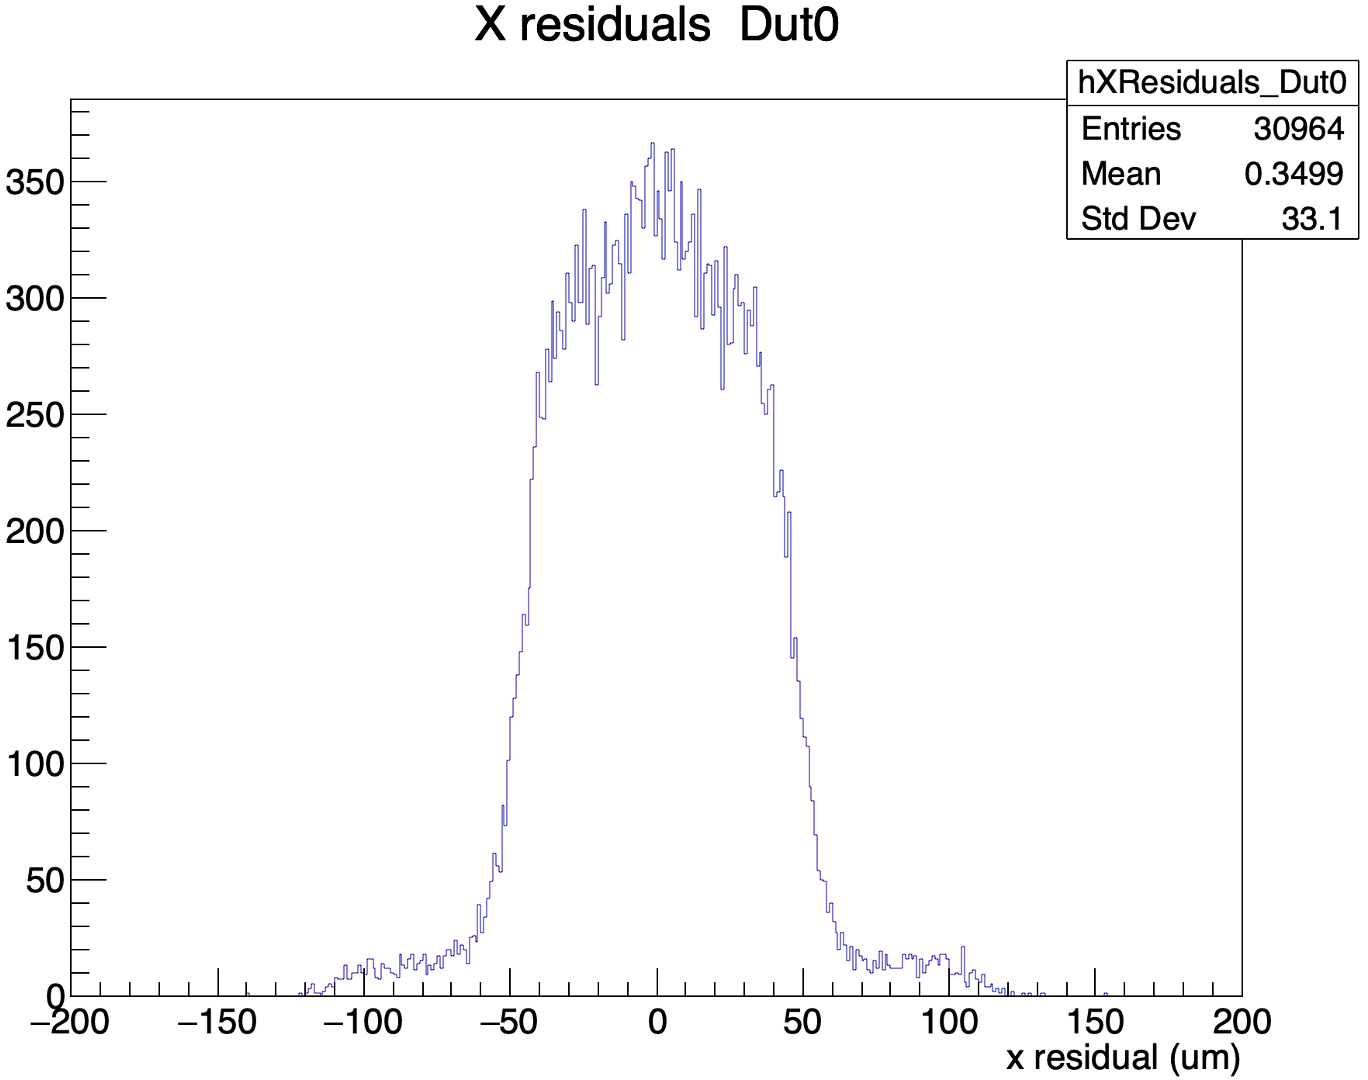
\includegraphics[width=\textwidth]{images/XRes_13planes.png}
        \caption{}
        \label{fig:dist_a}
    \end{subfigure}
    \hfill
    \begin{subfigure}[t]{0.45\textwidth}
        \centering
        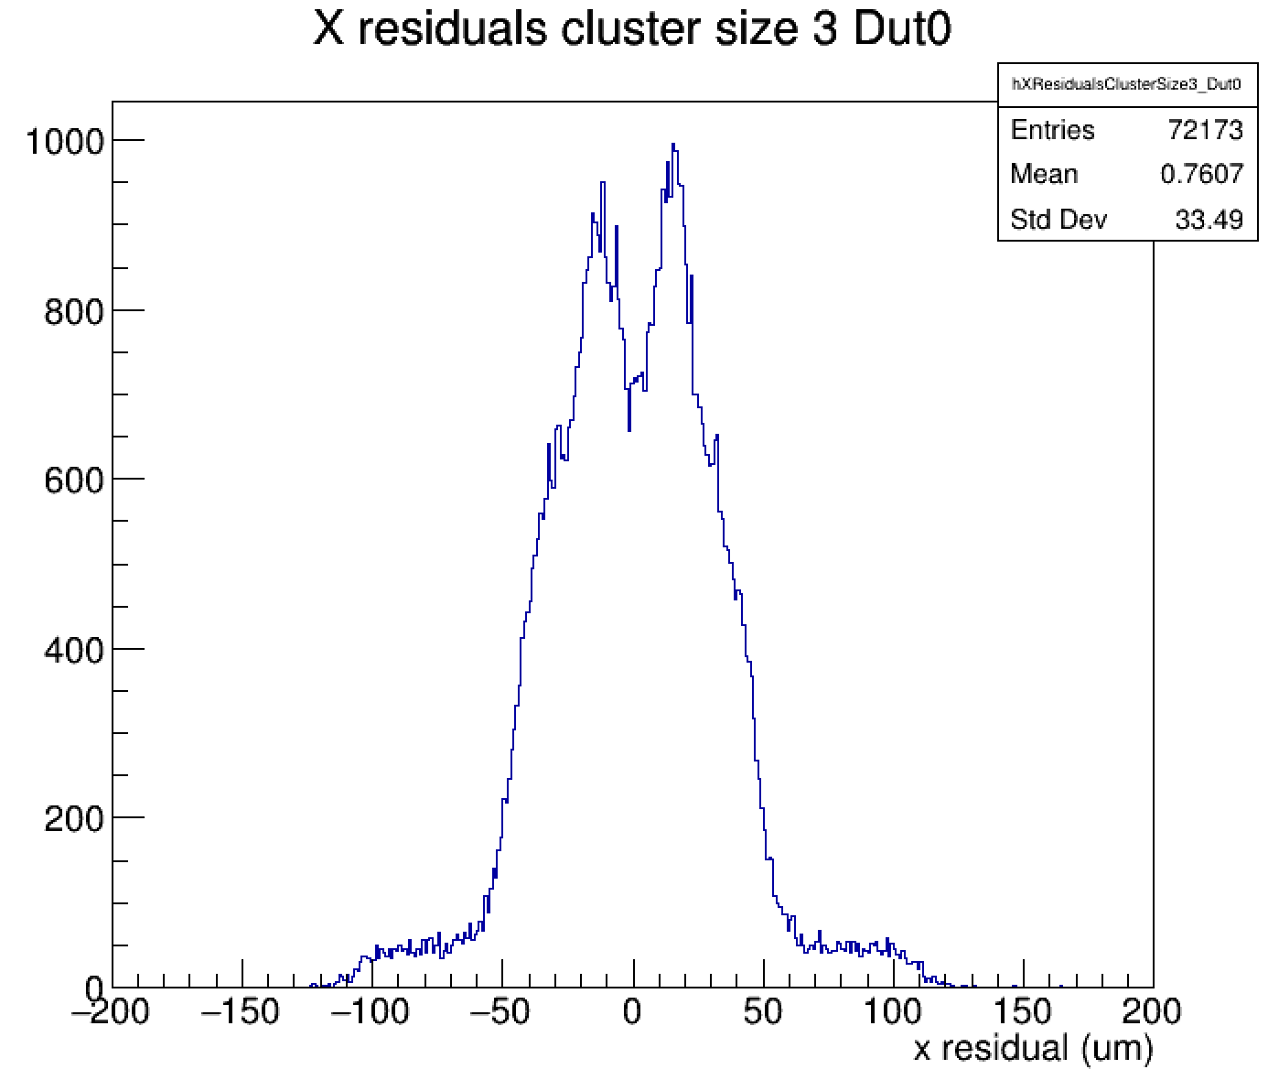
\includegraphics[width=\textwidth]{images/XRes_size3.png}
        \caption{}
        \label{fig:dist_b}
    \end{subfigure}

    \vspace{0.5cm}

    \begin{subfigure}[t]{0.5\textwidth}
        \centering
        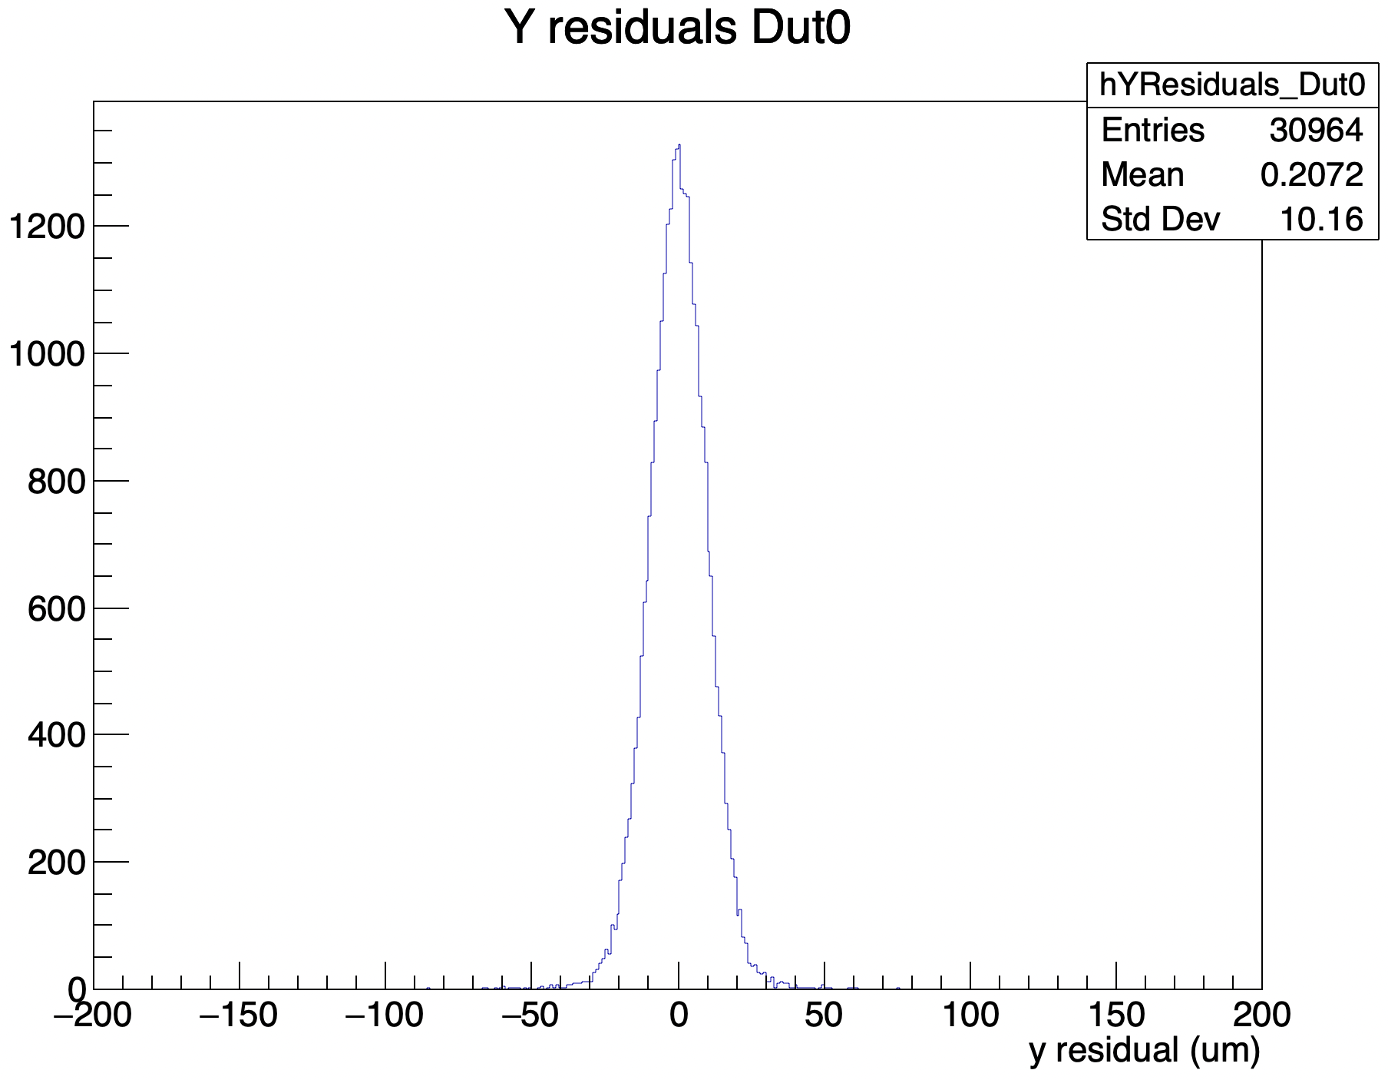
\includegraphics[width=\textwidth]{images/YRes_13planes.png}
        \caption{}
        \label{fig:dist_c}
    \end{subfigure}
    \hfill
    \begin{subfigure}[t]{0.45\textwidth}
        \centering
        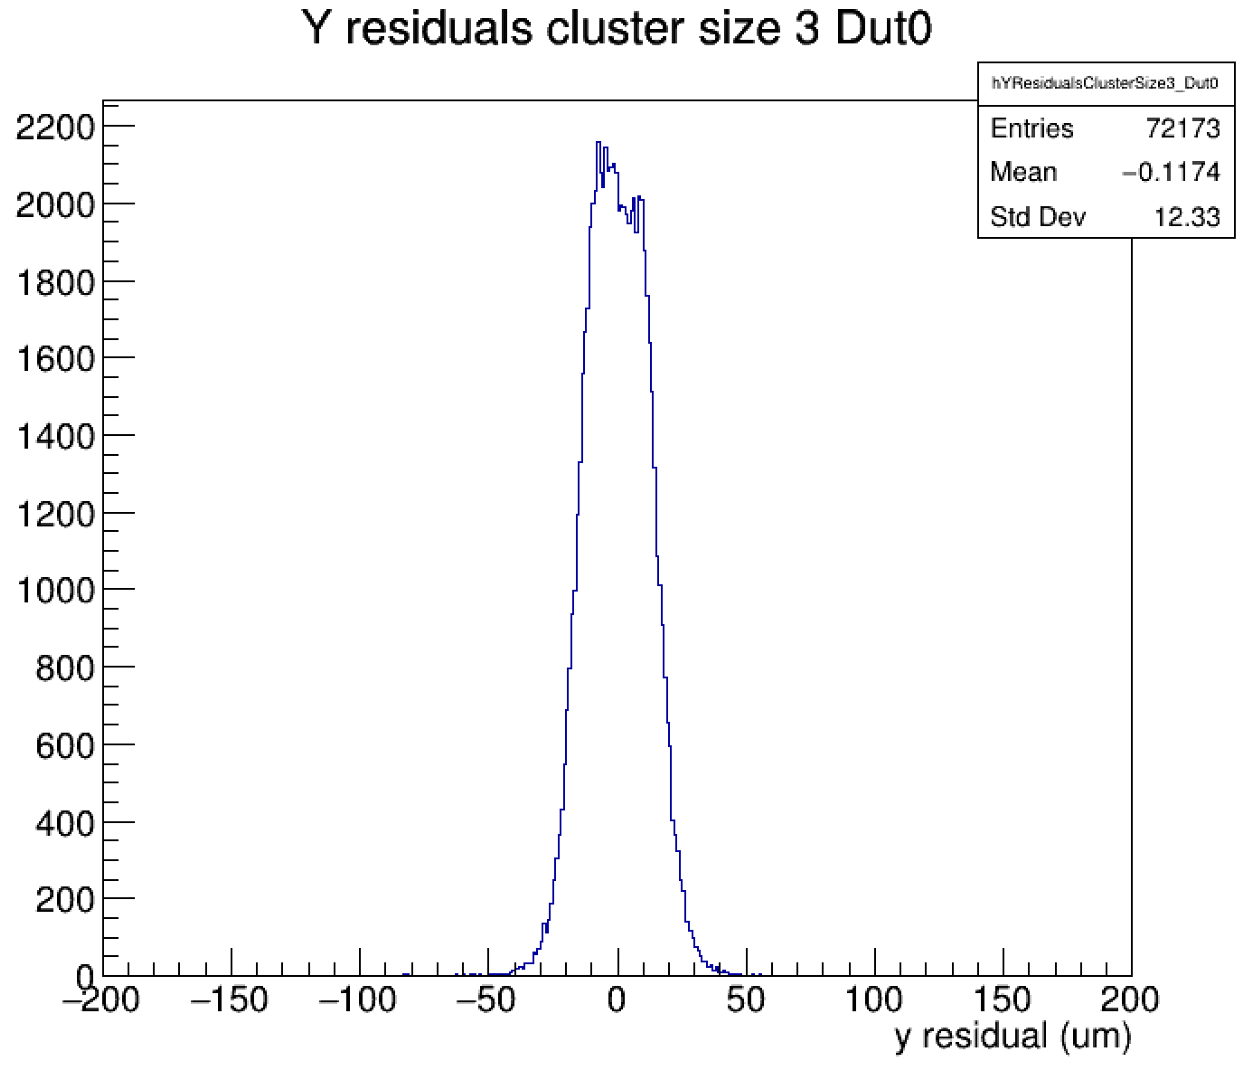
\includegraphics[width=\textwidth]{images/YRes_size3.png}
        \caption{}
        \label{fig:dist_d}
    \end{subfigure}

    \caption{Residual distributions in the X direction for cluster sizes 1 and 3 are shown in (a) and (b), respectively. Corresponding residuals in the Y direction for cluster sizes 1 and 3 are presented in (c) and (d).}
    \label{fig:resolution_size_1&3}
\end{figure}

In addition for the further investigation was important to look at the cluster size distribution for the different charge Bins. The results are shown in Figure~\ref{fig:cluster_bins_vs_size}. The results show that the cluster sizes increase as the charge Bin decreases. This supports the expectation, as delta-ray candidates (Bin 0) are anticipated to produce larger clusters than other charge Bins. Additionally, for the remaining charge Bins, the cluster sizes also increase consistently.

\begin{figure}[H]
    \centering
    \begin{subfigure}[t]{0.45\textwidth}
        \centering
        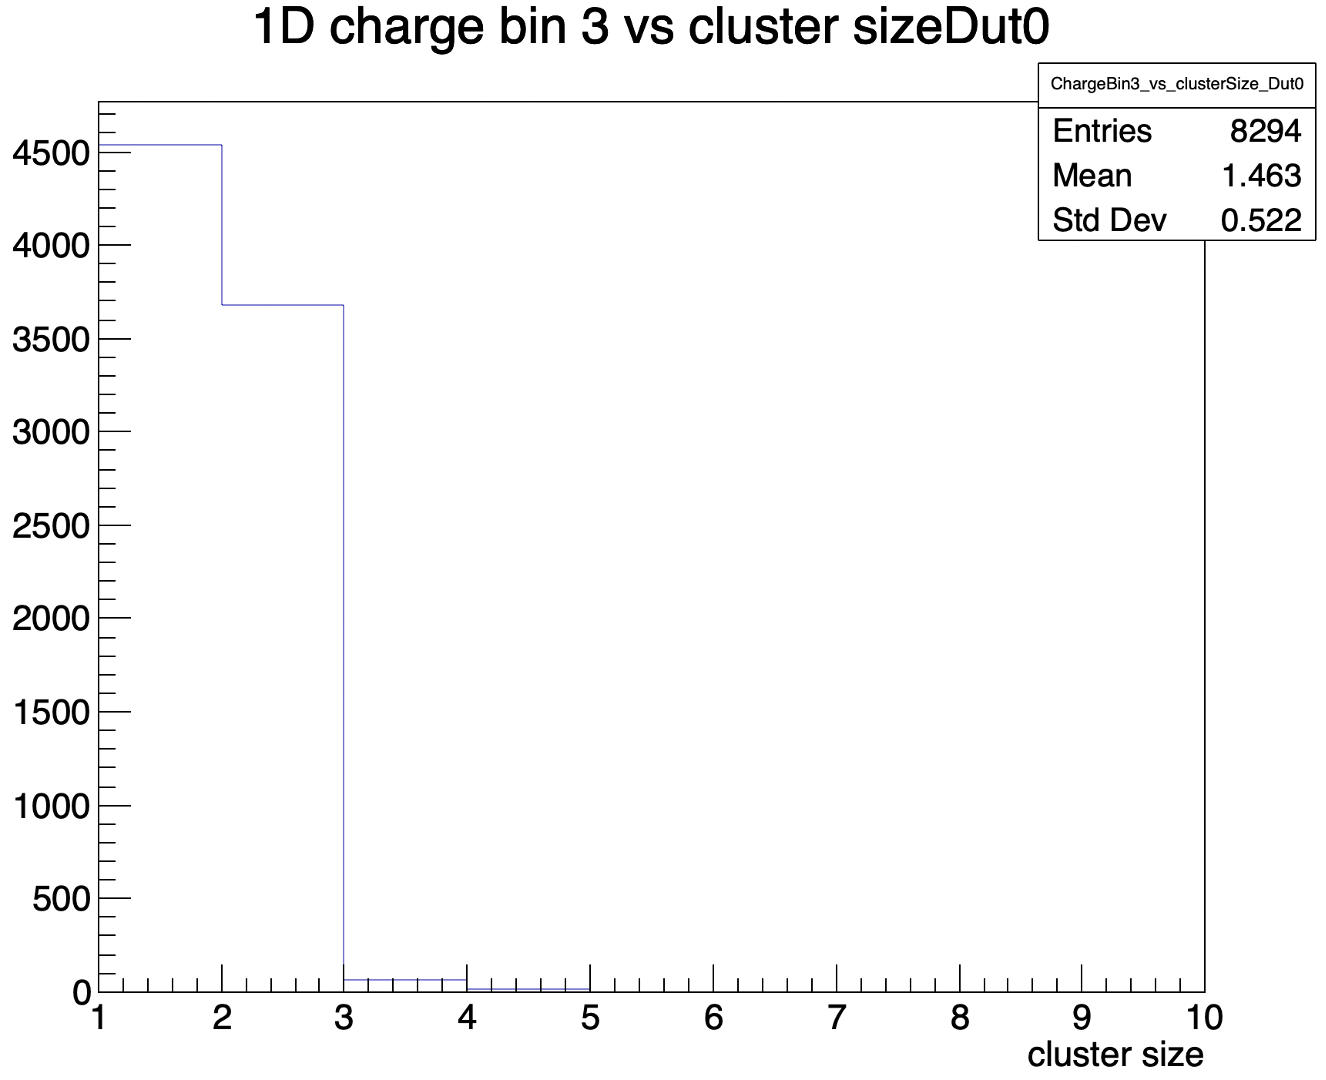
\includegraphics[width=\textwidth]{images/chargeBin3_us_clsize.png}
        \caption{}
        \label{fig:dist_a}
    \end{subfigure}
    \hfill
    \begin{subfigure}[t]{0.45\textwidth}
        \centering
        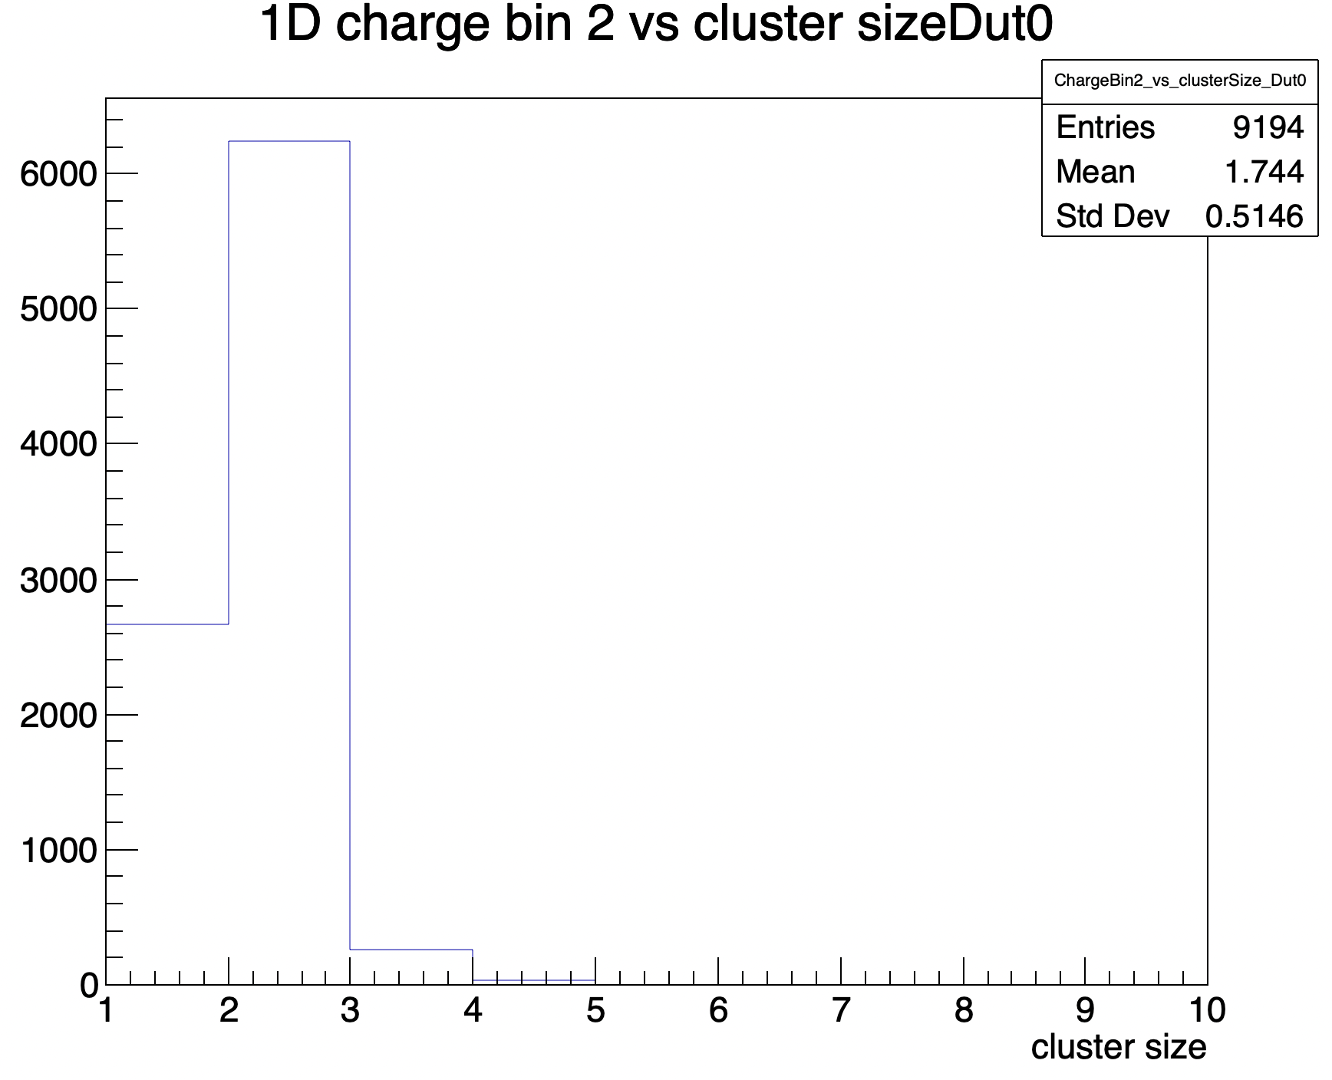
\includegraphics[width=\textwidth]{images/ClusBin2_us_clus_size.png}
        \caption{}
        \label{fig:dist_b}
    \end{subfigure}

    \vspace{0.5cm}

    \begin{subfigure}[t]{0.45\textwidth}
        \centering
        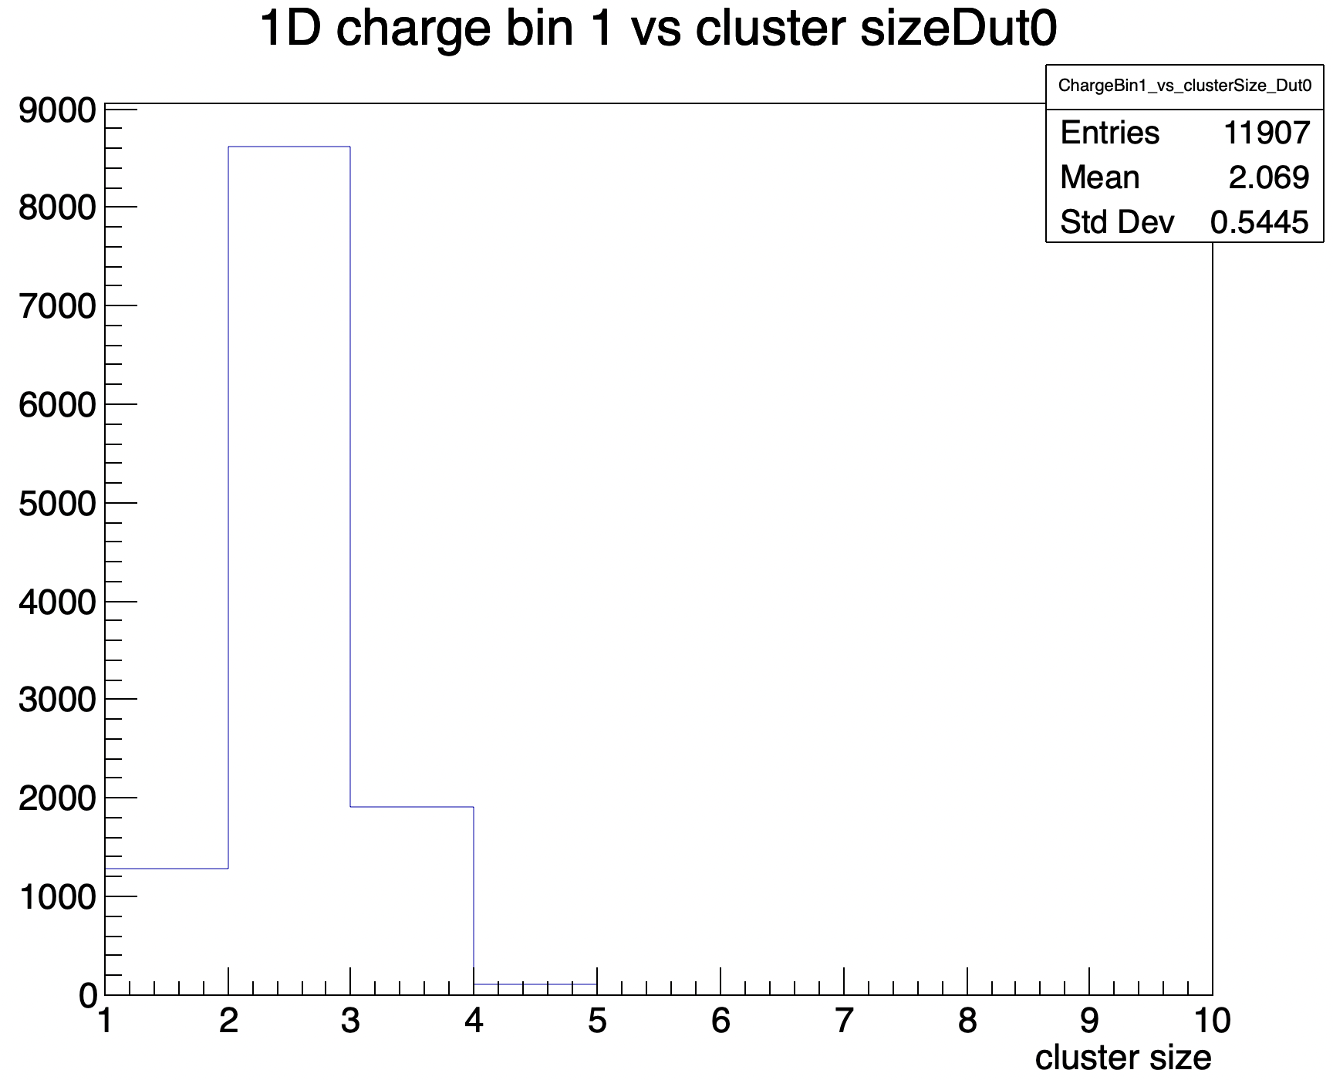
\includegraphics[width=\textwidth]{images/ChargeBin1_us_clus_size.png}
        \caption{}
        \label{fig:dist_c}
    \end{subfigure}
    \hfill
    \begin{subfigure}[t]{0.45\textwidth}
        \centering
        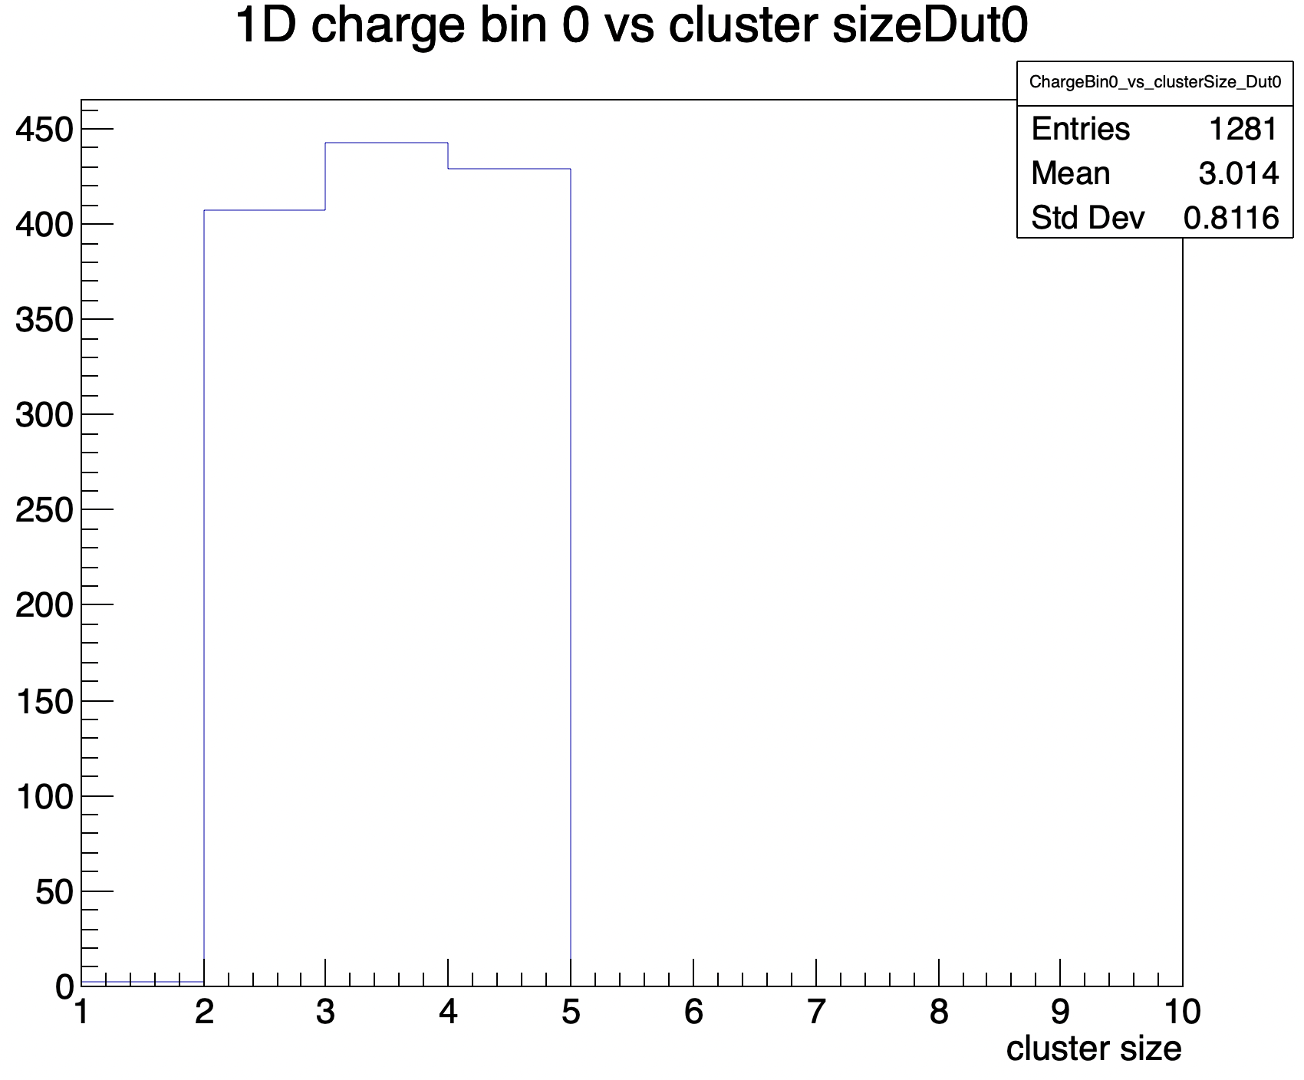
\includegraphics[width=\textwidth]{images/ChargeBin0_us_clus_size.png}
        \caption{}
        \label{fig:dist_d}
    \end{subfigure}

    \caption{Charge Bins versus cluster size of produced clusters for Bin~3 (a), Bin~2 (b), Bin~1 (c), and Bin~0 (d), respectively where the cluster size is defined as the number of pixels in a cluster.}
    \label{fig:cluster_bins_vs_size}
\end{figure}

In order to investigate whether the exclusion of charge Bin 0 improves the resolution, the X and Y predicted errors were examined. By default, the alignment previously required each track to pass through at least 13 out of 16 planes. Additional results were produced with the stricter condition that each individual track must pass through all four pixel planes. The track reconstruction was performed using hits from all pixel planes, and the predicted errors were evaluated at the DUT. All configurations were compared, and the results are shown in Figure~\ref{fig:X_Y_Predicted_Errors}. The measurement precision improved significantly when tracks were required to pass through all pixel planes. However, although the precision also improved after excluding Bin 0 tracks (delta-ray candidates), the difference was relatively minor.

\begin{figure}[H]
    \centering

    \begin{subfigure}[b]{0.3\textwidth}
        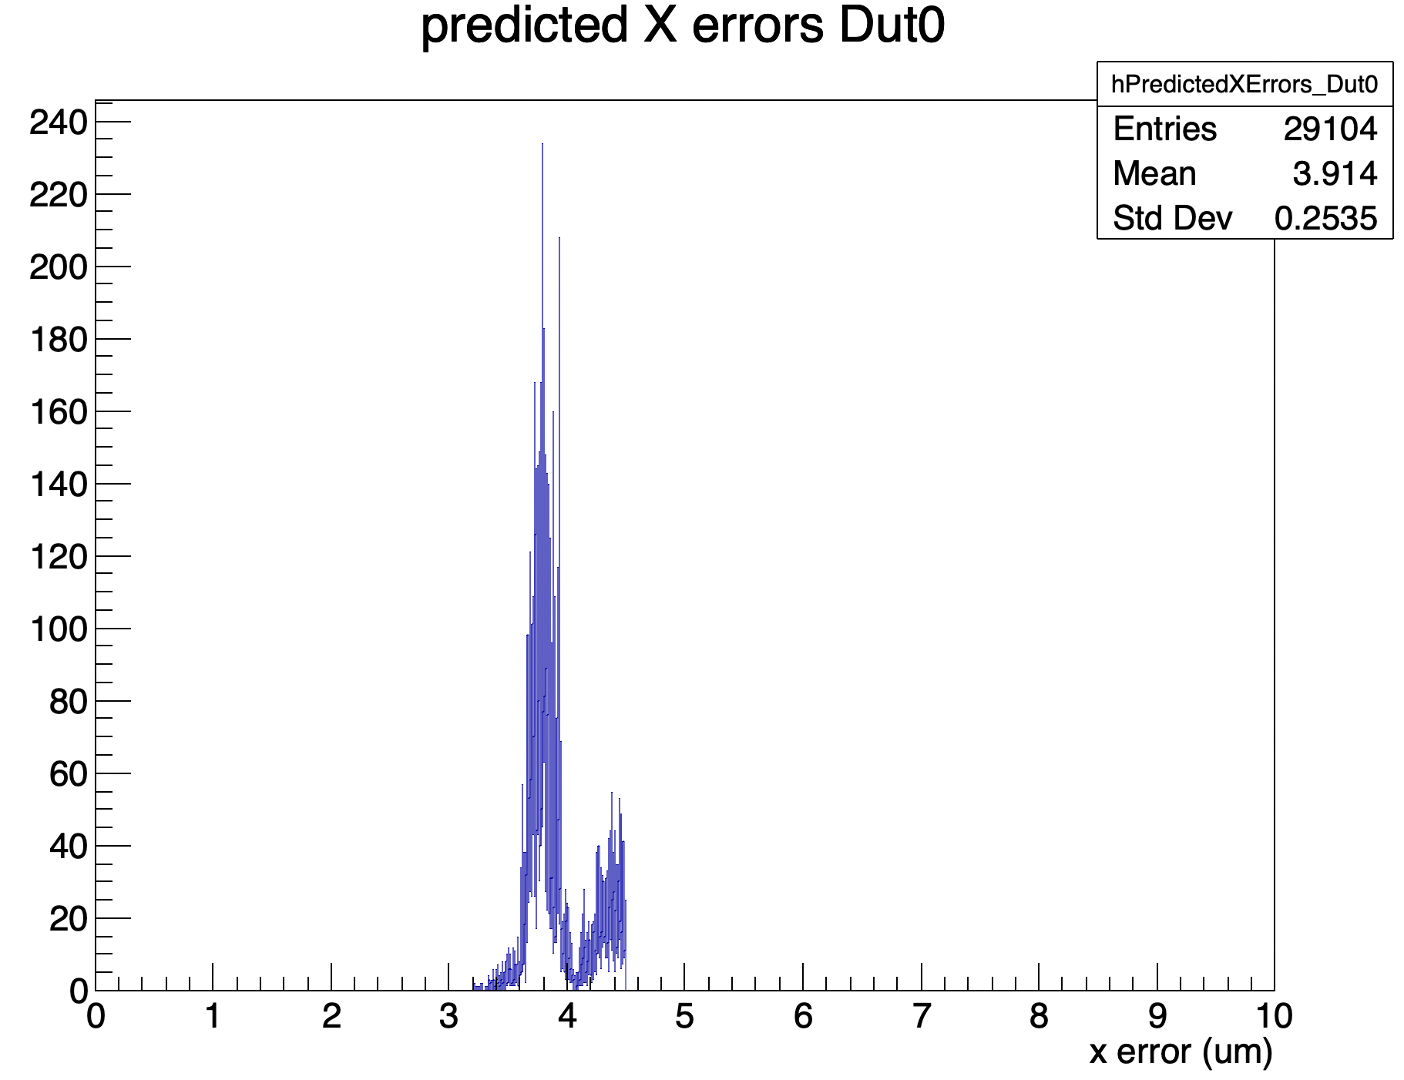
\includegraphics[width=\textwidth]{images/XPredError_13planes.png}
        \caption{}
    \end{subfigure}
    \hfill
    \begin{subfigure}[b]{0.33\textwidth}
        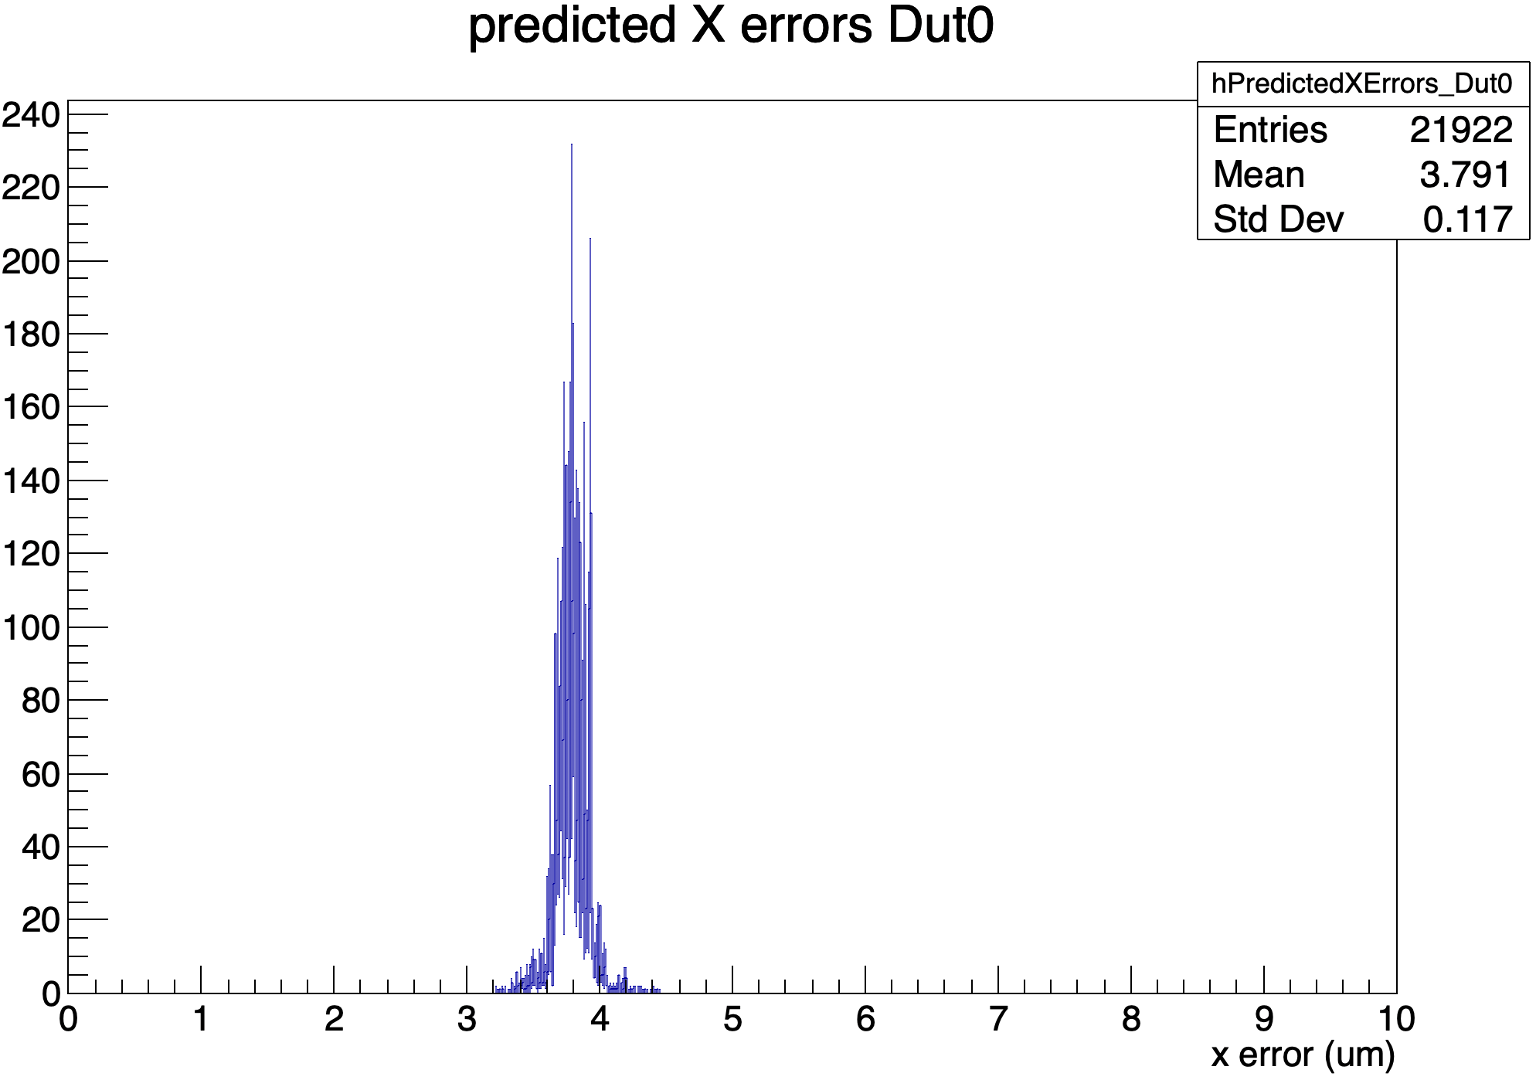
\includegraphics[width=\textwidth]{images/XPredError_4pixel.png}
        \caption{}
    \end{subfigure}
    \hfill
    \begin{subfigure}[b]{0.3\textwidth}
        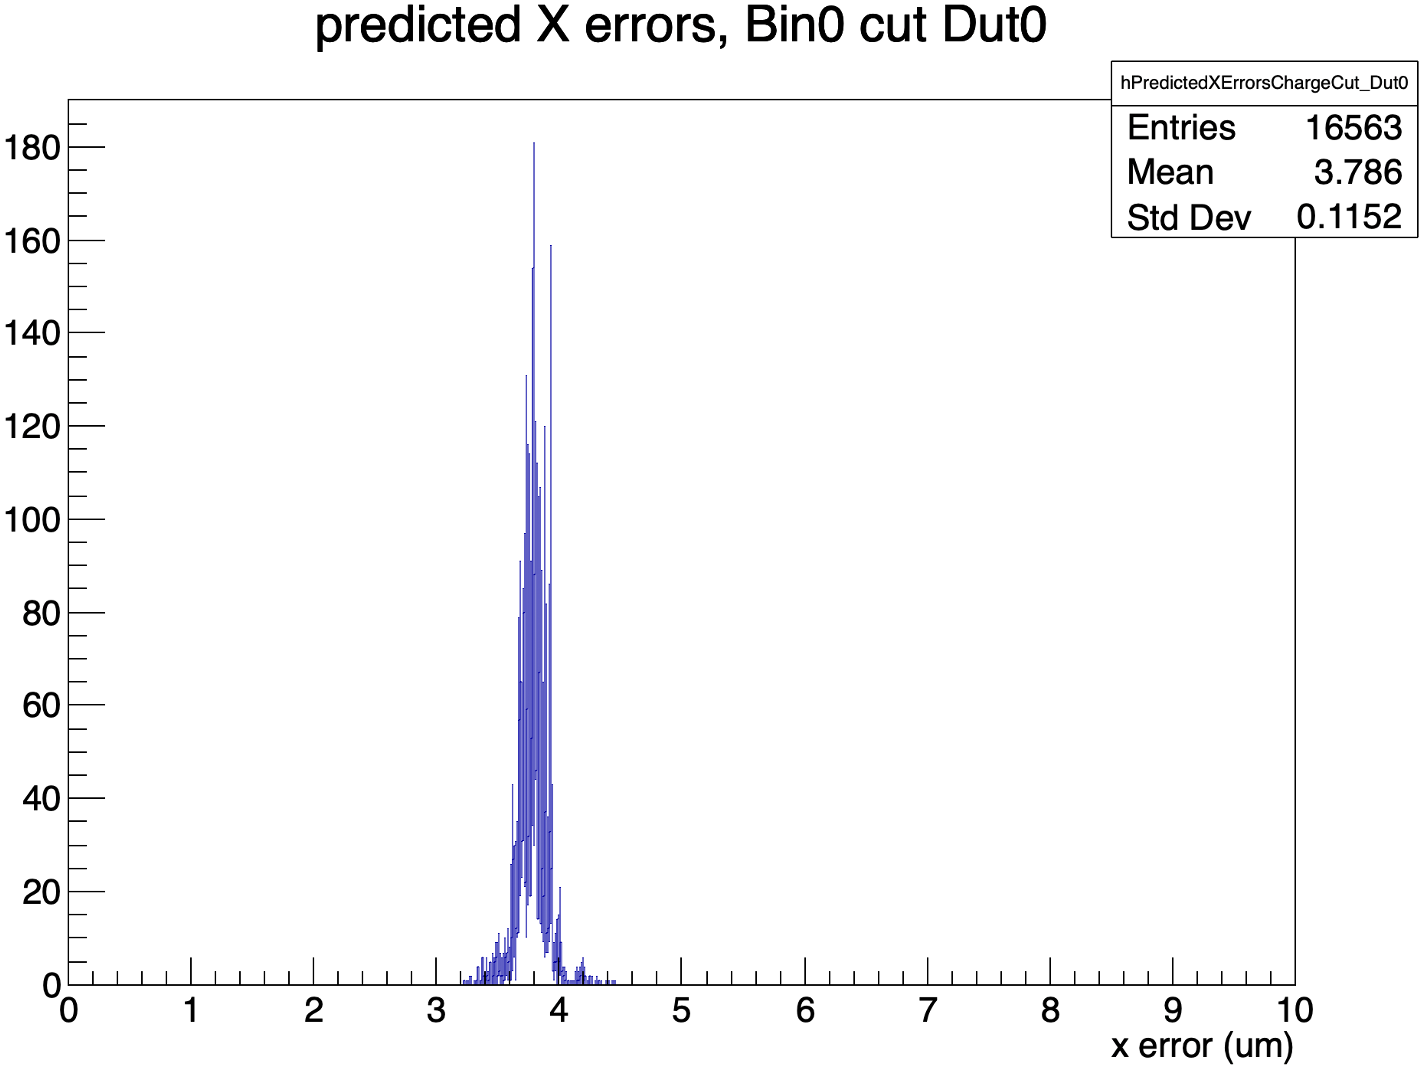
\includegraphics[width=\textwidth]{images/XPredError_4pixel_noBin0.png}
        \caption{}
    \end{subfigure}

    \vspace{0.5cm} % optional spacing between rows

    \begin{subfigure}[b]{0.3\textwidth}
        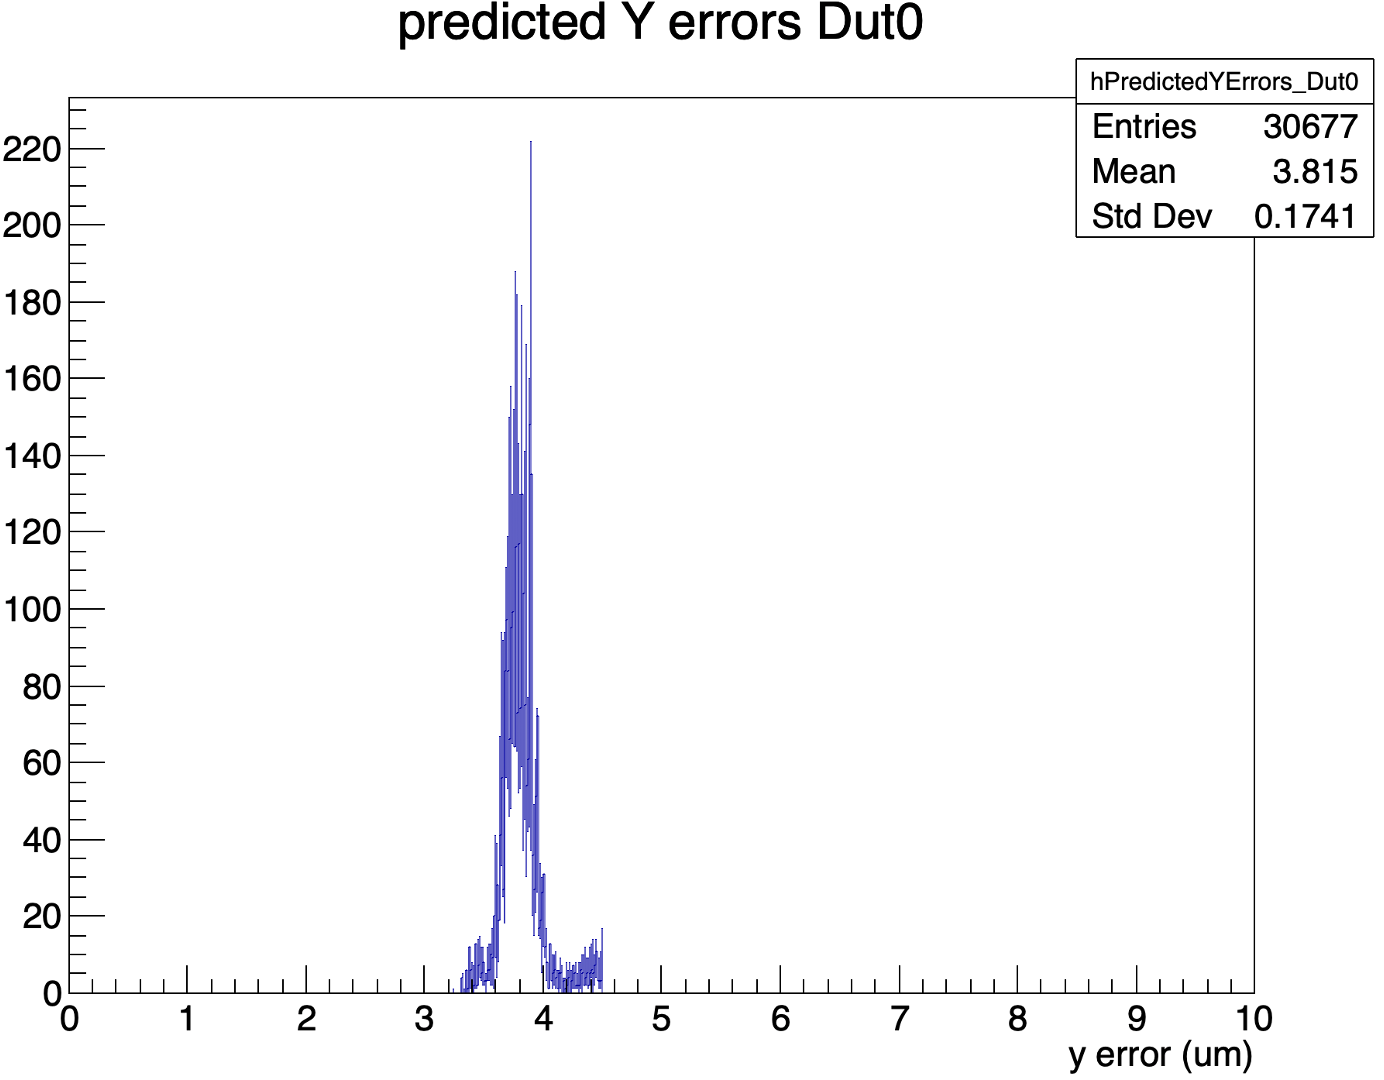
\includegraphics[width=\textwidth]{images/YPredicError_13planes.png}
        \caption{}
    \end{subfigure}
    \hfill
    \begin{subfigure}[b]{0.33\textwidth}
        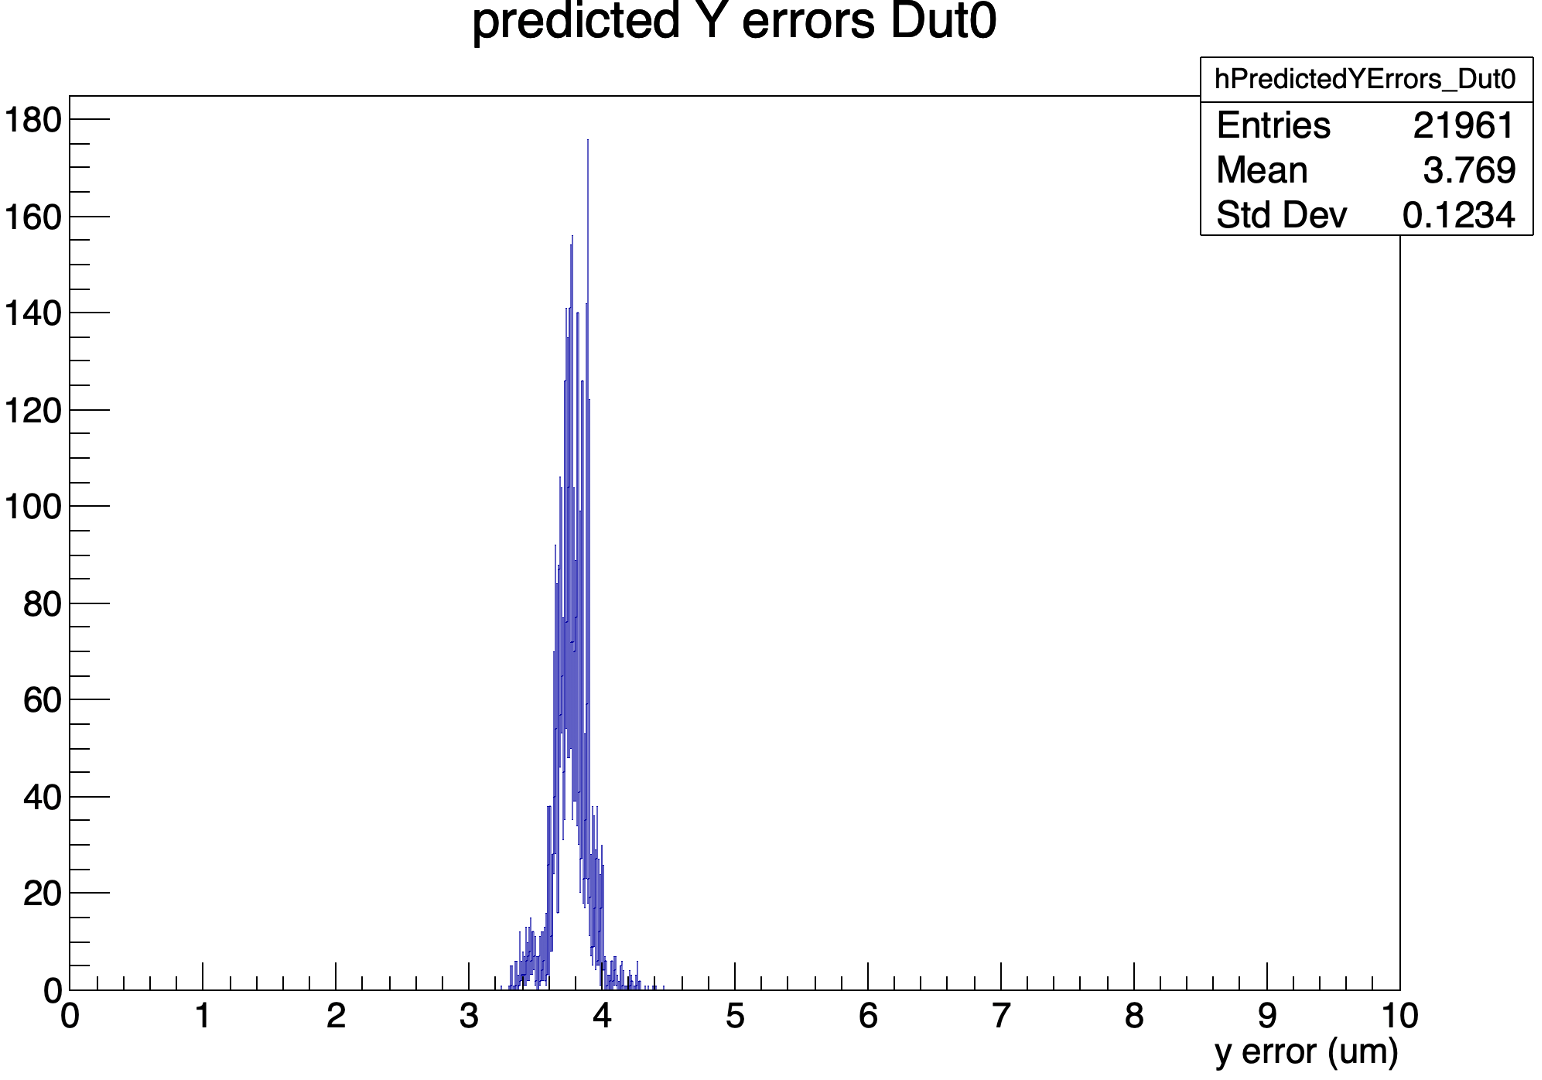
\includegraphics[width=\textwidth]{images/YPredError_4pixel.png}
        \caption{}
    \end{subfigure}
    \hfill
    \begin{subfigure}[b]{0.3\textwidth}
        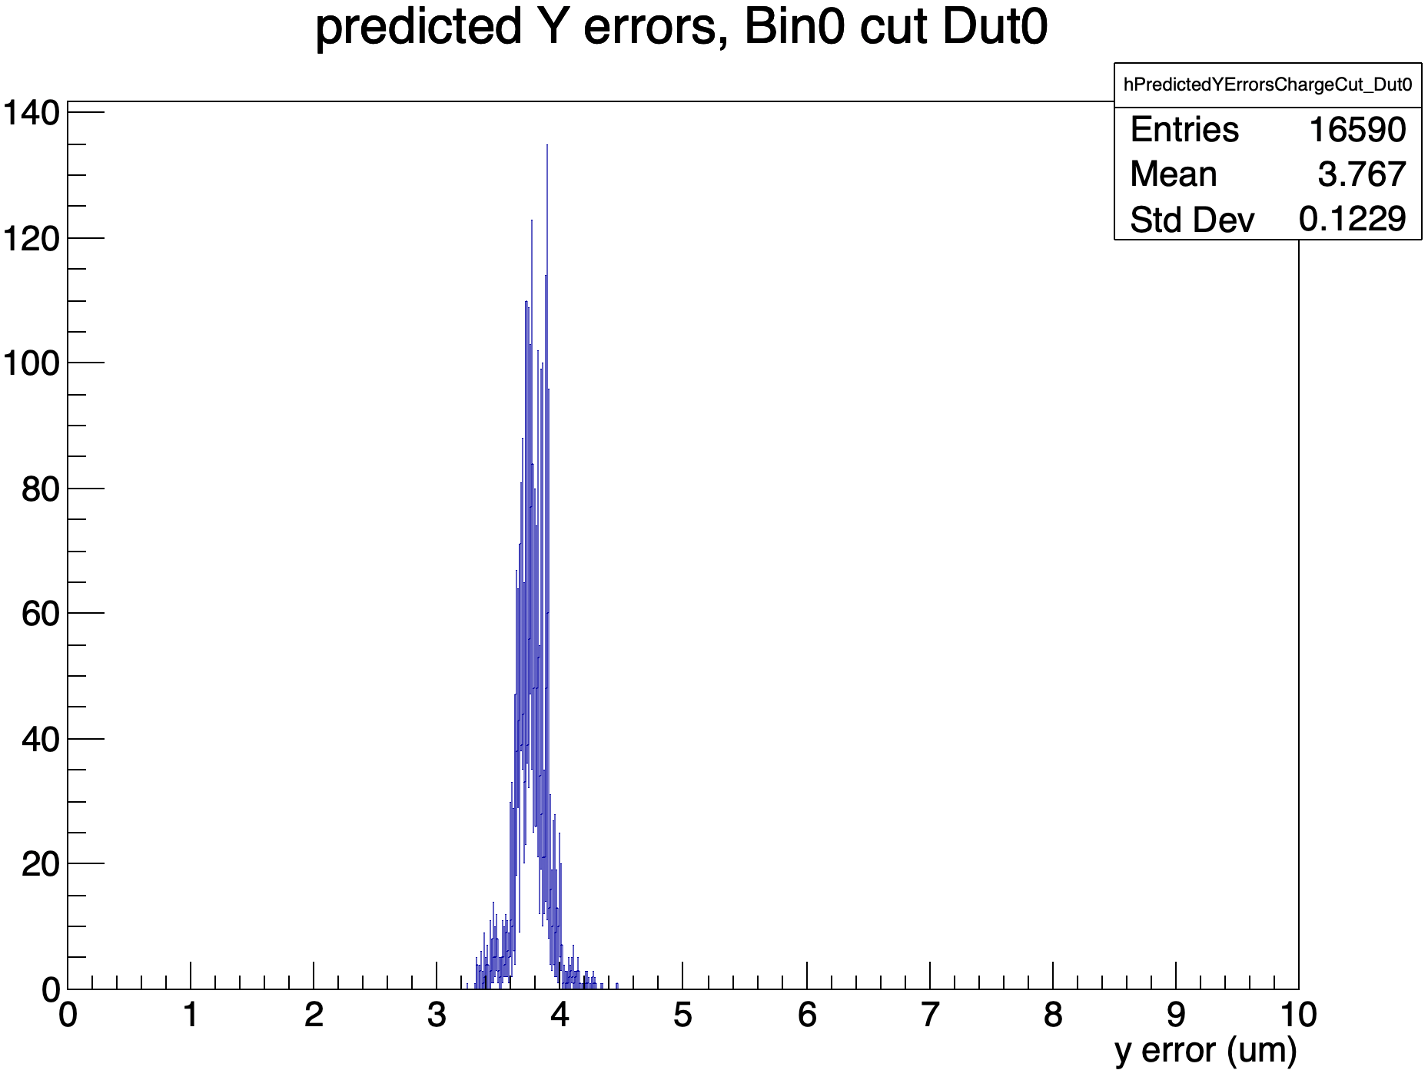
\includegraphics[width=\textwidth]{images/YPredError_4pixel_noBin0.png}
        \caption{}
    \end{subfigure}

    \caption{X predicted error for (a) for 13 planes (b) 4 pixel planes for certain (c) for 4 pixel planes with bin 0 cut and for (d-f) respective values but for Y predicted}
    \label{fig:X_Y_Predicted_Errors}
\end{figure}

Moreover, keeping the same conditions as for the predicted errors, the residuals were also examined. The results are shown in Figure~\ref{fig:X_Y_Residual_planes}. The residuals were calculated as the difference between the predicted and measured positions at the DUT. From the Y residual plots, we observe an improvement when applying the stricter requirement that all four pixel planes be used, as well as a performance enhancement when excluding Bin 0 tracks. However, applying the same restrictions in the X direction had the opposite effect. This requires some further investigation. A similar situation is observed in the residual plots for cluster size 1, shown in Figure~\ref{fig:X_Y_Residual_size_1_planes}.

\begin{figure}[H]
    \centering

    \begin{subfigure}[b]{0.3\textwidth}
        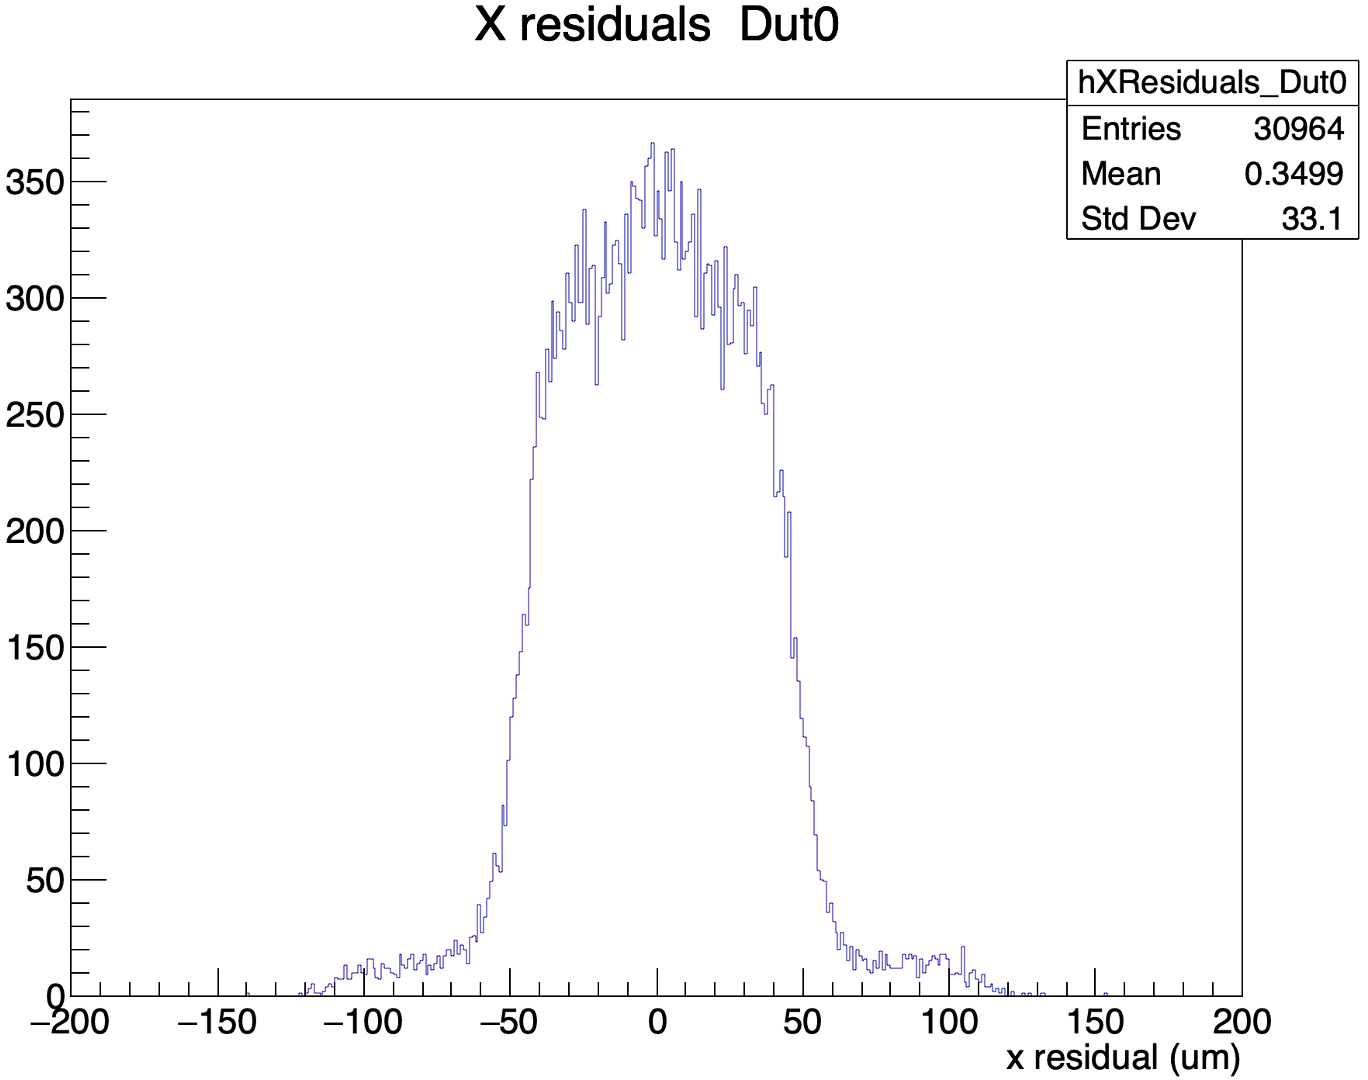
\includegraphics[width=\textwidth]{images/XRes_13planes.png}
        \caption{}
    \end{subfigure}
    \hfill
    \begin{subfigure}[b]{0.33\textwidth}
        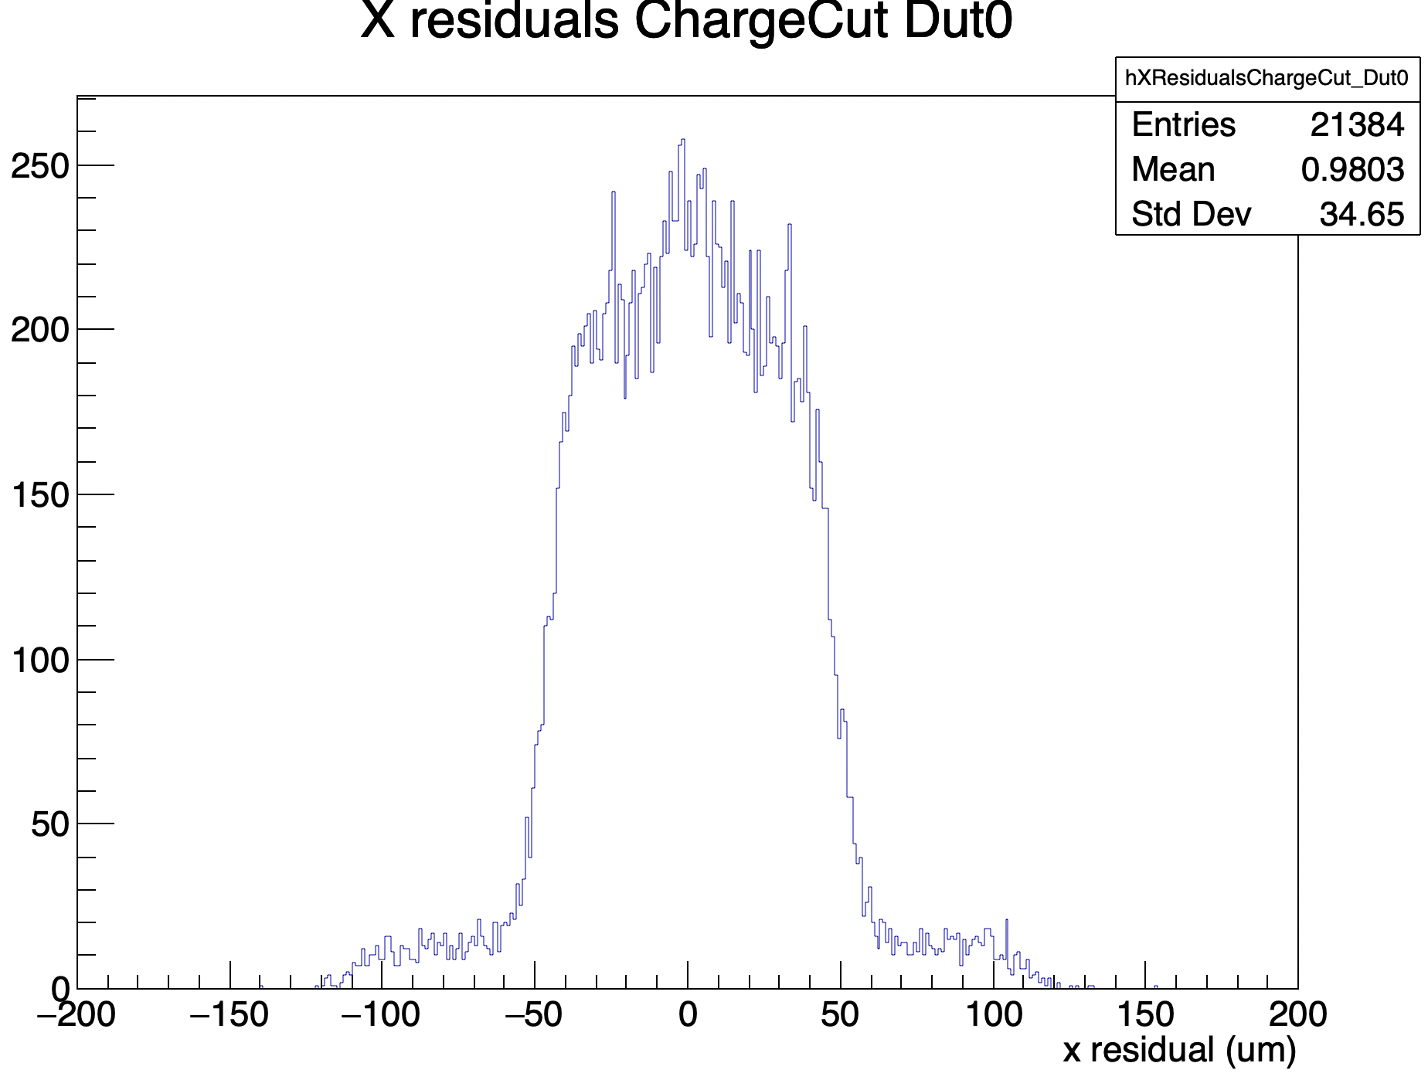
\includegraphics[width=\textwidth]{images/XRes_4pixel.png}
        \caption{}
    \end{subfigure}
    \hfill
    \begin{subfigure}[b]{0.3\textwidth}
        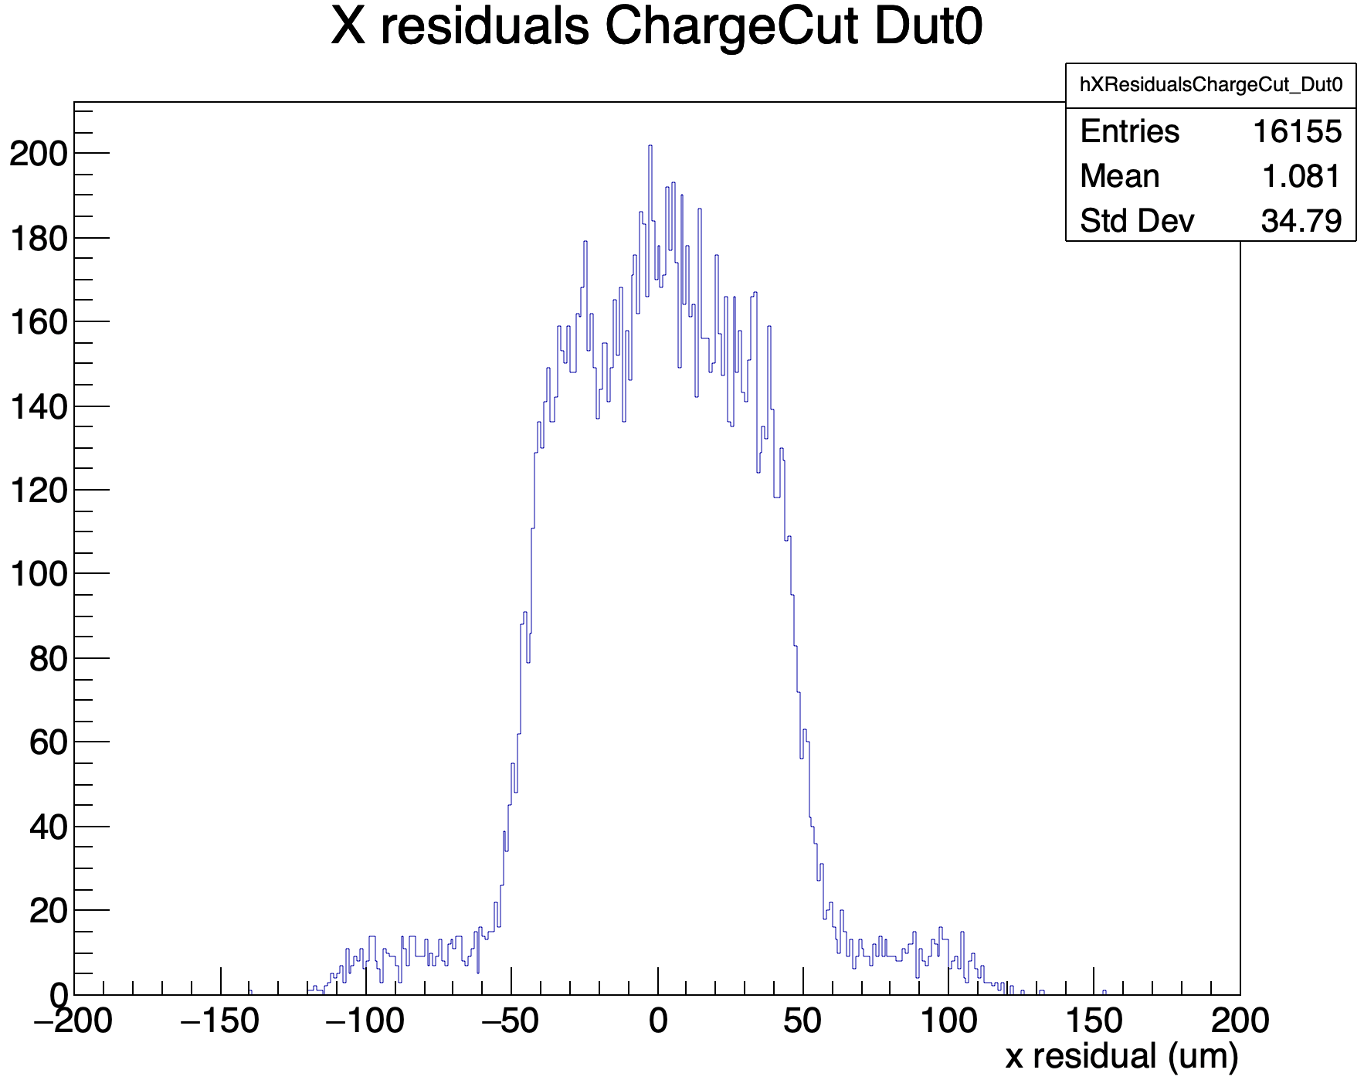
\includegraphics[width=\textwidth]{images/XRes_NoBin0_4pixel.png}
        \caption{}
    \end{subfigure}

    \vspace{0.5cm} % optional spacing between rows

    \begin{subfigure}[b]{0.3\textwidth}
        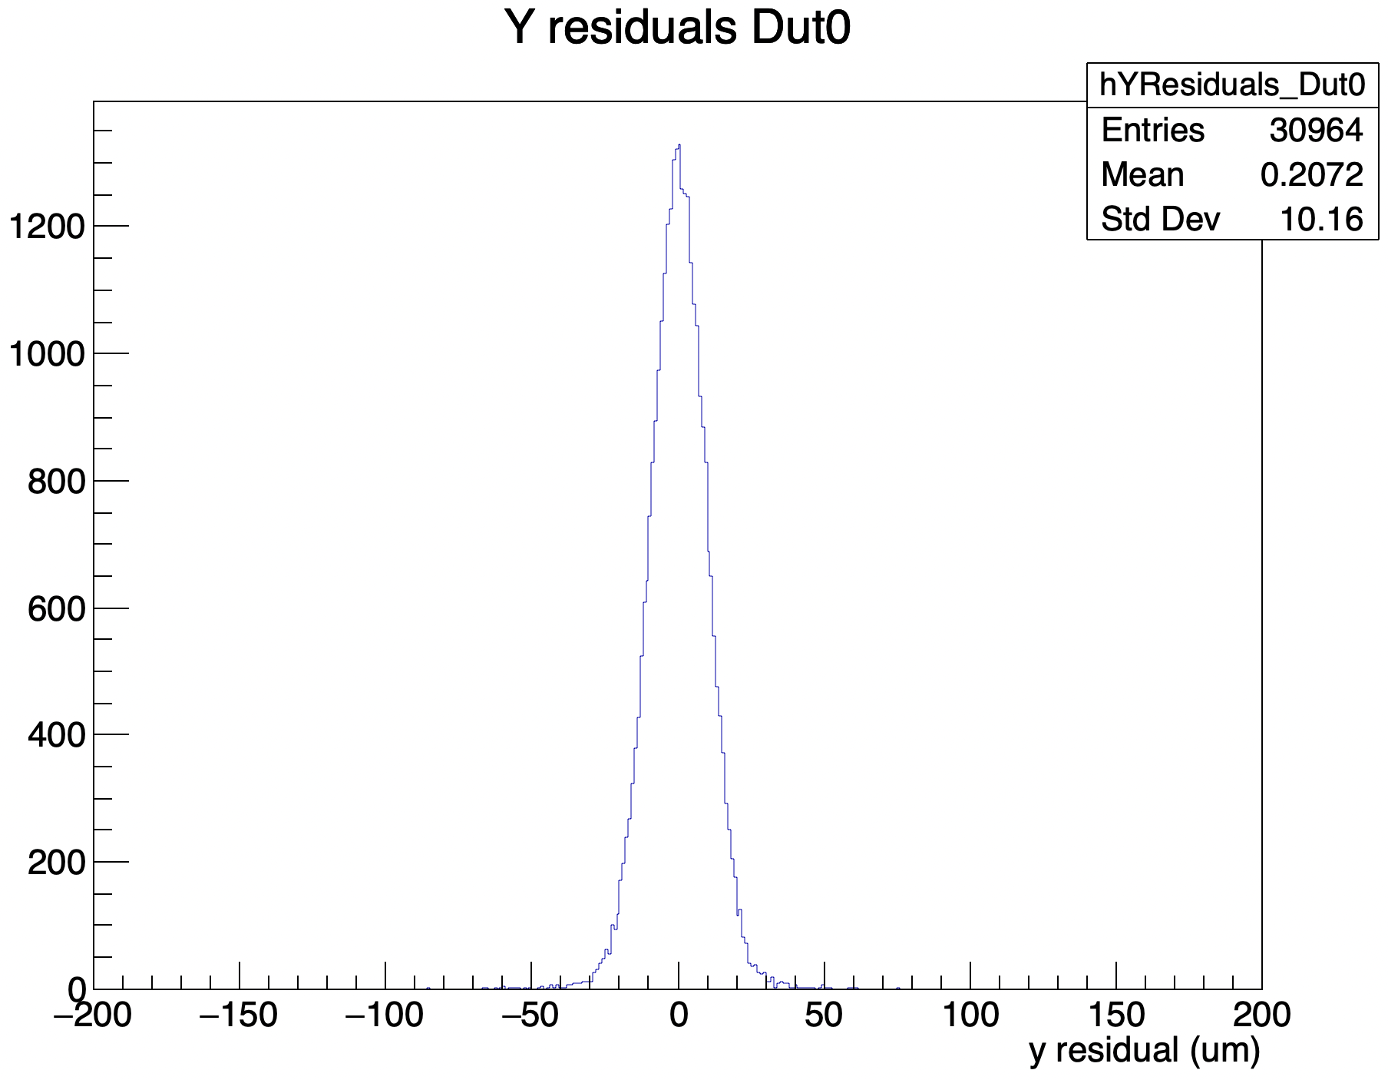
\includegraphics[width=\textwidth]{images/YRes_13planes.png}
        \caption{}
    \end{subfigure}
    \hfill
    \begin{subfigure}[b]{0.33\textwidth}
        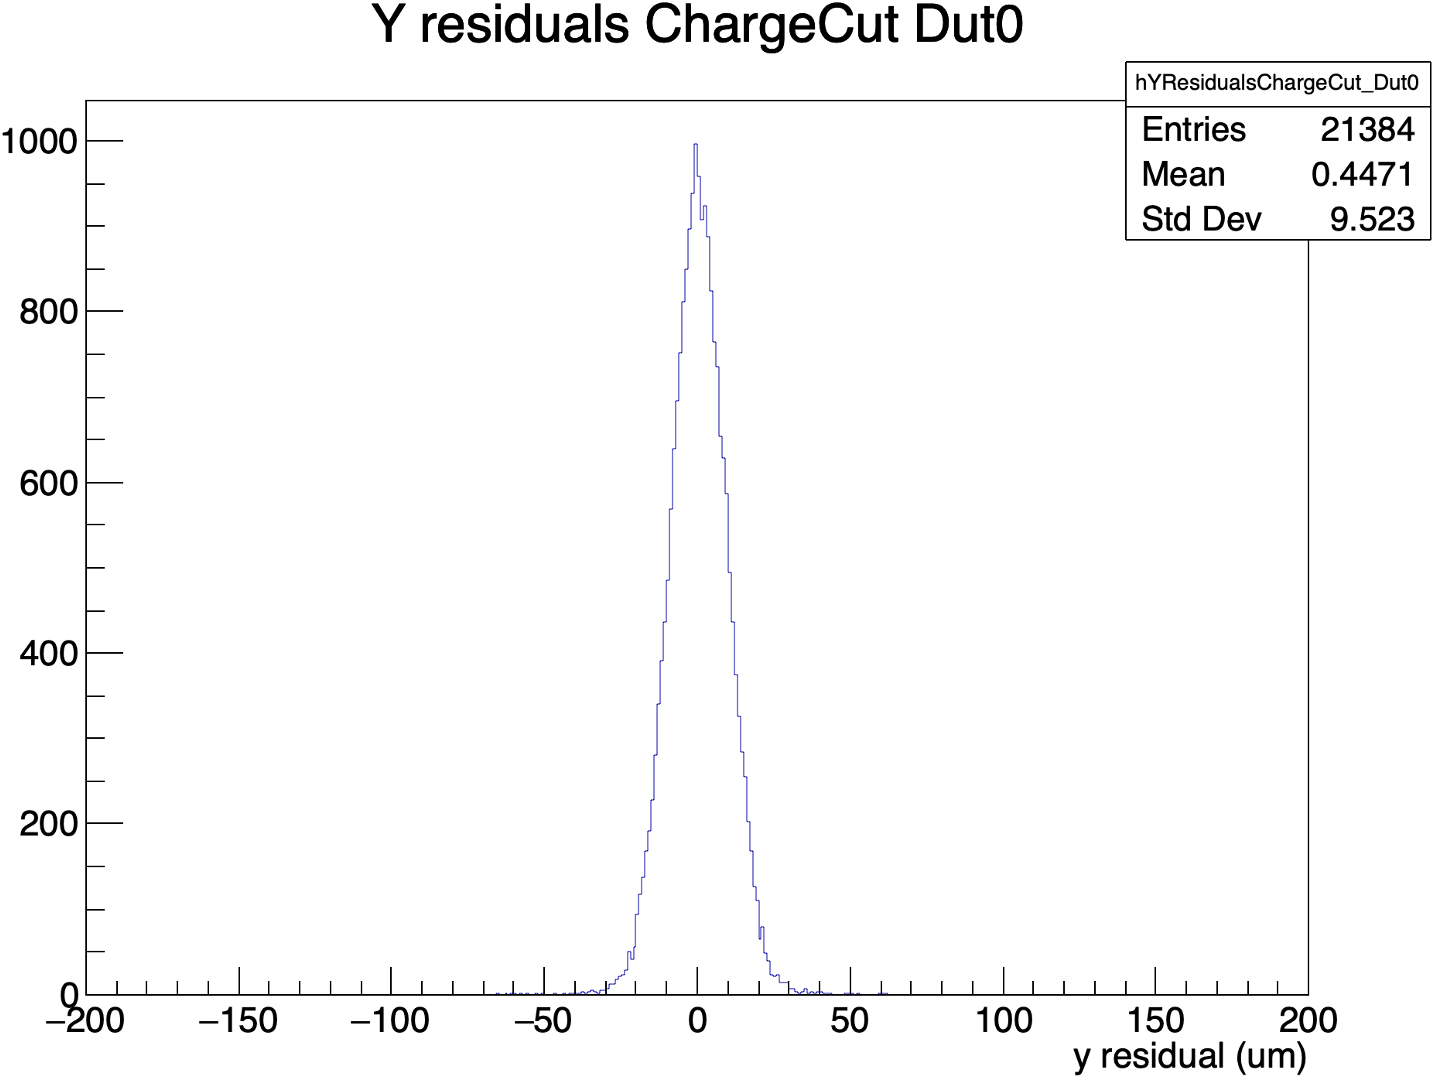
\includegraphics[width=\textwidth]{images/YRes_4pixel.png}
        \caption{}
    \end{subfigure}
    \hfill
    \begin{subfigure}[b]{0.3\textwidth}
        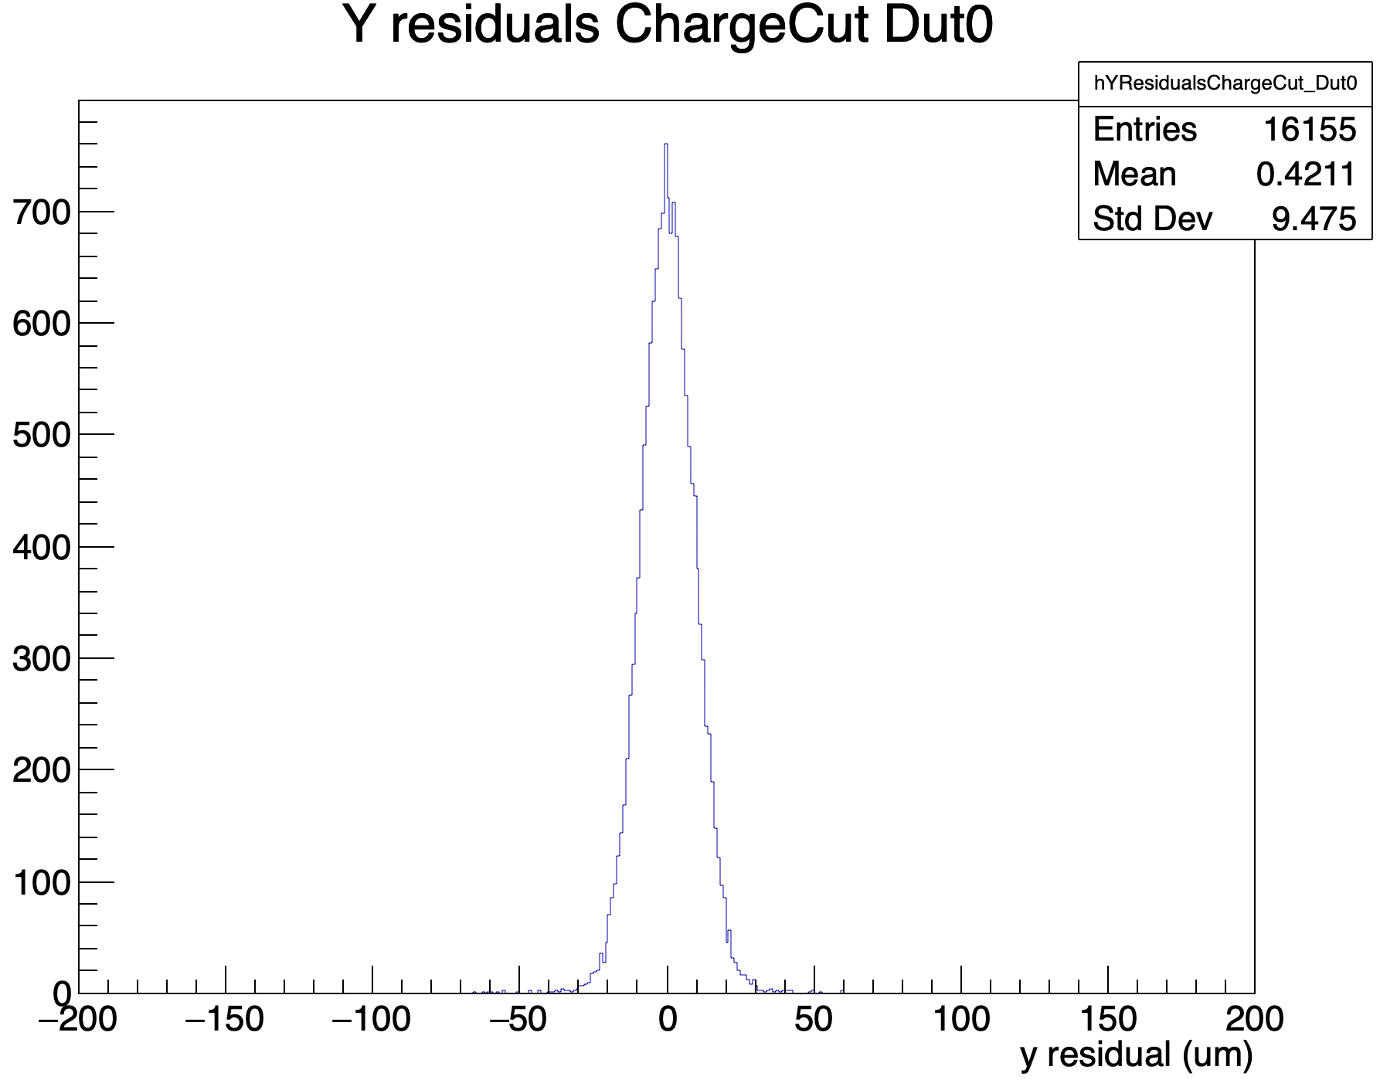
\includegraphics[width=\textwidth]{images/YRes_noBin0_4pixel.png}
        \caption{}
    \end{subfigure}

    \caption{X residuals are shown in panels (a--c): (a) for tracks passing through at least 13 planes, (b) for tracks passing through all 4 pixel planes, and (c) same as (b) but excluding Bin 0 (delta-ray) tracks. Panels (d--f) show the corresponding Y residuals under the same conditions.}
    \label{fig:X_Y_Residual_planes}
\end{figure}

In addition, asymmetry plots for different charge Bins were studied, with the expectation that the delta-ray charge Bin 0 would be more asymmetric than the others, indicating higher crosstalk. The charge asymmetry is defined as \( \frac{C_L - C_R}{C_L + C_R} \), where \( C_L \) and \( C_R \) are the charges collected by the cells to the left and right of the divide, respectively.
The results only for Right bump-bump are shown in Figure~\ref{fig:asymmetry_bins}.

\begin{figure}[H]
    \centering

    \begin{subfigure}[b]{0.3\textwidth}
        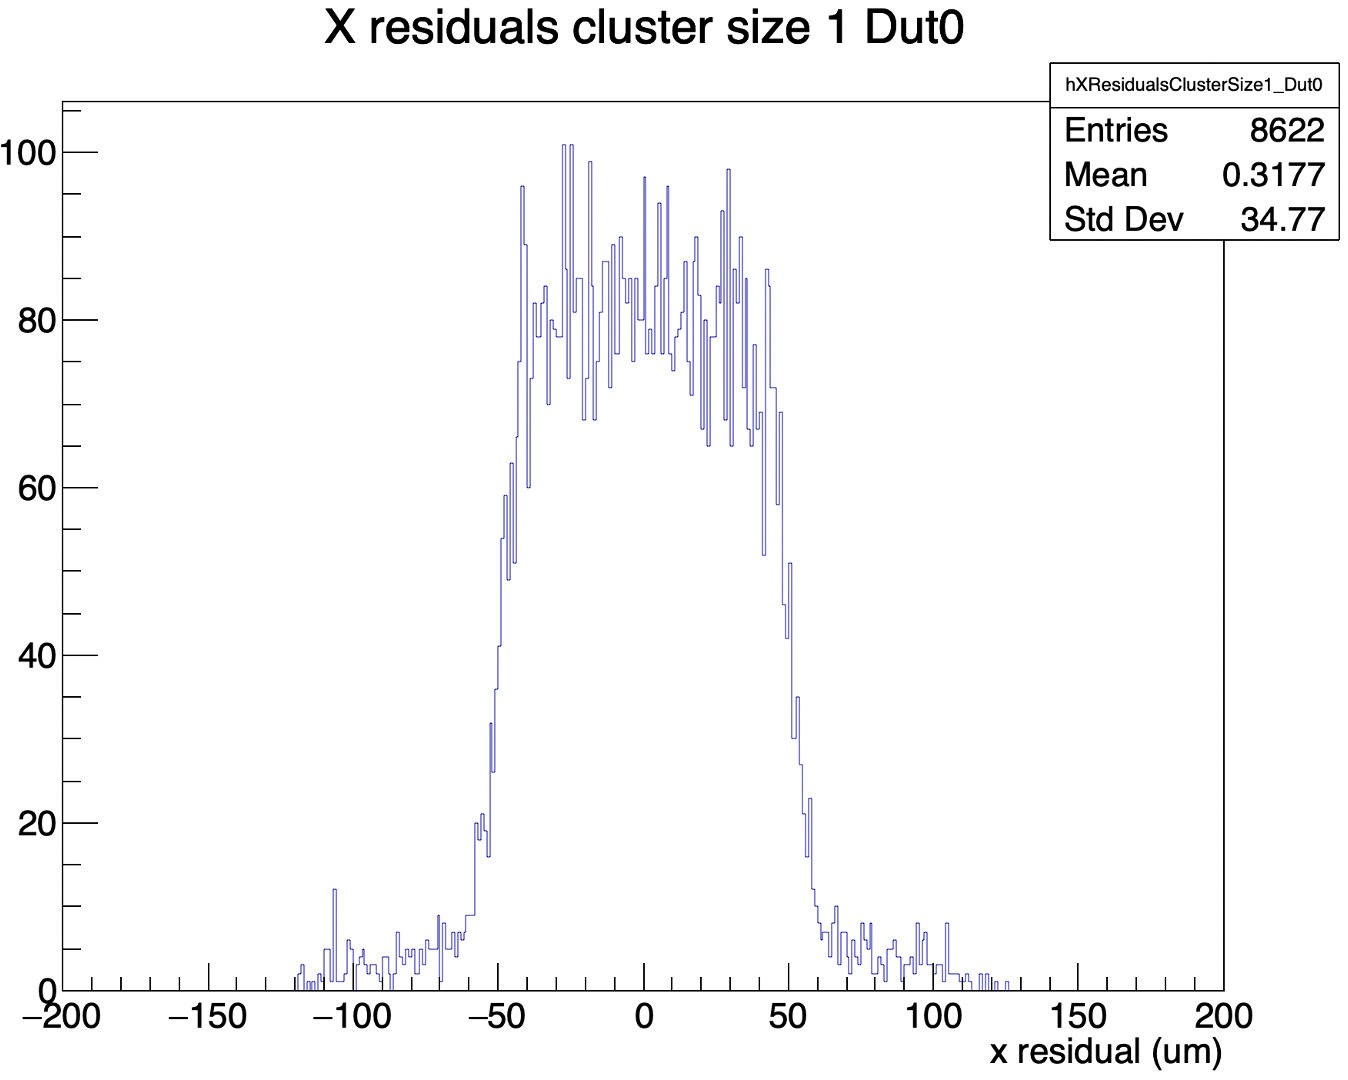
\includegraphics[width=\textwidth]{images/XRes_13plane_size1.png}
        \caption{}
    \end{subfigure}
    \hfill
    \begin{subfigure}[b]{0.33\textwidth}
        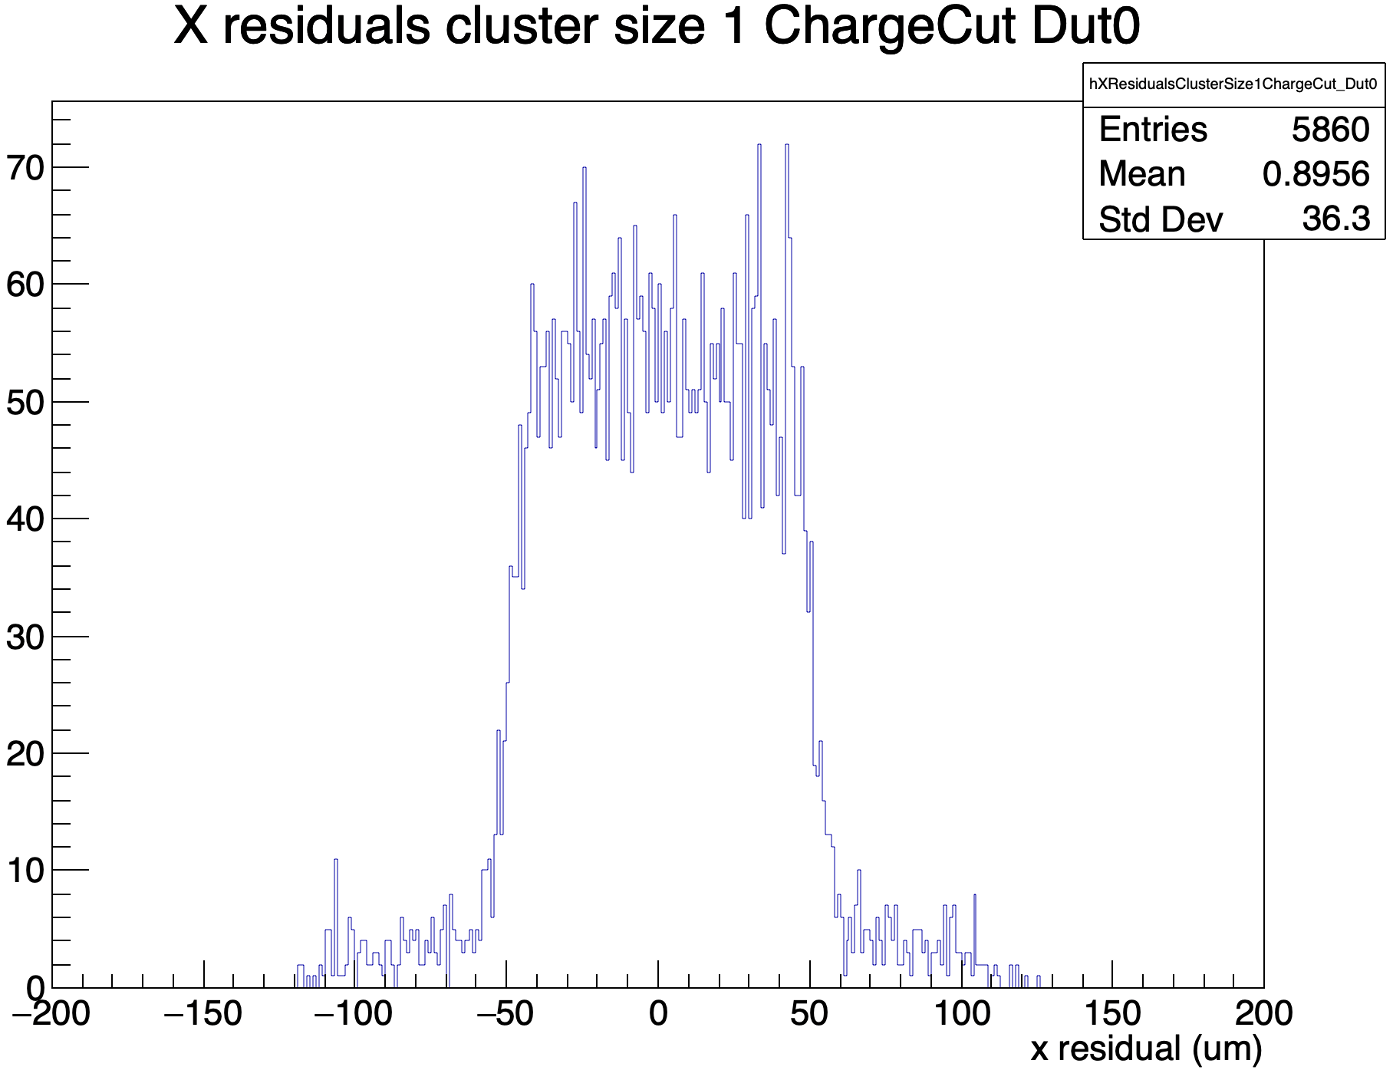
\includegraphics[width=\textwidth]{images/XRes_size1_4pixel.png}
        \caption{}
    \end{subfigure}
    \hfill
    \begin{subfigure}[b]{0.3\textwidth}
        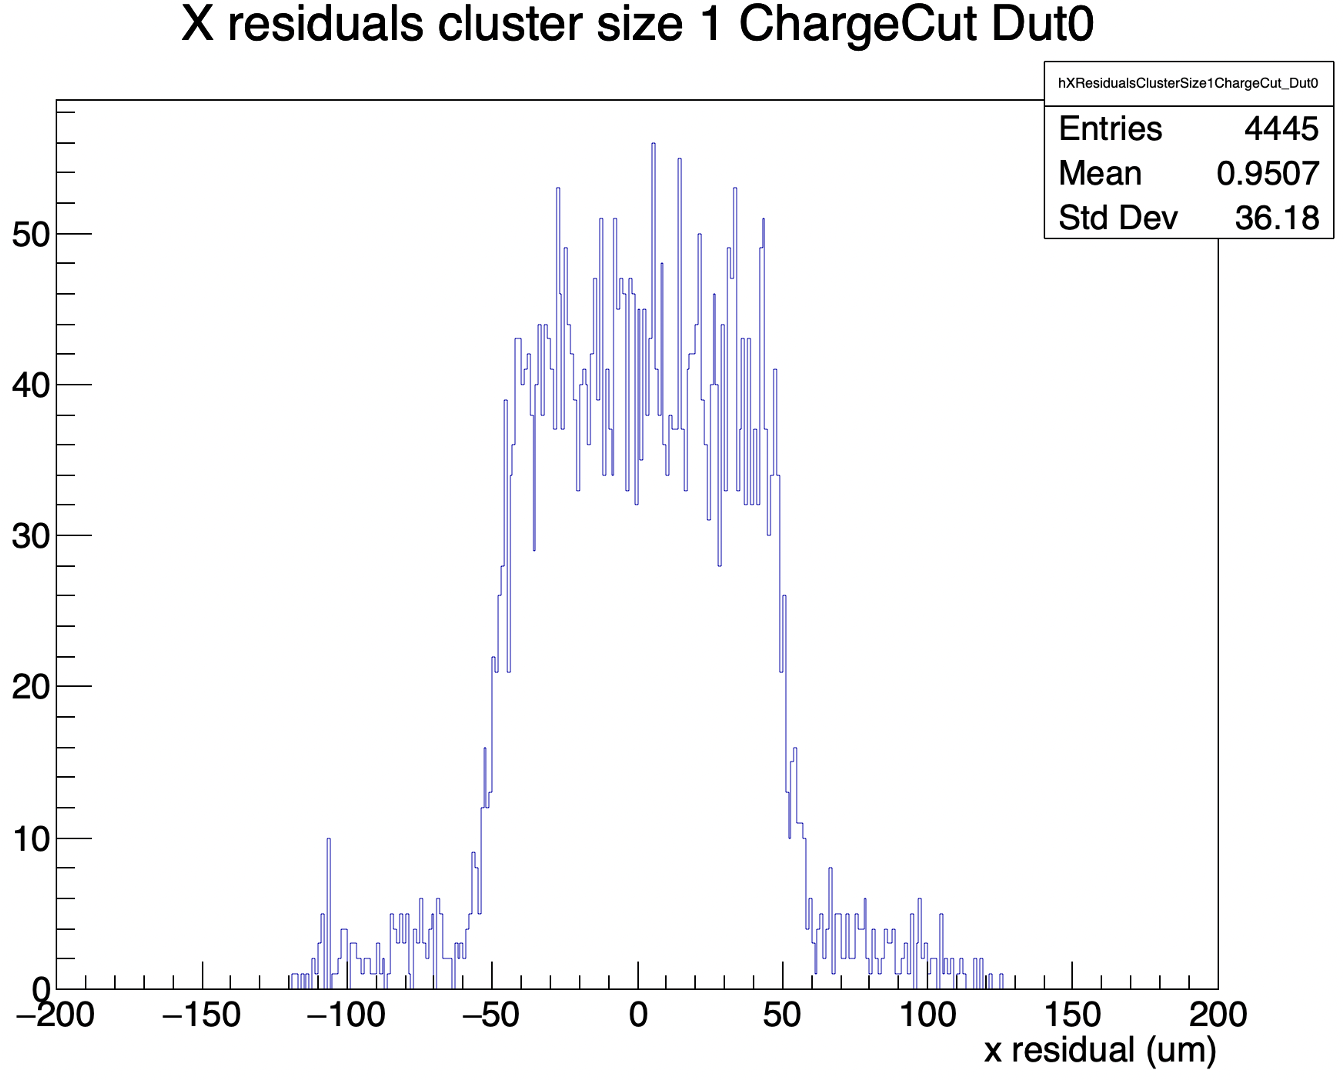
\includegraphics[width=\textwidth]{images/XRes_4pixel_noBin0_size1.png}
        \caption{}
    \end{subfigure}

    \vspace{0.5cm} % optional spacing between rows

    \begin{subfigure}[b]{0.3\textwidth}
        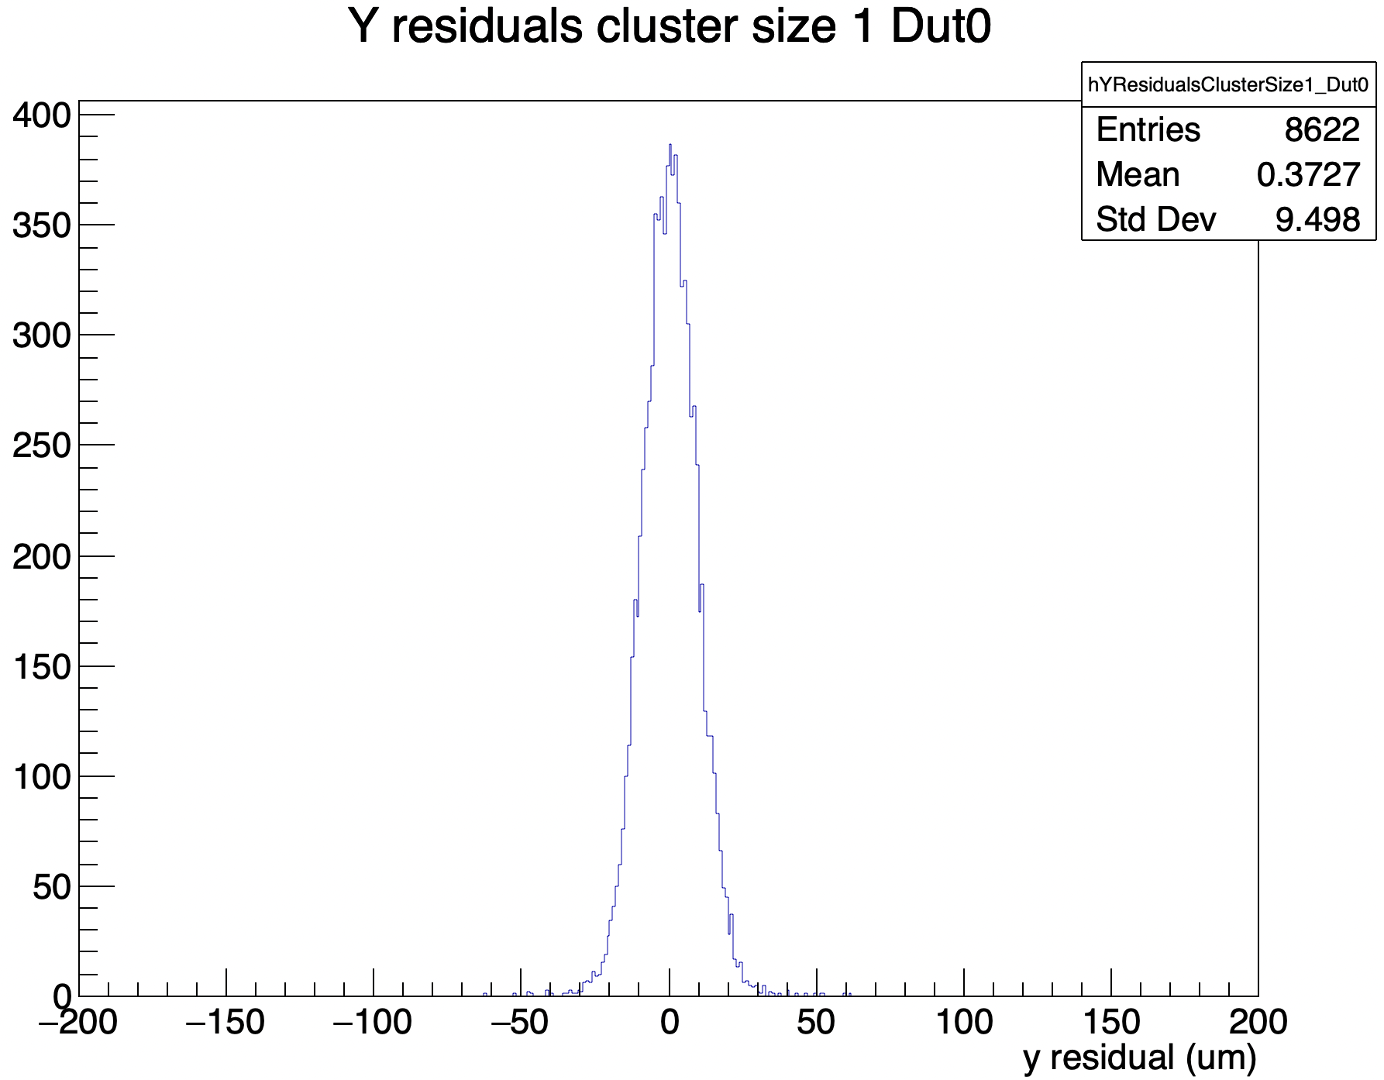
\includegraphics[width=\textwidth]{images/YRes_size1_13planes.png}
        \caption{}
    \end{subfigure}
    \hfill
    \begin{subfigure}[b]{0.33\textwidth}
        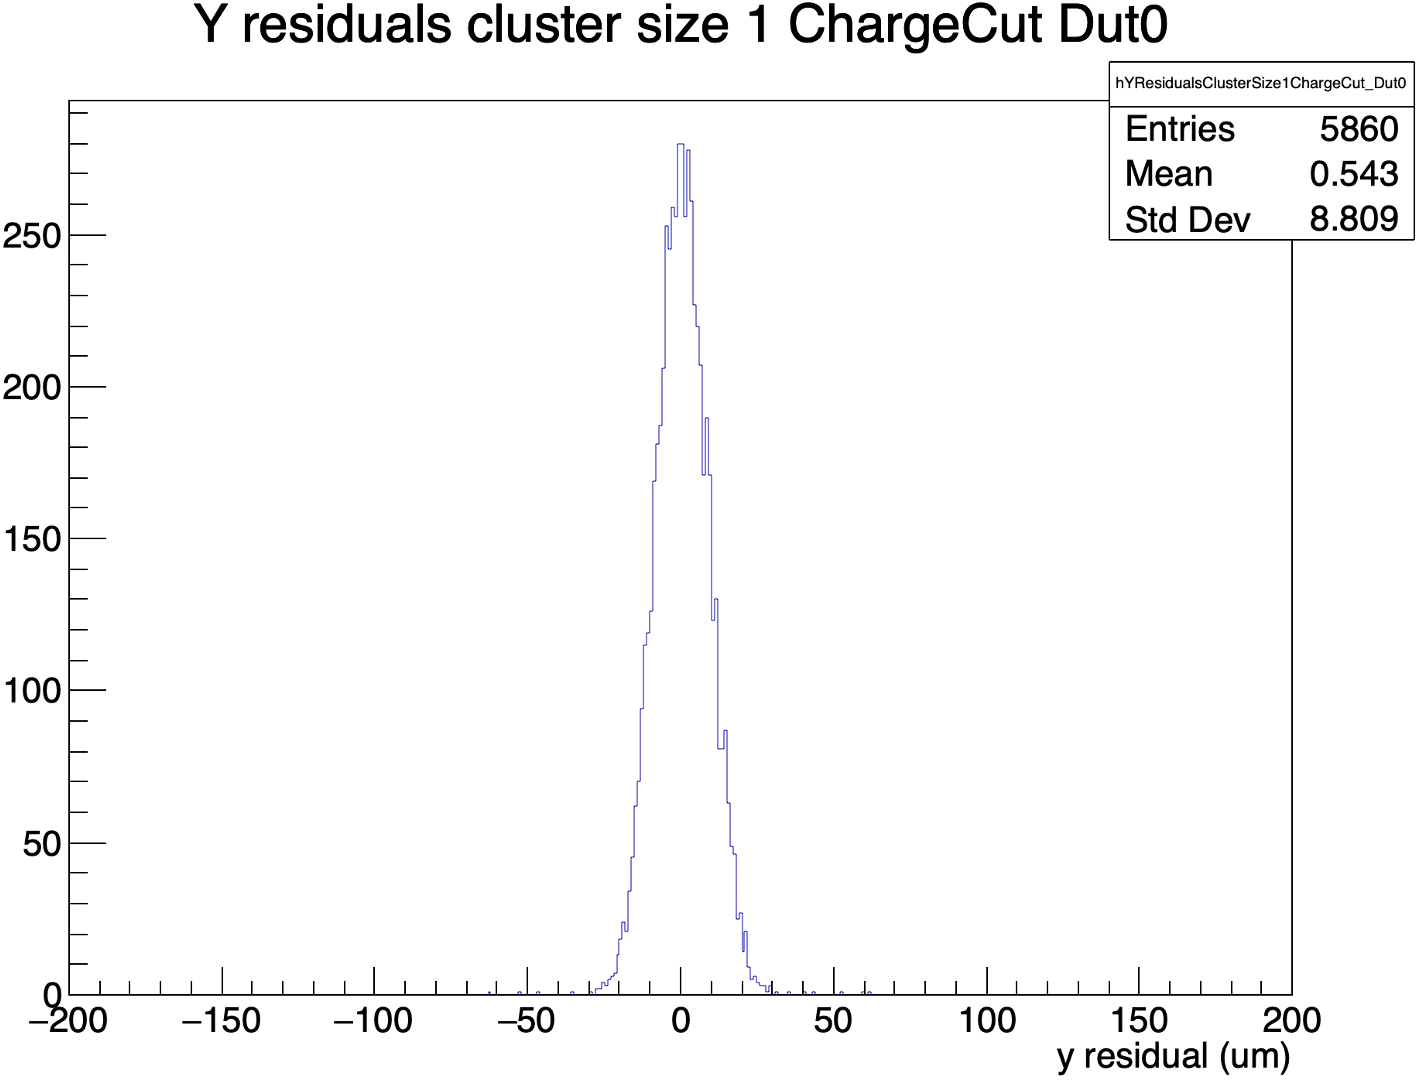
\includegraphics[width=\textwidth]{images/YRes_size1_4pixel.png}
        \caption{}
    \end{subfigure}
    \hfill
    \begin{subfigure}[b]{0.3\textwidth}
        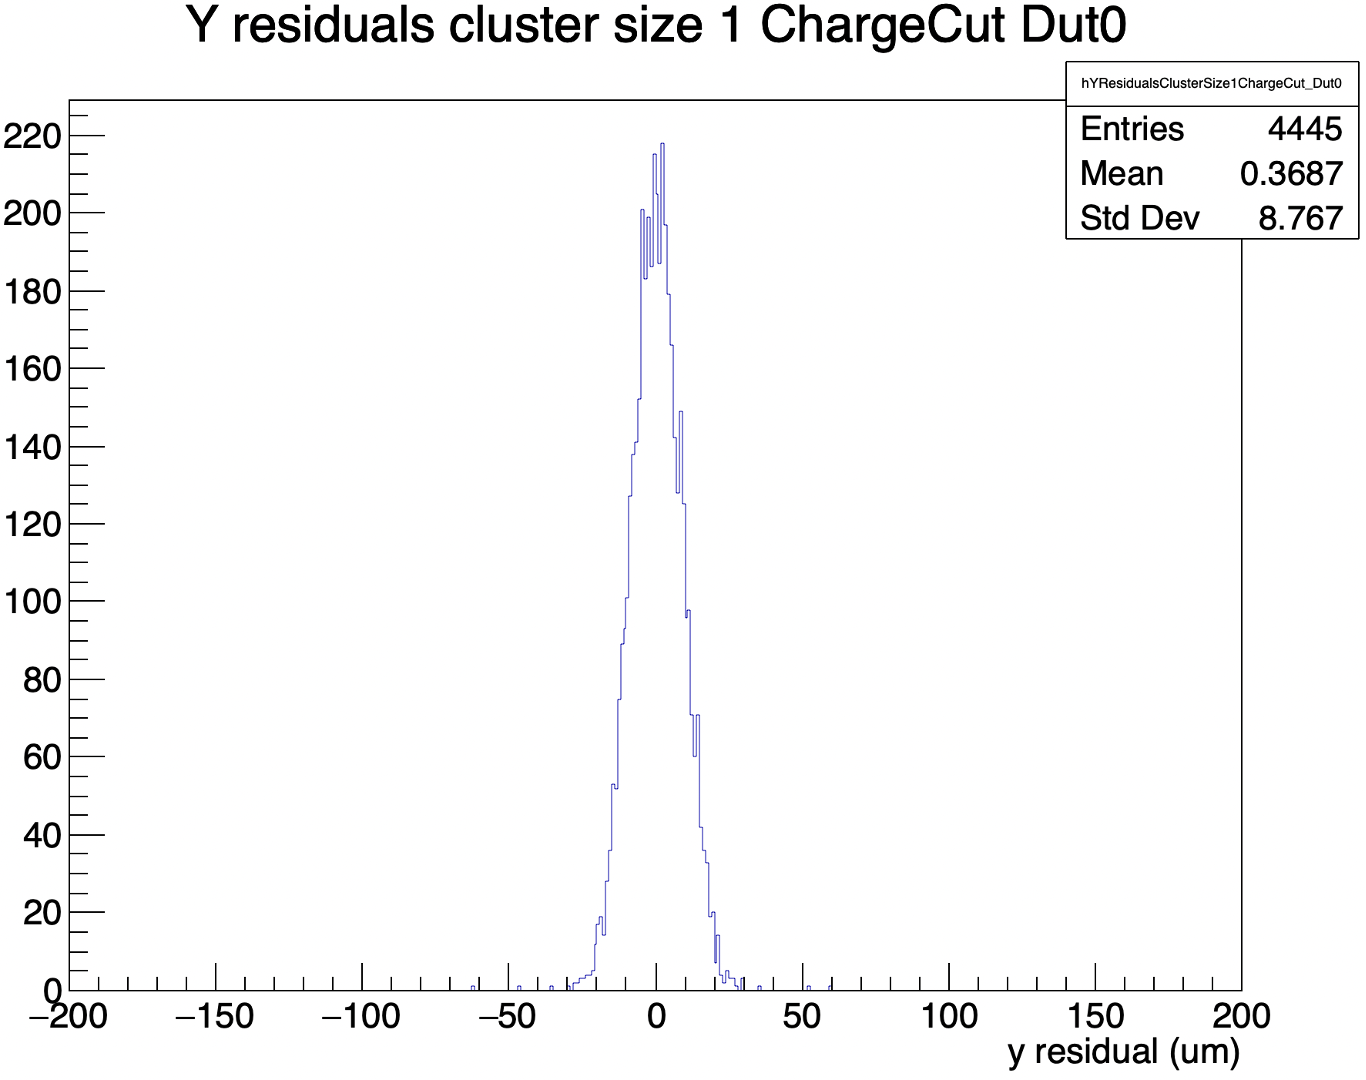
\includegraphics[width=\textwidth]{images/YRes_size1_4pixel_noBin0.png}
        \caption{}
    \end{subfigure}

    \caption{X residuals for cluster size 1 shown in (a--c): (a) using tracks that pass through at least 13 planes, (b) requiring tracks to pass through all 4 pixel planes, and (c) same as (b) but with Bin 0 (delta-ray) tracks excluded. Panels (d--f) show the corresponding Y residuals under the same conditions.}
    \label{fig:X_Y_Residual_size_1_planes}
\end{figure}

In addition, asymmetry plots for different charge Bins were studied, with the expectation that the delta-ray charge Bin~0 would be more asymmetric than the others, indicating higher crosstalk. The charge asymmetry is defined as
\[
\text{Asymmetry} = \frac{C_L - C_R}{C_L + C_R},
\]
where \( C_L \) and \( C_R \) are the charges collected by the cells to the left and right of the divide, respectively. The results for the right bump-bonded side are shown in Figure~\ref{fig:asymmetry_bins}. However, it is difficult to interpret the results for charge Bin~0 due to the relatively small number of entries compared to the other Bins. Furthermore, it was observed that data points near the asymmetry values of 1 and $-1$ mostly correspond to charge-shared clusters. Despite this, a clear interpretation is still challenging, as no quantitative measure of the asymmetry has been established so far. Therefore, further investigation is needed for better understanding of this behavior.

\begin{figure}[H]
    \centering
    \begin{subfigure}[t]{0.45\textwidth}
        \centering
        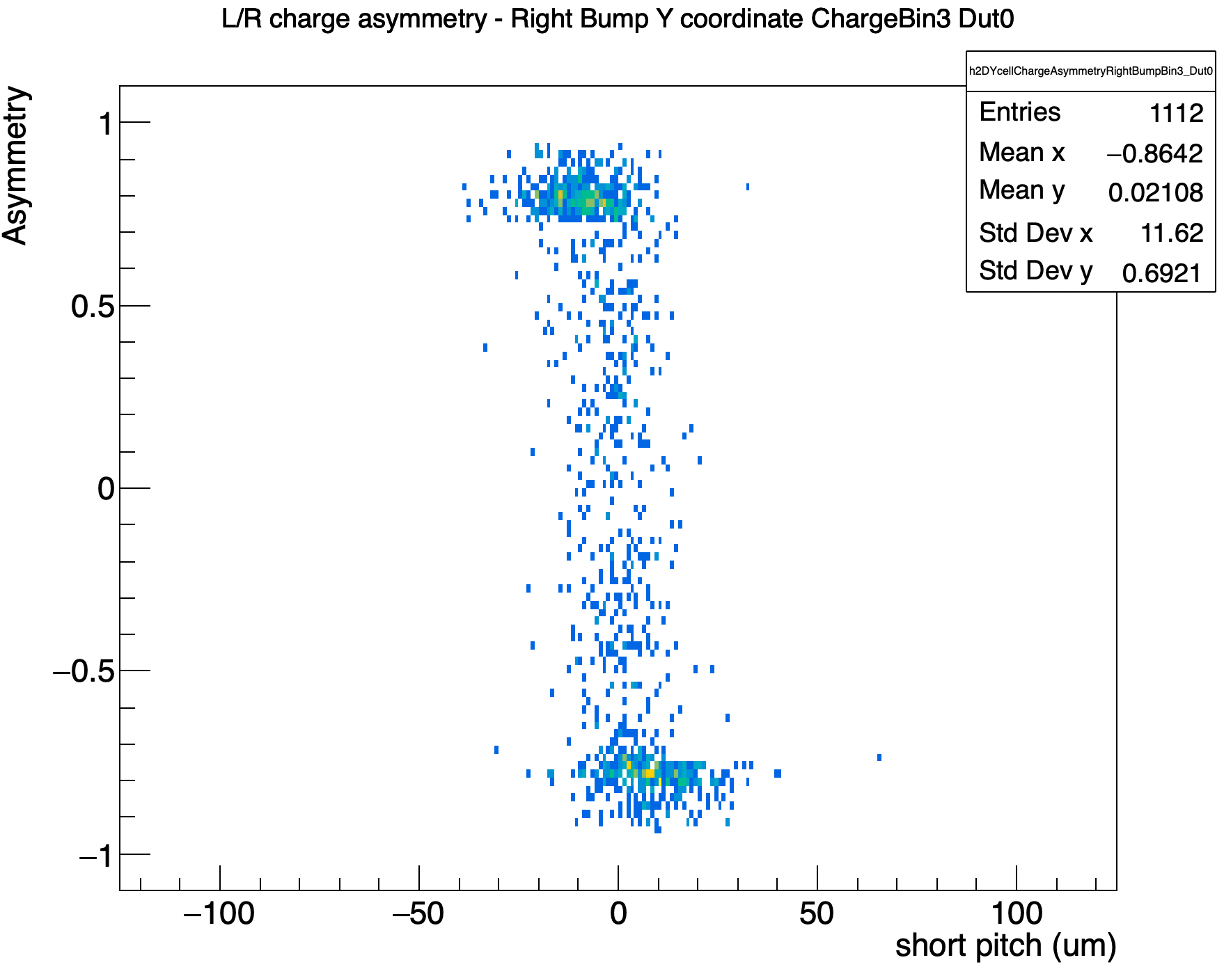
\includegraphics[width=\textwidth]{images/YAsymBin3.png}
        \caption{}
        \label{fig:dist_a}
    \end{subfigure}
    \hfill
    \begin{subfigure}[t]{0.45\textwidth}
        \centering
        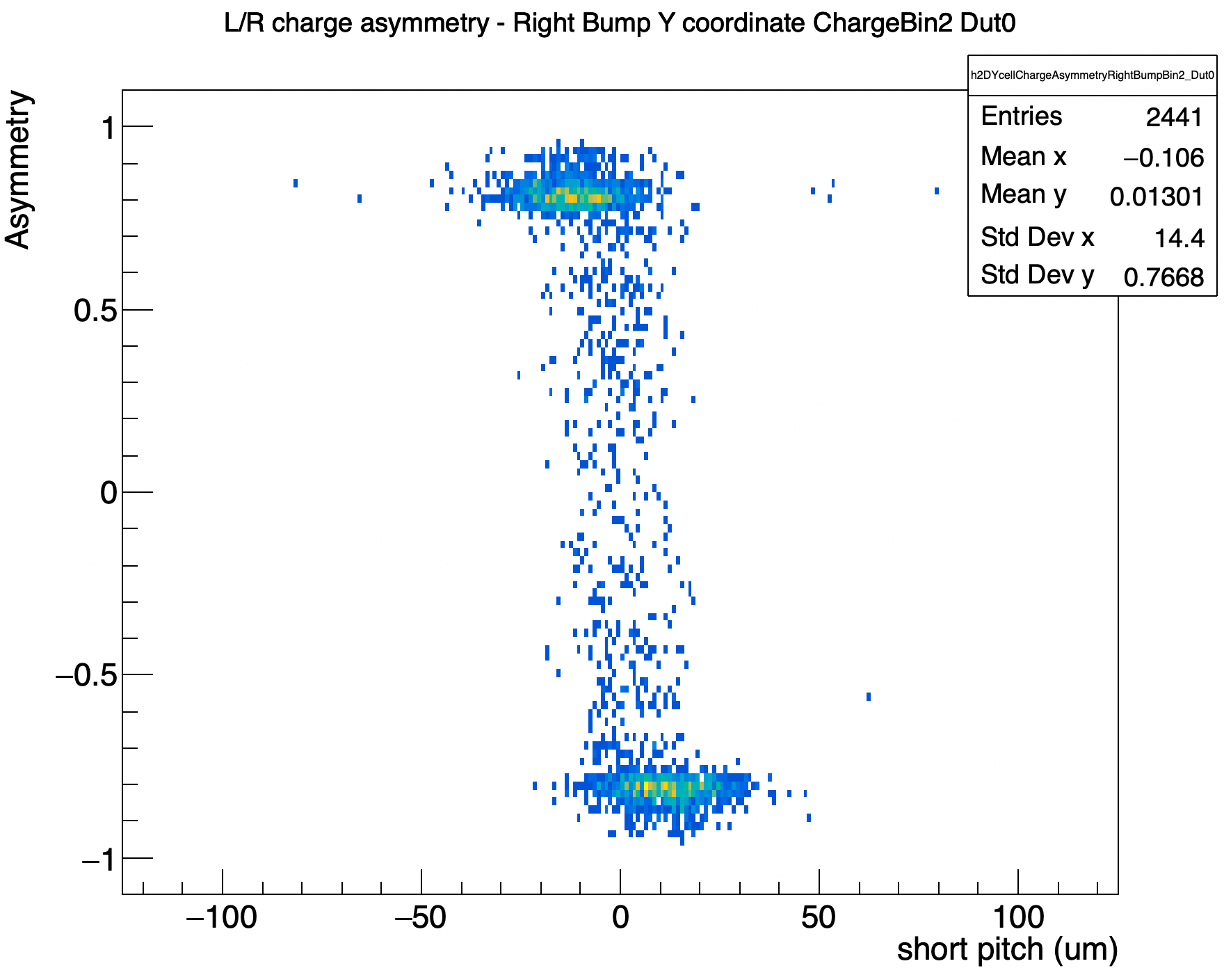
\includegraphics[width=\textwidth]{images/YAsymBin2.png}
        \caption{}
        \label{fig:dist_b}
    \end{subfigure}

    \vspace{0.5cm}

    \begin{subfigure}[t]{0.45\textwidth}
        \centering
        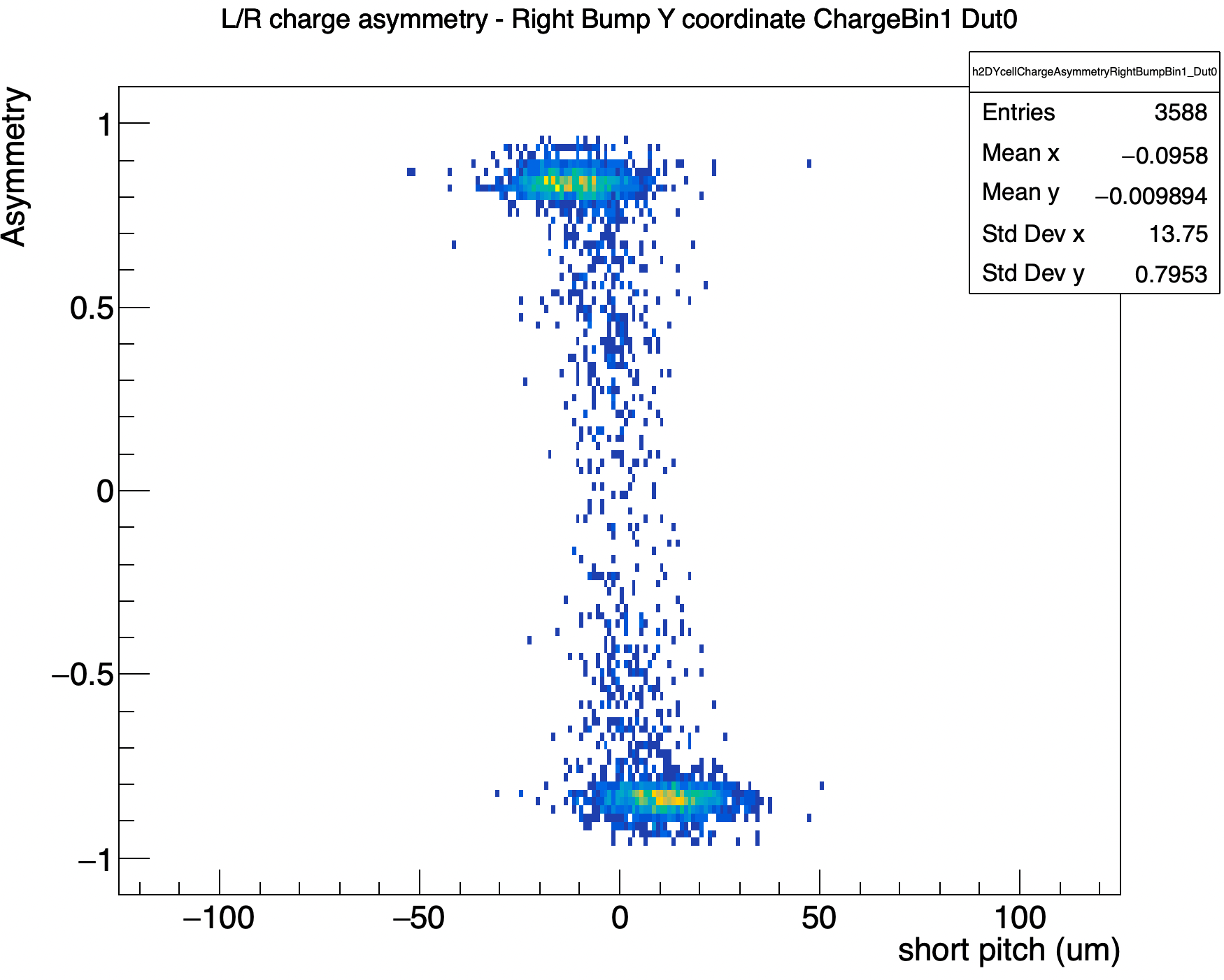
\includegraphics[width=\textwidth]{images/YAsymmetryRightBin1.png}
        \caption{}
        \label{fig:dist_c}
    \end{subfigure}
    \hfill
    \begin{subfigure}[t]{0.45\textwidth}
        \centering
        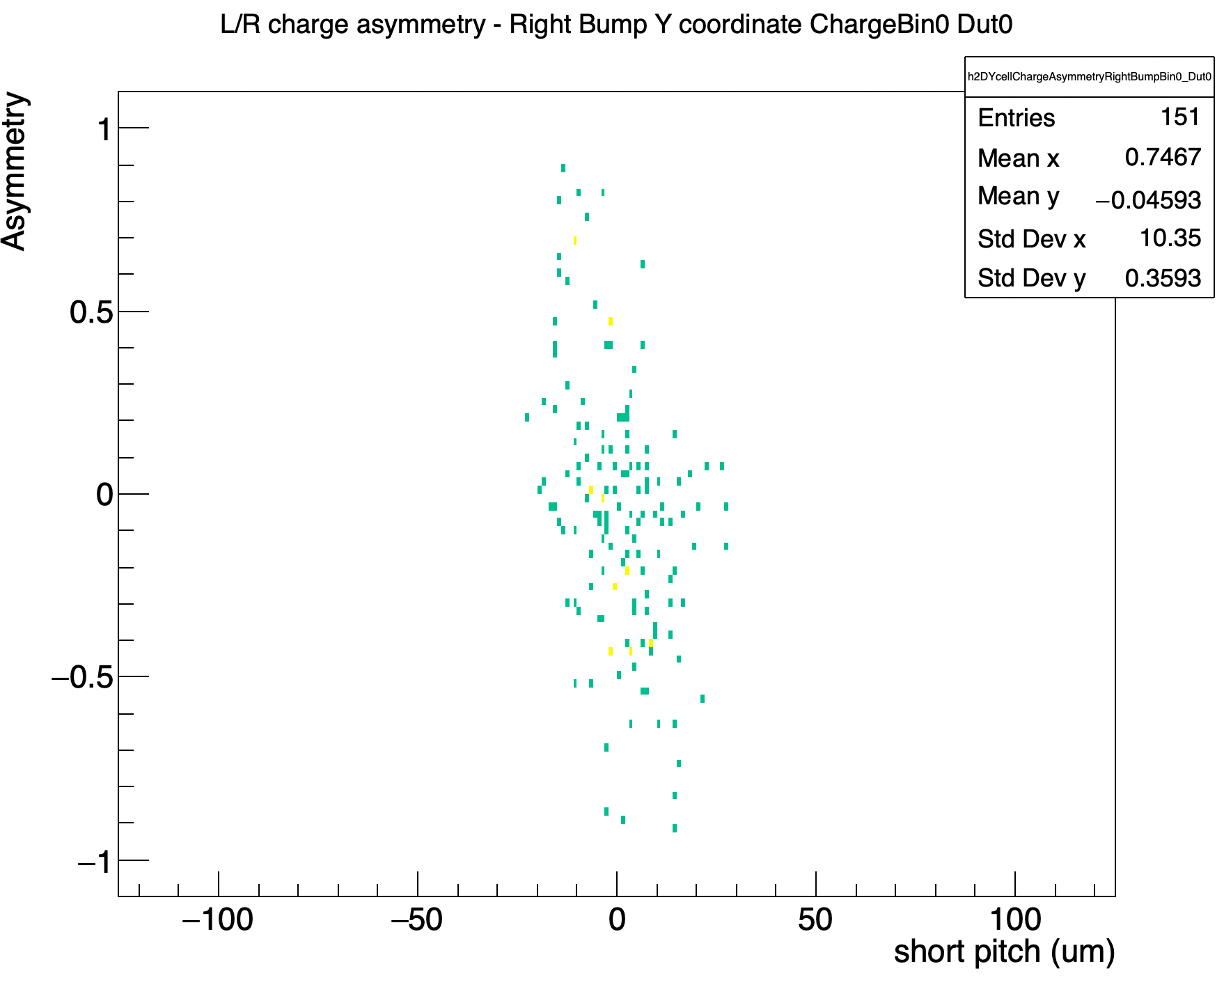
\includegraphics[width=\textwidth]{images/YAsymmetryRightBumpBin0.png}
        \caption{}
        \label{fig:dist_d}
    \end{subfigure}

    \caption{Asymmetry plot for all of the charge Bins.}
    \label{fig:asymmetry_bins}
\end{figure}

\subsection{NMF for 1D Data Quality Monitoring}

Typically, input data are represented by a particular ME (1D so far) for each LS of the RR, and after some minor filtering, the model is trained on it. Test or target data have the training data as a reference used for certification. After some prefiltering based on the basis matrix, the coefficient matrix for the test data may be found. However, in order to identify actual anomalies and prove the concept of the model, fake test data were produced such that the first LS corresponds to an actual LS from the training data. In particular, in this case, the charge distribution for Pixel Layer 1 was observed. The remaining LSs were generated by shifting the peak of the Landau-like distribution to the left, bin by bin. The total number of generated fake data LSs is 14 see Figure~\ref{fig:fake_data}.

\begin{figure}[H]
    \centering
    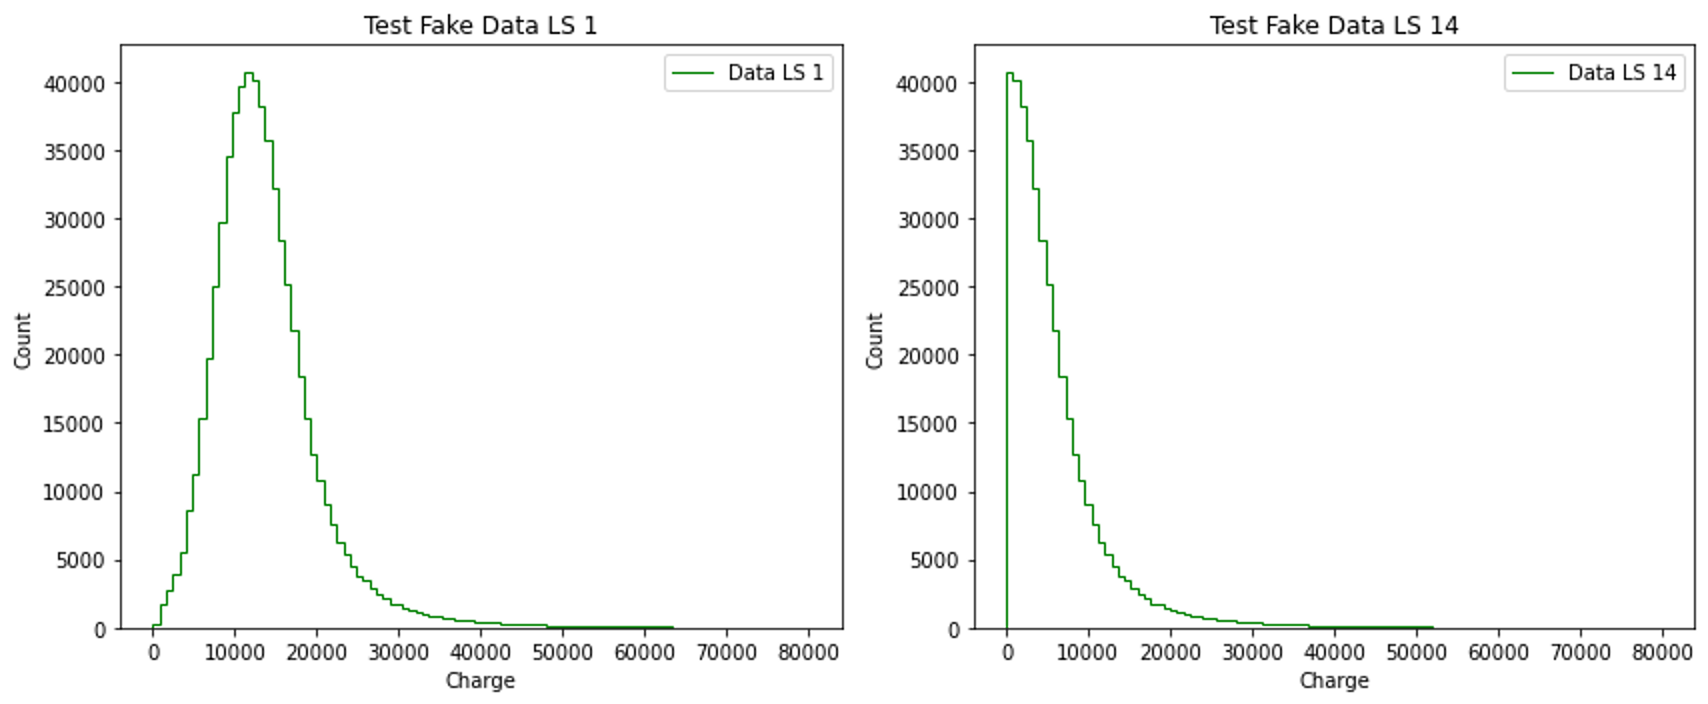
\includegraphics[width=0.9\textwidth]{images/fake_input.png}
    \caption{Fake data generated (first and last LSs) for the NMF model. The first LS corresponds to the actual data, while the remaining LSs are shifted by one bin to the left.}
    \label{fig:fake_data}
\end{figure}

The model was trained on one of the RRs. The optimal number of components for this case is 4. The basis components are shown in Figure~\ref{fig:components}. It is clearly noticeable that the first component is dominant and represents the main trend of the data (not normalized). The other components are shifted distributions. These components reconstruct the target fake data with different weights assigned to each of them.

\begin{figure}[H]
    \centering
    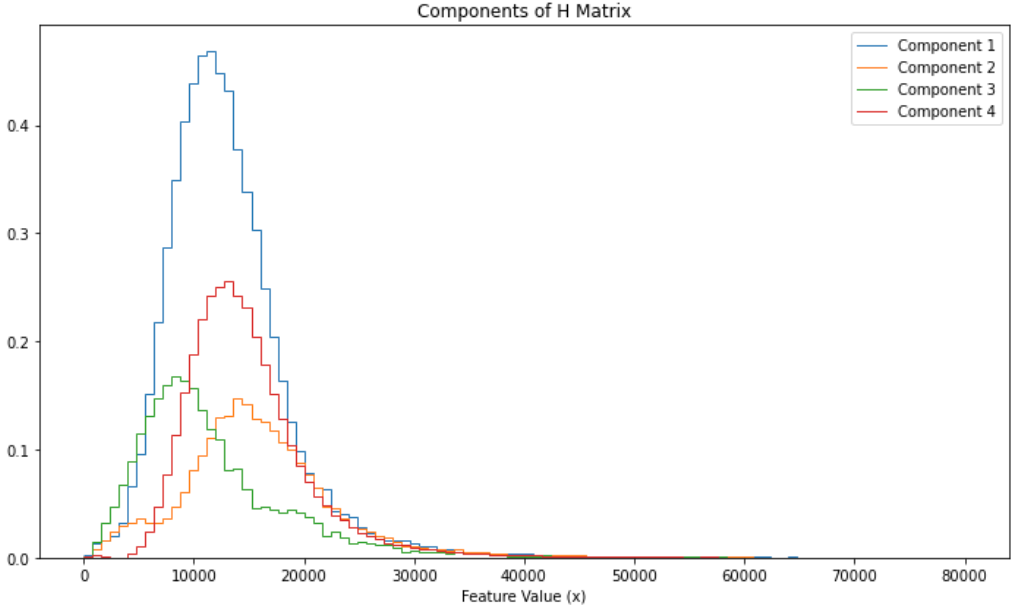
\includegraphics[width=0.8\textwidth]{images/Hcomponents.png}
    \caption{Basis components out of the \( H \) matrix.}
    \label{fig:components}
\end{figure}

\begin{figure}[H]
    \centering
    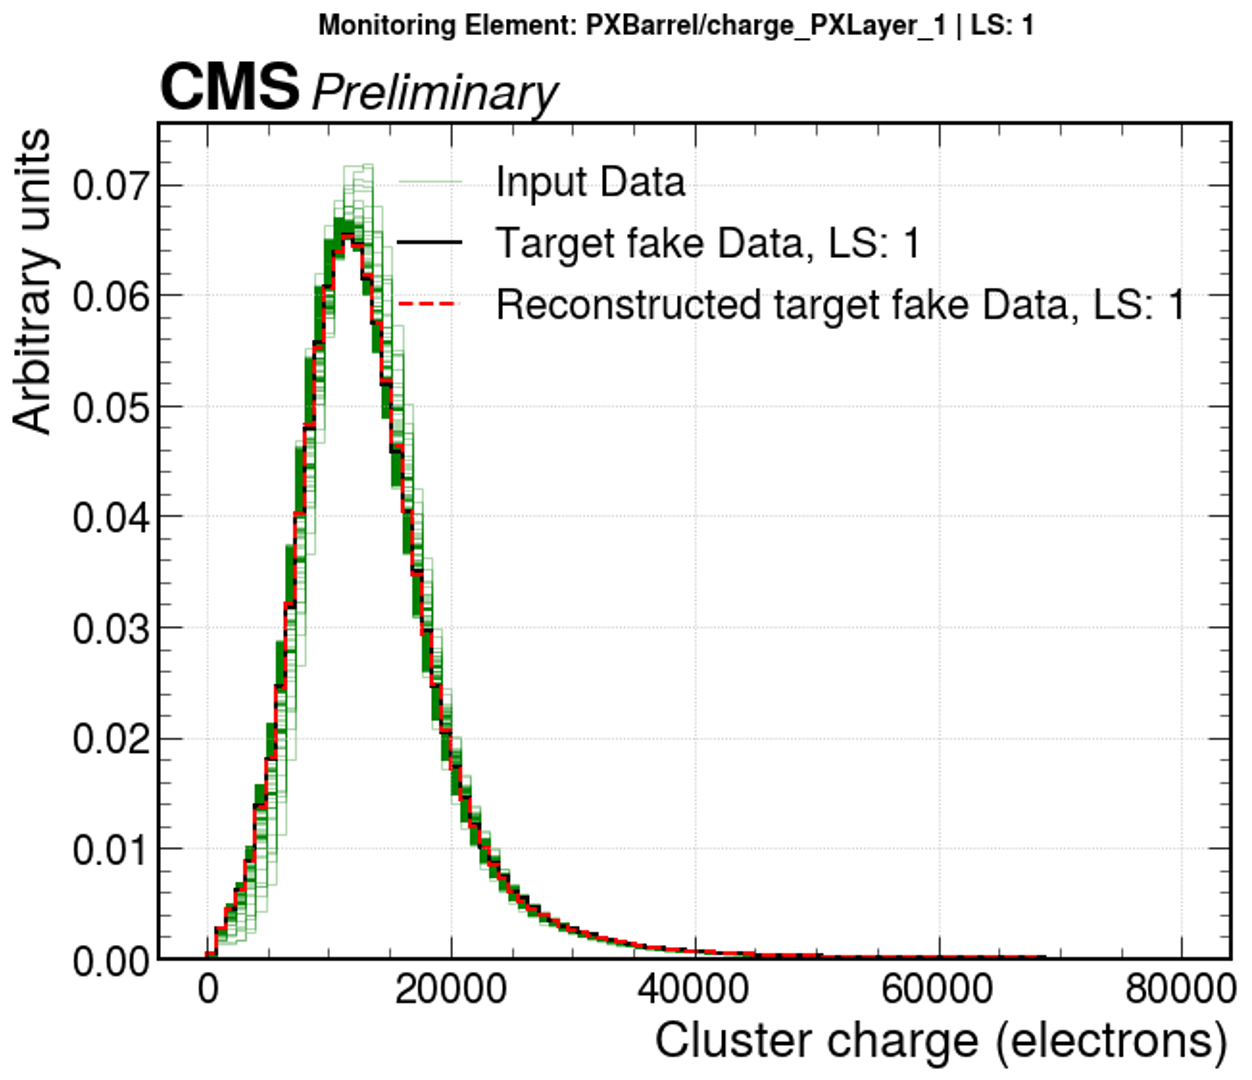
\includegraphics[width=0.48\textwidth]{images/fake_reco_ls1.png}
    \hfill
    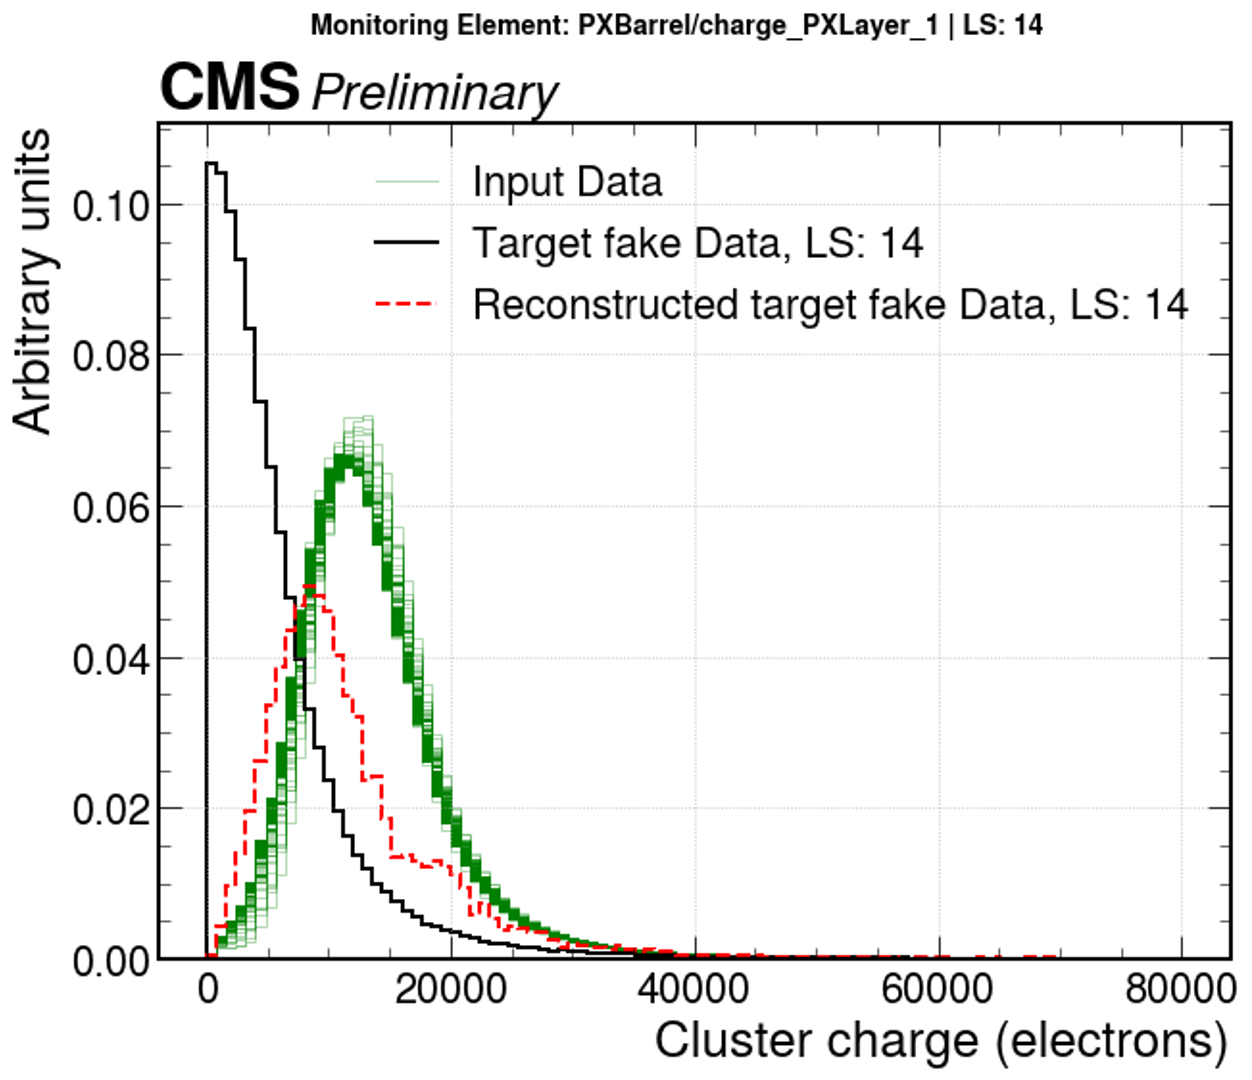
\includegraphics[width=0.48\textwidth]{images/fake_reco_ls14.png}
    \caption{Reconstruction of the 1st (left) and 14th (right) LSs from the fake dataset. The red lines show the model’s reconstruction of fake data, while the green lines represent the overlaid histograms from all training LSs, serving as a reference.}
    \label{fig:reconstruction}
\end{figure}

The reconstruction of these two LSs of the fake data is shown in Figure~\ref{fig:reconstruction}. The label "Input data" corresponds to the training data and is shown in the figures in green. These green histograms represent all of the training data LSs overlaid in order to compare the shifts of the training data with the target fake data. Since the first LS corresponds to actual, true data, its reconstruction looks good and is represented by a noticeable red histogram. Red reconstruction histogram for the first LS overlap with the green ones. However, for the last LS which has the maximum shift in the charge distribution, the reconstruction clearly fails. The red histogram again represents the reconstruction, with the same overlay of training data in green. Therefore, this LS is clearly anomalous. However, in order to apply the model to real data, it is necessary to define a metric to determine the anomaly threshold.

Metrics chosen for identifying anomaly:
\begin{itemize}
    \item Trends for component by the contribution of the area to the distribution see Figure~\ref{fig:trend_plots}
    \item Euclidean distance see Figure~\ref{fig:euc_distance}
    \item Mean squared error (MSE) see Figure~\ref{fig:MSE}
\end{itemize}

The trend plots show the contribution of each component in area to the reconstruction (Figure~\ref{fig:trend_plots}). The mean and standard deviation are shown in the labels for both the training and fake test data. If the contribution of any component in the test data falls outside the range of the training mean \( \pm\,2\sigma \), the corresponding LS is considered an outlier. In particular, the components for LS~3 clearly fall outside the expected range. Additionally, component~4 does not contribute to the reconstruction of the test data.

The Euclidean distance error was calculated for the training data by first determining the center of the training dataset in the latent space. This center represents the average position of all lumisections (LSs) across the defined components. The distance of each LS to this center is then computed. A cut is established as the mean \( \pm\,2\sigma \). Any LS from the test dataset whose distance exceeds this threshold is flagged as anomalous. This method successfully flags LSs starting from the 3rd one, which aligns well with the known shift applied to the fake data. Although the 2nd LS is also synthetic, the shift in its distribution is too small to be detected by this criterion.

\begin{figure}[H]
    \centering
    \begin{subfigure}[t]{1\textwidth}
        \centering
        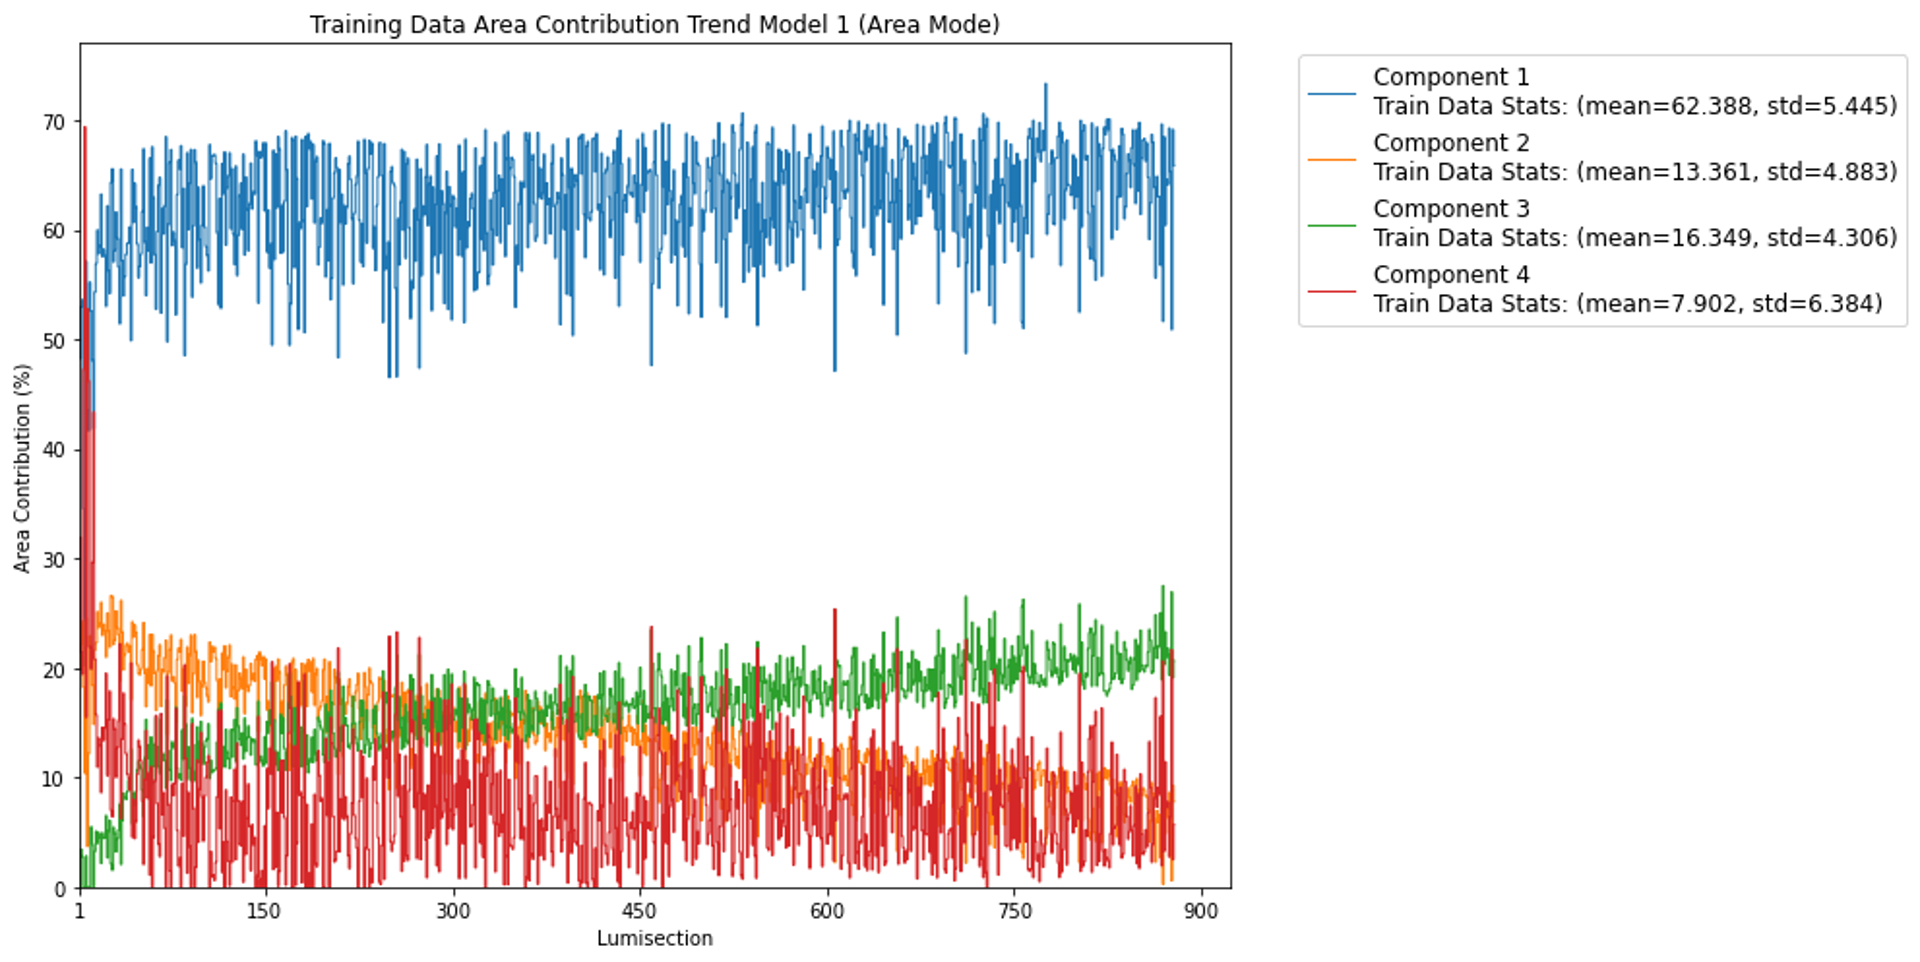
\includegraphics[width=\textwidth]{images/trend_train.png}
    \end{subfigure}
    \hfill
    \begin{subfigure}[t]{1\textwidth}
        \centering
        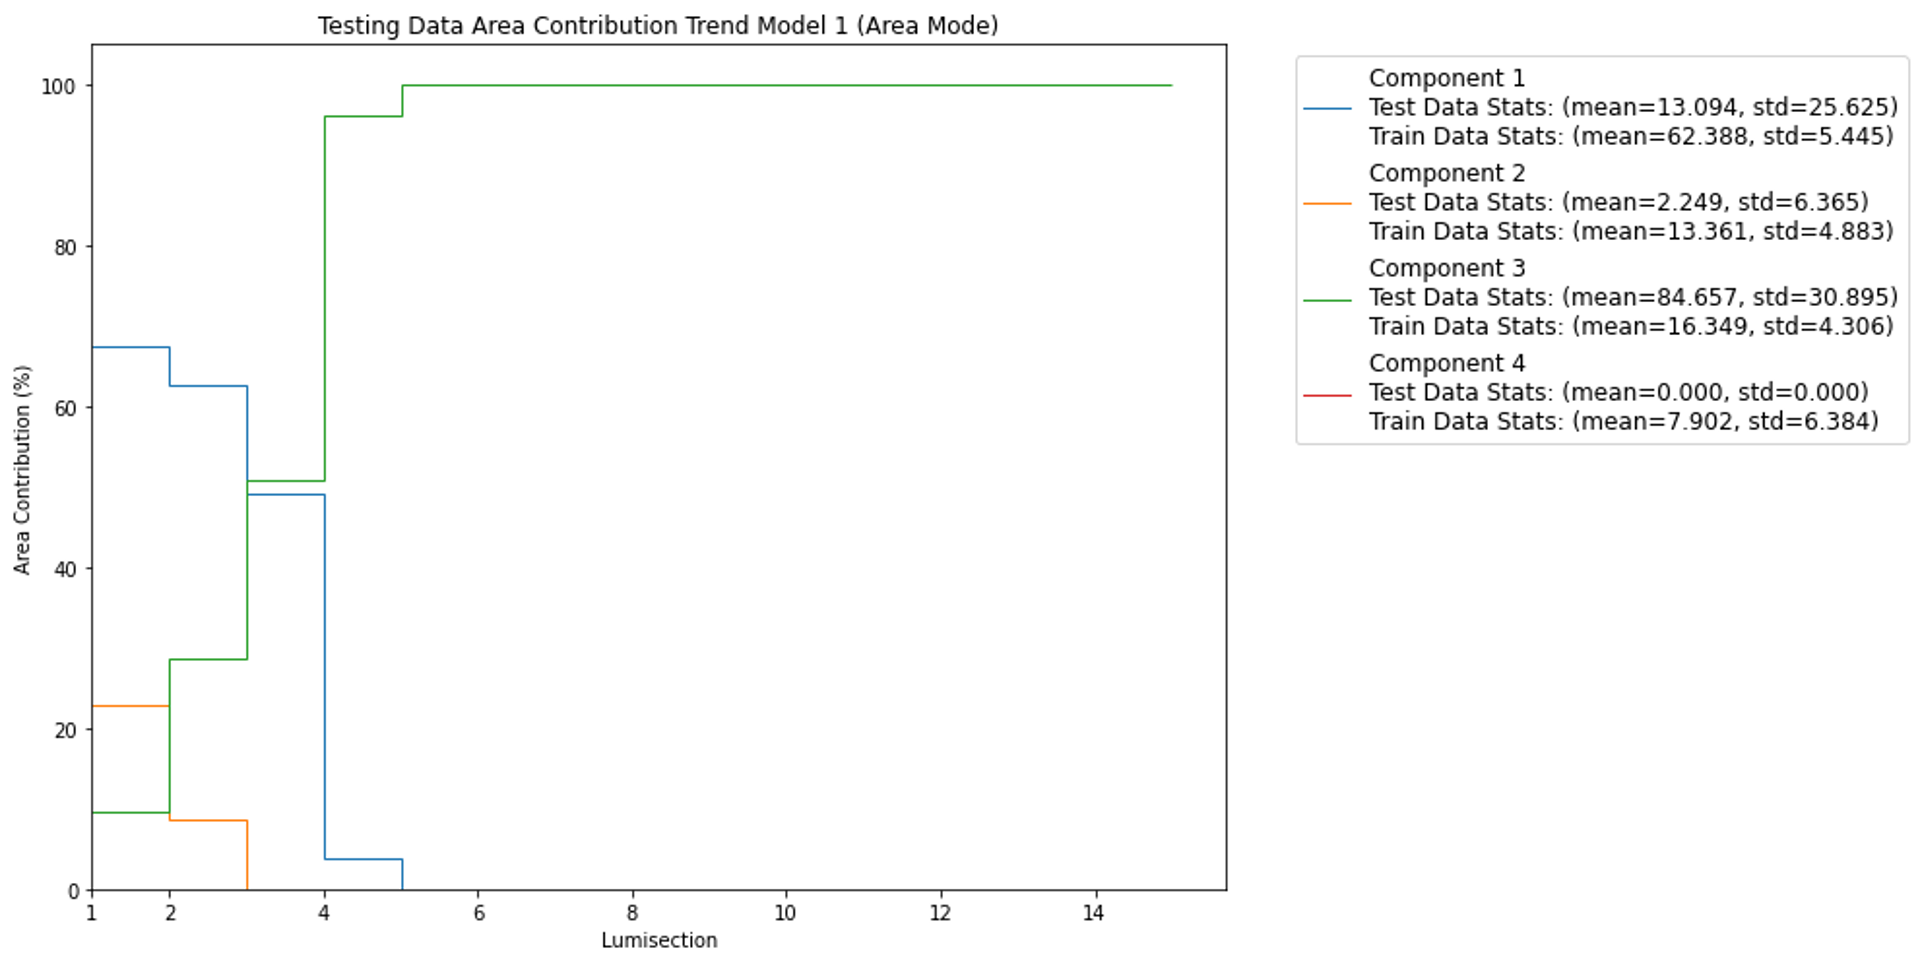
\includegraphics[width=\textwidth]{images/trend_fake.png}
    \end{subfigure}
    \caption{Trend plots showing the percentage area contribution of each component to the reconstruction. The top row displays trends from the training data, with the mean and standard deviation for each component indicated in the legend. The bottom row presents trends from the fake test data, where both training and test statistics (mean and standard deviation) are shown for comparison.}
    \label{fig:trend_plots}
\end{figure}

\begin{figure}[H]
    \centering
    \begin{subfigure}[t]{1\textwidth}
        \centering
        \includegraphics[width=\textwidth]{images/euclid_train.png}
    \end{subfigure}
    \hfill
    \begin{subfigure}[t]{1\textwidth}
        \centering
        \includegraphics[width=\textwidth]{images/euclid_test_fake.png}
    \end{subfigure}
    \caption{Euclidean distance error for the training data (top) and test data (bottom). A threshold, defined from the training data (indicated by the green horizontal line), is applied to the test data to identify anomalous behavior.}
    \label{fig:euc_distance}
\end{figure}

The MSE is calculated for the training data, with a threshold defined at 99\%. LSs from the training data that exceed this threshold are excluded from further consideration. When the same criterion is applied to the test data, LS~3 and subsequent LSs are flagged as anomalous, which aligns well with the results obtained using the previous metrics.

All of the applied metrics yield consistent and reasonable results. Although they may require further tuning to minimize false positives when applied to real data, the underlying concept is effective. The approach is extendable to other MEs, with the primary goal being to deploy the model on real collision data from the 2024 run. Each metric will assign an anomaly score to any LS identified as anomalous, providing a quantitative basis for further investigation.

\begin{figure}[H]
    \centering
    \begin{subfigure}[t]{1\textwidth}
        \centering
        \includegraphics[width=\textwidth]{images/MSE_train.png}
    \end{subfigure}
    \hfill
    \begin{subfigure}[t]{1\textwidth}
        \centering
        \includegraphics[width=\textwidth]{images/MSE_test.png}
    \end{subfigure}
    \caption{MSE error for the training data (top) and test data (bottom). A threshold, defined from the training data (indicated by the green horizontal line), is applied to the test data to identify anomalous behavior.}
    \label{fig:MSE}
\end{figure}

% 


\chapter{Results}

% \section{Section}
% \noindent \lipsum[1][1-3] %WRITE HERE

% \subsection{Subsection}
% \noindent \lipsum[1][3-5] %WRITE HERE

% \subsubsection{Subsubsection}
% \noindent \blindtext %WRITE HERE

% \subsection{Subsection}
% \noindent \lipsum[1][2-5] %WRITE HERE

%

% \chapter{Results}

% % \section{Section}
% % \noindent \lipsum[1][1-3] %WRITE HERE

% % \subsection{Subsection}
% % \noindent \lipsum[1][3-5] %WRITE HERE

% % \subsubsection{Subsubsection}
% % \noindent \blindtext %WRITE HERE

% % \subsection{Subsection}
% % \noindent \lipsum[1][2-5] %WRITE HERE

% % \subsubsection{Subsubsection}
% % \noindent \lipsum[1][1-5] %WRITE HERE

% % \section{Section}
% % \noindent \lipsum[1][5-8] %WRITE HERE

% % \subsection{Subsection}
% % \noindent \lipsum[1][9-15] %WRITE HERE





\chapter{Conclusions}

% \section{Section}
% \noindent \lipsum[1][1-5] %WRITE HERE


% \noindent \lipsum[1][1-5] %WRITE HERE


% \subsection{Subsection}
% \noindent \lipsum[1][1-5] %WRITE HERE


% \noindent \lipsum[1][1-5] %WRITE HERE

% \subsection{Subsection}
% \noindent \lipsum[1][1-5] %WRITE HERE


% \noindent \lipsum[1][1-5] %WRITE HERE

%\bibliographystyle{plain}
\bibliography{referencias}
\addcontentsline{toc}{chapter}{References}
\newpage


% %______________APPENDICES CONTENT______________________________
% % _____________APPENDIX A______________________________________
% \addcontentsline{exp}{chapter}{Appendix A: MATLAB Code} %Change title of Appendix A for List of Appendices
% %\example{MATLAB CODE}
% %\label{1st_ex}
% \chapter*{Appendix A: MATLAB Code} %Change title of Appendix A

% \noindent \lipsum[1][1-20] %WRITE HERE
% \noindent \lipsum[1][1-20] %WRITE HERE
% \noindent \lipsum[1][1-20] %WRITE HERE


% \newpage

% % _____________APPENDIX B______________________________________
% \addcontentsline{exp}{chapter}{Appendix B: Data} %Change title of Appendix B for List of Appendices
% \chapter*{Appendix B: Data} %Change title of Appendix B
% %\example{DATA}
% %\label{2nd_ex}
% \noindent \lipsum[1][1-3] %WRITE HERE

% \newpage

% % _____________APPENDIX C______________________________________
% \addcontentsline{exp}{chapter}{Appendix C: More Data} %Change title of Appendix C for List of Appendices
% \chapter*{Appendix C: More Data} %Change title of Appendix C
% %\example{DATA}
% %\label{2nd_ex}
% \noindent \lipsum[1][1-3] %WRITE HERE


% % _____________APPENDIX D______________________________________
% \addcontentsline{exp}{chapter}{Appendix D: More Data} %Change title of Appendix D for List of Appendices
% \chapter*{Appendix D: More Data} %Change title of Appendix C
% %\example{DATA}
% %\label{2nd_ex}
% \noindent \lipsum[1][1-3] %WRITE HERE

\end{document}
